% Baylor University Thesis LaTeX template
%- Template created by Jonathan Drake (2013)
% - Template updated by Kenneth Call, Kenichi Hatakeyama (2019)
% - Template updated by Chris Madrid, Caleb Smith (2020)

% Thesis class, based on report
\documentclass
[
	%short,	% omit front matter
	%draft, % draft heading, don't load graphics, etc.
]
{thesis}

% Optional additional packages
\usepackage{appendix}
\usepackage{etoolbox}
\usepackage{graphicx}
\usepackage{epstopdf}
\usepackage{amsmath}
\usepackage{chicago}
\usepackage{lipsum} % Because this comes with a demo
%\usepackage[hang, flushmargin, symbol]{footmisc}
\usepackage[hyperfootnotes=false, hidelinks=true]{hyperref}  % for workin links and bookmarks (alexsalo)
\usepackage[capitalise,nameinlink]{cleveref}  % used to format references to ranges of references.
\usepackage{bookmark}  % faster bookmarks manegment (alexsalo)
\usepackage{ifthen}
\usepackage[binary-units]{siunitx} %Easier use of scientific notation (Check also CMS defined units)
%\usepackage{topcapt} %This lets us put the table caption at the top using \topcaption
\usepackage{amssymb}
\usepackage{acronym} %This is used to create the List of acronyms
\usepackage[nobreak]{cite}
\usepackage{xspace}
\usepackage{xcolor}
\usepackage{slashed}
\usepackage{pdfpages}
\usepackage[textsize=footnotesize,textwidth=2.7cm]{todonotes}
\usepackage{footnotebackref}
\usepackage{adjustbox}
\usepackage{rotating}
\usepackage{tabu}

%%KC: Graduate school asks that references to chapters use words for the numbers. the fmtcount package translates number to words. This is really rather hacky. If the formated label is an integer according to xstring, then we set the hackyCounter to have that label's value, then print it using \Numberstring
\usepackage{fmtcount, xstring}

\newcount\hackyCounter
\newcounter{hackyCounter}

\creflabelformat{chapter}{#2\IfInteger{#1}{\setcounter{hackyCounter}{#1}\Numberstring{hackyCounter}}{#1}#3}

% using cleveref for appendices
% https://tex.stackexchange.com/questions/119513/cleveref-and-appendix-packages-appendix-referenced-as-section
\AtBeginEnvironment{appendices}{\crefalias{chapter}{appendix}}

%%special commands
%\setlength{\marginparwidth}{4cm}
\newcommand{\tinytodo}[2][]
{\todo[caption={#2}, #1]{\renewcommand{\baselinestretch}{0.8}\selectfont#2\par}}
\newcommand{\fxnote}[1]{\tinytodo{#1}}
\newcommand{\fixme}[1]{{\color{red}{FIXME: #1}}}
%\renewcommand{\footnote}[2][3]{\footnotemark[#1]\footnotetext[#1]{#2}}
\renewcommand{\chapterautorefname}{\mbox{Chapter}}
\renewcommand{\sectionautorefname}{\mbox{Section}}
\renewcommand{\subsectionautorefname}{\mbox{Section}}

%%Thesis parameters
\title{Electromagnetic and Hadronic Cluster Calibration for the CMS Particle Flow Algorithm Using Machine Learning Methods}    
\author{Noorah Asaad Ghazwani}
\holding{B.S.}
\seeking{M.S.}
\degree{Master of Science}
\project{A Thesis}
\date{00 2025}

%% Administration
\graduateDean{J.~Larry Lyon, Ph.D.}
\department{Department of Physics}
\departmentChair{Lorin Swint Matthews, Ph.D.}
\departmentChairTitle{Chairperson}

%% Supervisor (advisor / mentor)
\supervisor{Kenichi Hatakeyam, Ph.D.}
\supervisorRole{Advisor}

%% Readers (committee members)
\committee{Dissertation Committee}
\readerOne{Kenichi Hatakeyama Ph.D., Chairperson}
\readerTwo{Jay R. Dittmann, Ph.D.}
\readerThree{Andrew Brinkerhoff, Ph.D.}
\readerFour{not decided yet.}


%% CMS specific commands
%% \def\Fileversion$#1: #2 ${\gdef\fileversion{#2}}
%% \def\Filedate$#1: #2-#3-#4 #5 ${\gdef\filedate{#2/#3/#4}}
%% \Fileversion$Revision: 452536 $
%% \Filedate$Date: 2018-03-25 12:00:22 -0500 (Sun, 25 Mar 2018) $
%% %%%%%%%%%%%%%%%%%%%%%%%%%%%%%%%%%%%%%%%%%%%%%%%%%%%%%%%%%%%%%%%%%%%%
%% %
%% %  CMS Common definitions style file
%% %
%% %  N.B. use of \newcommand rather than \newcommand means
%% %       that a definition is ignored if already specified
%% %
%% %                                              L. Taylor 18 Feb 2005
%% %%%%%%%%%%%%%%%%%%%%%%%%%%%%%%%%%%%%%%%%%%%%%%%%%%%%%%%%%%%%%%%%%%%%
%% \NeedsTeXFormat{LaTeX2e}
%% \ProvidesPackage{ptdr-definitions}[\filedate\space CMS Additional Macro Definitions (\fileversion)]
\RequirePackage{xspace}
\RequirePackage{amsmath}

% Some shorthand
% turn off italics
\newcommand {\etal}{\mbox{et al.}\xspace} %et al. - no preceding comma
\newcommand {\ie}{\mbox{i.e.}\xspace}     %i.e.
\newcommand {\eg}{\mbox{e.g.}\xspace}     %e.g.
\newcommand {\etc}{\mbox{etc.}\xspace}     %etc.
\newcommand {\aka}{\mbox{aka.}\xspace}     %aka.
\newcommand {\vs}{\mbox{\sl vs.}\xspace}      %vs.
\newcommand {\mdash}{\ensuremath{\mathrm{-}}} % for use within formulas
\providecommand {\NA}{\ensuremath{\text{---}}}    % for Not applicable (or available). Needs to be renewcommanded for APS to \cdots

% some terms whose definition we may change
\newcommand {\Lone}{Level-1\xspace} % Level-1 or L1 ?
\newcommand {\Ltwo}{Level-2\xspace}
\newcommand {\Lthree}{Level-3\xspace}

% Some software programs (alphabetized)
\newcommand{\ACERMC} {\textsc{AcerMC}\xspace}
\newcommand{\ALPGEN} {{\textsc{alpgen}}\xspace}
\newcommand{\BLACKHAT} {{\textsc{BlackHat}}\xspace}
\newcommand{\CALCHEP} {{\textsc{CalcHEP}}\xspace}
\newcommand{\CHARYBDIS} {{\textsc{charybdis}}\xspace}
\newcommand{\CMKIN} {\textsc{cmkin}\xspace}
\newcommand{\CMSIM} {{\textsc{cmsim}}\xspace}
\newcommand{\CMSSW} {{\textsc{cmssw}}\xspace}
\newcommand{\COBRA} {{\textsc{cobra}}\xspace}
\newcommand{\COCOA} {{\textsc{cocoa}}\xspace}
\newcommand{\COMPHEP} {\textsc{CompHEP}\xspace}
\newcommand{\EVTGEN} {{\textsc{evtgen}}\xspace}
\newcommand{\FAMOS} {{\textsc{famos}}\xspace}
\newcommand{\FASTJET} {{\textsc{FastJet}}\xspace}
\newcommand{\FEWZ} {{\textsc{fewz}}\xspace}
\newcommand{\GARCON} {\textsc{garcon}\xspace}
\newcommand{\GARFIELD} {{\textsc{garfield}}\xspace}
\newcommand{\GEANE} {{\textsc{geane}}\xspace}
\newcommand{\GEANTfour} {{\textsc{Geant4}}\xspace}
\newcommand{\GEANTthree} {{\textsc{geant3}}\xspace}
\newcommand{\GEANT} {{\textsc{geant}}\xspace}
\newcommand{\HDECAY} {\textsc{hdecay}\xspace}
\newcommand{\HERWIG} {{\textsc{herwig}}\xspace}
\newcommand{\HERWIGpp} {{\textsc{herwig++}}\xspace}
\newcommand{\POWHEG} {{\textsc{powheg}}\xspace}
\newcommand{\HIGLU} {{\textsc{higlu}}\xspace}
\newcommand{\HIJING} {{\textsc{hijing}}\xspace}
\newcommand{\HYDJET} {{\textsc{hydjet}}\xspace}
\newcommand{\IGUANA} {\textsc{iguana}\xspace}
\newcommand{\ISAJET} {{\textsc{isajet}}\xspace}
\newcommand{\ISAPYTHIA} {{\textsc{isapythia}}\xspace}
\newcommand{\ISASUGRA} {{\textsc{isasugra}}\xspace}
\newcommand{\ISASUSY} {{\textsc{isasusy}}\xspace}
\newcommand{\ISAWIG} {{\textsc{isawig}}\xspace}
\newcommand{\MADGRAPH} {\textsc{MadGraph}\xspace}
\newcommand{\MCATNLO} {\textsc{mc@nlo}\xspace}
\newcommand{\MCFM} {\textsc{mcfm}\xspace}
\newcommand{\MILLEPEDE} {{\textsc{millepede}}\xspace}
\newcommand{\ORCA} {{\textsc{orca}}\xspace}
\newcommand{\OSCAR} {{\textsc{oscar}}\xspace}
\newcommand{\PHOTOS} {\textsc{photos}\xspace}
\newcommand{\PROSPINO} {\textsc{prospino}\xspace}
\newcommand{\PYTHIA} {{\textsc{pythia}}\xspace}
\newcommand{\SHERPA} {{\textsc{sherpa}}\xspace}
\newcommand{\TAUOLA} {\textsc{tauola}\xspace}
\newcommand{\TOPREX} {\textsc{TopReX}\xspace}
\newcommand{\XDAQ} {{\textsc{xdaq}}\xspace}
\newcommand{\MGvATNLO}{\MADGRAPH{}5\_a\MCATNLO}


%  Experiments
\newcommand {\DZERO}{D0\xspace}     %etc.


% Measurements and units...

\newcommand{\de}{\ensuremath{^\circ}}
\newcommand{\ten}[1]{\ensuremath{\times \text{10}^\text{#1}}}
\newcommand{\unit}[1]{\ensuremath{\text{\ #1}}\xspace}
\newcommand{\mum}{\ensuremath{\ \mu\text{m}}\xspace}
\newcommand{\micron}{\ensuremath{\ \mu\text{m}}\xspace}
\newcommand{\cm}{\ensuremath{\ \text{cm}}\xspace}
\newcommand{\mm}{\ensuremath{\ \text{mm}}\xspace}
\newcommand{\second}{\ensuremath{\ \text{s}}\xspace}
\newcommand{\mus}{\ensuremath{\ \mu\text{s}}\xspace}
\newcommand{\keV}{\ensuremath{\ \text{ke\hspace{-.08em}V}}\xspace}
\newcommand{\MeV}{\ensuremath{\ \text{Me\hspace{-.08em}V}}\xspace}
\newcommand{\MeVns}{\ensuremath{\text{Me\hspace{-.08em}V}}\xspace} % no leading thinspace
\newcommand{\GeV}{\ensuremath{\ \text{Ge\hspace{-.08em}V}}\xspace}
\newcommand{\GeVns}{\ensuremath{\text{Ge\hspace{-.08em}V}}\xspace} % no leading thinspace
\newcommand{\gev}{\GeV}
\newcommand{\TeV}{\ensuremath{\ \text{Te\hspace{-.08em}V}}\xspace}
\newcommand{\TeVns}{\ensuremath{\text{Te\hspace{-.08em}V}}\xspace} % no leading thinspace
\newcommand{\PeV}{\ensuremath{\ \text{Pe\hspace{-.08em}V}}\xspace}
\newcommand{\keVc}{\ensuremath{{\ \text{ke\hspace{-.08em}V\hspace{-0.16em}/\hspace{-0.08em}}c}}\xspace}
\newcommand{\MeVc}{\ensuremath{{\ \text{Me\hspace{-.08em}V\hspace{-0.16em}/\hspace{-0.08em}}c}}\xspace}
\newcommand{\GeVc}{\ensuremath{{\ \text{Ge\hspace{-.08em}V\hspace{-0.16em}/\hspace{-0.08em}}c}}\xspace}
\newcommand{\GeVcns}{\ensuremath{{\text{Ge\hspace{-.08em}V\hspace{-0.16em}/\hspace{-0.08em}}c}}\xspace} % no leading thinspace
\newcommand{\TeVc}{\ensuremath{{\ \text{Te\hspace{-.08em}V\hspace{-0.16em}/\hspace{-0.08em}}c}}\xspace}
\newcommand{\keVcc}{\ensuremath{{\ \text{ke\hspace{-.08em}V\hspace{-0.16em}/\hspace{-0.08em}}c^\text{2}}}\xspace}
\newcommand{\MeVcc}{\ensuremath{{\ \text{Me\hspace{-.08em}V\hspace{-0.16em}/\hspace{-0.08em}}c^\text{2}}}\xspace}
\newcommand{\GeVcc}{\ensuremath{{\ \text{Ge\hspace{-.08em}V\hspace{-0.16em}/\hspace{-0.08em}}c^\text{2}}}\xspace}
\newcommand{\GeVccns}{\ensuremath{{\text{Ge\hspace{-.08em}V\hspace{-0.16em}/\hspace{-0.08em}}c^\text{2}}}\xspace} % no leading thinspace
\newcommand{\TeVcc}{\ensuremath{{\ \text{Te\hspace{-.08em}V\hspace{-0.16em}/\hspace{-0.08em}}c^\text{2}}}\xspace}

\newcommand{\mb}{\ensuremath{\ \text{mb}}\xspace}
\newcommand{\mub}{\ensuremath{\ \mu\text{b}}\xspace}
\newcommand{\nbarn}{\ensuremath{\ \text{nb}}\xspace}
\newcommand{\pb}{\ensuremath{\ \text{pb}}\xspace}
\newcommand{\fb}{\ensuremath{\ \text{fb}}\xspace}
\newcommand{\mbinv}{\ensuremath{\ \text{mb}^{-1}}\xspace}
\newcommand{\mubinv}{\ensuremath{\ \mu\text{b}^{-1}}\xspace}
\newcommand{\nbinv}{\ensuremath{\ \text{nb}^{-1}}\xspace}
\newcommand{\pbinv}{\ensuremath{\ \text{pb}^{-1}}\xspace}
\newcommand{\fbinv}{\ensuremath{\ \text{fb}^{-1}}\xspace}
\newcommand{\percms}{\ensuremath{\ \text{cm}^\text{$-$2}\ \text{s}^\text{$-$1}}\xspace}
\newcommand{\lumi}{\ensuremath{\mathcal{L}}\xspace}
\newcommand{\Lumi}{\lumi}
\newcommand{\rate}{\ensuremath{\mathcal{R}}\xspace}
\newcommand{\Rate}{\rate}

% Need a convention here:
\newcommand{\LvLow}  {\ensuremath{\mathcal{L}=\text{10}^\text{32}\,\text{cm}^\text{$-$2}\,\text{s}^\text{$-$1}}\xspace}
\newcommand{\LLow}   {\ensuremath{\mathcal{L}=\text{10}^\text{33}\,\text{cm}^\text{$-$2}\,\text{s}^\text{$-$1}}\xspace}
\newcommand{\lowlumi}{\ensuremath{\mathcal{L}=\text{2}\times \text{10}^\text{33}\,\text{cm}^\text{$-$2}\,\text{s}^\text{$-$1}}\xspace}
\newcommand{\LMed}   {\ensuremath{\mathcal{L}=\text{2}\times \text{10}^\text{33}\,\text{cm}^\text{$-$2}\,\text{s}^\text{$-$1}}\xspace}
\newcommand{\LHigh}  {\ensuremath{\mathcal{L}=\text{10}^\text{34}\,\text{cm}^\text{$-$2}\,\text{s}^\text{$-$1}}\xspace}
\newcommand{\hilumi} {\ensuremath{\mathcal{L}=\text{10}^\text{34}\,\text{cm}^\text{$-$2}\,\text{s}^\text{$-$1}}\xspace}

% Physics symbols ...
\newcommand{\PT}{\ensuremath{p_{\mathrm{T}}}\xspace}
\newcommand{\pt}{\PT}
\newcommand{\pT}{\PT}
\newcommand{\ET}{\ensuremath{E_{\mathrm{T}}}\xspace}
\newcommand{\HT}{\ensuremath{H_{\mathrm{T}}}\xspace}
\newcommand{\et}{\ensuremath{E_{\mathrm{T}}}\xspace}
\newcommand{\Em}{\ensuremath{E\hspace{-0.6em}/}\xspace}
\newcommand{\Pm}{\ensuremath{p\hspace{-0.5em}/}\xspace}
\newcommand{\PTm}{\ensuremath{{p}_\mathrm{T}\hspace{-1.02em}/\kern 0.5em}\xspace}
\newcommand{\PTslash}{\PTm}
\newcommand{\ETm}{\ensuremath{E_{\mathrm{T}}^{\text{miss}}}\xspace}
\newcommand{\MET}{\ensuremath{p^{\rm miss}_{\rm T}}\xspace}
\newcommand{\METv}{\ensuremath{\vec{p}^{\rm miss}_{\rm T}}\xspace}
\newcommand{\ETmiss}{\ETm}
\newcommand{\ptmiss}{\ensuremath{\pt^\text{miss}}\xspace}
\newcommand{\ETslash}{\ensuremath{E_{\mathrm{T}}\hspace{-1.1em}/\kern0.45em}\xspace}
\newcommand{\VEtmiss}{\ensuremath{{\vec E}_{\mathrm{T}}^{\text{miss}}}\xspace}
\newcommand{\ptvec}{\ensuremath{{\vec p}_{\mathrm{T}}}\xspace}
\newcommand{\ptvecmiss}{\ensuremath{{\vec p}_{\mathrm{T}}^{\kern1pt\text{miss}}}\xspace}
\newcommand{\tauh}{\ensuremath{\PGt_\mathrm{h}}\xspace}
\newcommand{\sqrtsNN}{\ensuremath{\sqrt{\smash[b]{s_{_{\mathrm{NN}}}}}}\xspace}
\newcommand{\mht}{\ensuremath{H_{\mathrm{T}}^{\text{miss}}}\xspace}
\newcommand{\htvecmiss}{\ensuremath{\vec{H}_{\text{T}}^{\text{miss}}}\xspace}
\newcommand{\dphi}{\ensuremath{\Delta\phi}\xspace}
\newcommand{\MTTwo}{\ensuremath{m_{\text{T2}}}\xspace}
\newcommand{\mt}{\ensuremath{m_{\mathrm{T}}}\xspace}
\newcommand{\mT}{\mt}
\newcommand{\Mt}{\mt}
\newcommand{\MT}{\mt}
\newcommand{\mtb}{\ensuremath{\mt^\mathrm{\PQb}}\xspace}
\newcommand{\MTb}{\mtb}
\newcommand{\mTb}{\mtb}
\newcommand{\ptb}{\ensuremath{\pt^{\mathrm{\PQb}}}\xspace}
\newcommand{\ptbonetwo}{\ensuremath{\pt^{\mathrm{\PQb}_{12}}}}
\newcommand{\ptISR}{\ensuremath{\pt^{\text{ISR}}}\xspace}

\newcommand{\metsig}{\ensuremath{\ptmiss/\sqrt{H_\mathrm{T}}}\xspace}
\newcommand{\sipthreed}{{\tt SIP3D}\xspace}

% aliases to existing commands
\newcommand{\ptisr}{\ptISR}
\newcommand{\Ht}{\HT}
\newcommand{\met}{\MET}
\newcommand{\metv}{\METv}
\newcommand{\vMet}{\METv}
\newcommand{\vmet}{\METv}

% roman face derivative
\newcommand{\dd}[2]{\ensuremath{\frac{\cmsSymbolFace{d} #1}{\cmsSymbolFace{d} #2}}}
\newcommand{\ddinline}[2]{\ensuremath{\cmsSymbolFace{d} #1/\cmsSymbolFace{d} #2}}
\newcommand{\rd}{\ensuremath{\cmsSymbolFace{d}}}
\newcommand{\re}{\ensuremath{\cmsSymbolFace{e}}}
% absolute value
\newcommand{\abs}[1]{\ensuremath{\lvert #1 \rvert}}
% misc
\newcommand{\CL}{\ensuremath{\text{CL}}\xspace}
\newcommand{\CLs}{\ensuremath{\text{CL}_\text{s}}\xspace}
\newcommand{\CLsb}{\ensuremath{\text{CL}_\text{s+b}}\xspace}


%%%KH \ifthenelse{\boolean{cms@italic}}{\newcommand{\cmsSymbolFace}[1]{#1}}{\newcommand{\cmsSymbolFace}[1]{\mathrm{#1}}}
\newcommand{\cmsSymbolFace}[1]{\mathrm{#1}}

% Particle names which track the italic/non-italic face convention
\newcommand{\zp}{\ensuremath{{\cmsSymbolFace{Z}^\prime}}\xspace} % plain Z'
\newcommand{\JPsi}{\ensuremath{{\cmsSymbolFace{J}\hspace{-.08em}/\hspace{-.14em}\psi}}\xspace} % J/Psi (no mass)
\newcommand{\Z}{\ensuremath{\cmsSymbolFace{Z}}\xspace} % plain Z (no superscript 0)
\newcommand{\ttbar}{\ensuremath{{\cmsSymbolFace{t}\overline{\cmsSymbolFace{t}}}}\xspace} % t-tbar

% Extensions for missing names in PENNAMES % note no xspace, to match syntax in PENNAMES
\newcommand{\cPgn}{\ensuremath{\nu}} % generic neutrino
\providecommand{\Pgn}{\ensuremath{\nu}} % generic neutrino
\newcommand{\cPagn}{\ensuremath{\overline{\nu}}} % generic neutrino
\providecommand{\Pagn}{\ensuremath{\overline{\nu}}} % generic neutrino
\newcommand{\cPgg}{\ensuremath{\gamma}} % gamma
\newcommand{\cPJgy}{\ensuremath{\cmsSymbolFace{J}\hspace{-.08em}/\hspace{-.14em}\psi}} % J/Psi (no mass)
\newcommand{\cPW}{\ensuremath{\cmsSymbolFace{W}}} % W, no xspace
\newcommand{\cPZ}{\ensuremath{\cmsSymbolFace{Z}}} % plain Z (no superscript 0), no xspace
\newcommand{\cPZpr}{\ensuremath{\cmsSymbolFace{Z}'}} % plain Z'
\newcommand{\cPqt}{\ensuremath{\cmsSymbolFace{t}}} % t for t quark
\newcommand{\cPqb}{\ensuremath{\cmsSymbolFace{b}}} % b for b quark
\newcommand{\cPqc}{\ensuremath{\cmsSymbolFace{c}}} % c for c quark
\newcommand{\cPqs}{\ensuremath{\cmsSymbolFace{s}}} % s for s quark
\newcommand{\cPqu}{\ensuremath{\cmsSymbolFace{u}}} % u for u quark
\newcommand{\cPqd}{\ensuremath{\cmsSymbolFace{d}}} % d for d quark
\newcommand{\cPq}{\ensuremath{\cmsSymbolFace{q}}} % generic quark
\newcommand{\cPg}{\ensuremath{\cmsSymbolFace{g}}} % generic gluon
\newcommand{\cPG}{\ensuremath{\cmsSymbolFace{G}}} % Graviton
\newcommand{\cPaqt}{\ensuremath{\overline{\cmsSymbolFace{t}}}} % t for t anti-quark
\newcommand{\cPaqb}{\ensuremath{\overline{\cmsSymbolFace{b}}}} % b for b anti-quark
\newcommand{\cPaqc}{\ensuremath{\overline{\cmsSymbolFace{c}}}} % c for c anti-quark
\newcommand{\cPaqs}{\ensuremath{\overline{\cmsSymbolFace{s}}}} % s for s anti-quark
\newcommand{\cPaqu}{\ensuremath{\overline{\cmsSymbolFace{u}}}} % u for u anti-quark
\newcommand{\cPaqd}{\ensuremath{\overline{\cmsSymbolFace{d}}}} % d for d anti-quark
\newcommand{\cPaq}{\ensuremath{\overline{\cmsSymbolFace{q}}}} % generic anti-quark
\newcommand{\cPKstz}{\ensuremath{\cmsSymbolFace{K}^{\ast0}}\xspace} %note has xspace
% future symbols from heppennames2
\providecommand{\PGp}{\ensuremath{\pi}\xspace} % pi
\providecommand{\PGpp}{\ensuremath{\pi^+}\xspace} % pi
\providecommand{\PGpm}{\ensuremath{\pi^-}\xspace} % pi
\providecommand{\PGpz}{\ensuremath{\pi^0}\xspace} % pi
\providecommand{\PGr}{\ensuremath{\rho}\xspace} % pi
\providecommand{\PDast}{\ensuremath{\cmsSymbolFace{D}^\ast}\xspace} % D star
\providecommand{\PH}{\ensuremath{\cmsSymbolFace{H}}\xspace} % plain Higgs
\providecommand{\Ph}{\ensuremath{\cmsSymbolFace{h}}\xspace} % SUSY Higgs
\providecommand{\Pa}{\ensuremath{\cmsSymbolFace{a}}\xspace}
\providecommand{\PSA}{\ensuremath{\cmsSymbolFace{A}}\xspace} %pseudoscalar A Higgs
\providecommand{\PJGy}{\ensuremath{\cmsSymbolFace{J}\hspace{-.08em}/\hspace{-.14em}\psi}\xspace} % J/Psi (no mass)
\providecommand{\PBzs}{\ensuremath{\cmsSymbolFace{B}^0_\cmsSymbolFace{s}}\xspace} % B^0_s
\providecommand{\Pg}{\ensuremath{\cmsSymbolFace{g}}\xspace} % generic gluon
\providecommand{\PSg}{\ensuremath{\widetilde{\cmsSymbolFace{g}}}\xspace} % gluino
\providecommand{\PSQ}{\ensuremath{\widetilde{\cmsSymbolFace{q}}}\xspace} % squark
\providecommand{\PSGm}{\ensuremath{\widetilde{\mu}}\xspace} % smuon
\providecommand{\PSe}{\ensuremath{\widetilde{\cmsSymbolFace{e}}}\xspace} % selectron
\providecommand{\PASQ}{\ensuremath{\overline{\widetilde{\cmsSymbolFace{q}}}}\xspace} % anti quark
\providecommand{\PXXA}{\ensuremath{\cmsSymbolFace{A}}\xspace} % axion
\providecommand{\PXXG}{\ensuremath{\cmsSymbolFace{G}}\xspace} % graviton
\providecommand{\PXXSG}{\ensuremath{\widetilde{\PXXG}}\xspace} % gravitino
\providecommand{\PSGcp}{\ensuremath{\widetilde{\chi}^+}\xspace} % lightest positive chargino
\providecommand{\PSGcm}{\ensuremath{\widetilde{\chi}^-}\xspace} % lightest negative chargino
\providecommand{\PSGc}{\ensuremath{\widetilde{\chi}}\xspace} % neutralino
\providecommand{\PSGcz}{\ensuremath{\widetilde{\chi}^0}\xspace} % neutralino with superscript 0
\providecommand{\PSGczDo}{\ensuremath{\widetilde{\chi}^{0}_{1}}\xspace} % neutralino
\providecommand{\PSGcmDo}{\ensuremath{\widetilde{\chi}^{-}_{1}}\xspace} % neutralino
\providecommand{\PSGczDt}{\ensuremath{\widetilde{\chi}^{0}_{2}}\xspace} % neutralino
\providecommand{\PSGcpm}{\ensuremath{\widetilde{\chi}^\pm}\xspace} % neutralino
\providecommand{\PSGcpmDo}{\ensuremath{\widetilde{\chi}^\pm_{1}}\xspace} % neutralino
\providecommand{\PSGcpDo}{\ensuremath{\widetilde{\chi}^{+}_{1}}\xspace} % neutralino
\providecommand{\Pl}{\ensuremath{\cmsSymbolFace{l}}\xspace} % non-ell lepton
\providecommand{\PAl}{\ensuremath{\overline{\cmsSymbolFace{l}}}\xspace} % non-ell anti-lepton
\providecommand{\PGnl}{\ensuremath{\nu_\cmsSymbolFace{l}}\xspace} % lepton neutrino
\providecommand{\PAGnl}{\ensuremath{\overline{\nu}_\cmsSymbolFace{l}}\xspace} % anti-lepton neutrino
\providecommand{\PQtpr}{\ensuremath{\cmsSymbolFace{t}^{\prime}}\xspace} % t'
\providecommand{\PAQtpr}{\ensuremath{\bar{\cmsSymbolFace{t}}^\prime}\xspace} % t'-bar; needs to be converted to overline-requires rework a la heppennames
\providecommand{\PQbpr}{\ensuremath{\cmsSymbolFace{b}^{\prime}}\xspace} % b'
\providecommand{\PAQbpr}{\ensuremath{\bar{\cmsSymbolFace{b}}^\prime}\xspace} % b'-bar; needs same as anti-t'
\providecommand{\PGg}{\ensuremath{\gamma}\xspace} % gamma
\providecommand{\PKzS}{\ensuremath{\cmsSymbolFace{K}^0_\cmsSymbolFace{S}}\xspace} % K short
\providecommand{\PBs}{\ensuremath{\cmsSymbolFace{B}_\cmsSymbolFace{s}}\xspace} % B sub s
\providecommand{\PSQu}{\ensuremath{\widetilde{\cmsSymbolFace{u}}}\xspace}
\providecommand{\PSQd}{\ensuremath{\widetilde{\cmsSymbolFace{d}}}\xspace}
\providecommand{\PSQc}{\ensuremath{\widetilde{\cmsSymbolFace{c}}}\xspace}
\providecommand{\PSQs}{\ensuremath{\widetilde{\cmsSymbolFace{s}}}\xspace}
\providecommand{\PSQt}{\ensuremath{\widetilde{\cmsSymbolFace{t}}}\xspace} % stop
\providecommand{\PSQb}{\ensuremath{\widetilde{\cmsSymbolFace{b}}}\xspace}
\providecommand{\PASQt}{\ensuremath{\overline{\widetilde{\cmsSymbolFace{t}}}}\xspace} % anti stop
\providecommand{\PASQb}{\ensuremath{\overline{\widetilde{\cmsSymbolFace{b}}}}\xspace} % anti sbottom
\providecommand{\PSGt}{\ensuremath{\widetilde{\tau}}\xspace} % stau
\providecommand{\PZ}{\ensuremath{\cmsSymbolFace{Z}}\xspace} % may have some confusion with the \xspace...
\providecommand{\PZpr}{\ensuremath{\cmsSymbolFace{Z}'}\xspace} % plain Z' using prime
\newcommand{\PW}{\ensuremath{\cmsSymbolFace{W}}\xspace} % use prime like pennames2
\newcommand{\WW}{\ensuremath{\cmsSymbolFace{W}\cmsSymbolFace{W}}\xspace}
\newcommand{\ZZ}{\ensuremath{\cmsSymbolFace{Z}\cmsSymbolFace{Z}}\xspace}
%%KH \renewcommand{\PWpr}{\ensuremath{\cmsSymbolFace{W}'}\xspace} % use prime like pennames2
\newcommand{\PWpr}{\ensuremath{\cmsSymbolFace{W}'}\xspace} % use prime like pennames2
\providecommand{\PWmp}{\ensuremath{\cmsSymbolFace{W}^\mp}\xspace}
\providecommand{\PDstp}{\ensuremath{\cmsSymbolFace{D}^{\ast+}}\xspace}
\providecommand{\PDstm}{\ensuremath{\cmsSymbolFace{D}^{\ast-}}\xspace}
\providecommand{\PGn}{\ensuremath{\nu}\xspace} % generic neutrino
\providecommand{\PAGn}{\ensuremath{\overline{\nu}}\xspace} % generic neutrino
\providecommand{\PSQtDo}{\ensuremath{\widetilde{\cmsSymbolFace{t}}_1}\xspace}
\providecommand{\PSQtDt}{\ensuremath{\widetilde{\cmsSymbolFace{t}}_2}\xspace}
\providecommand{\PQt}{\ensuremath{\cmsSymbolFace{t}}\xspace} % t
\providecommand{\PAQt}{\ensuremath{\overline{\cmsSymbolFace{t}}}\xspace} %
\providecommand{\PQb}{\ensuremath{\cmsSymbolFace{b}}\xspace} % b
\providecommand{\PAQb}{\ensuremath{\overline{\cmsSymbolFace{b}}}\xspace} %
\providecommand{\PGm}{\ensuremath{\mu}\xspace} % muon
\providecommand{\PGmm}{\ensuremath{\mu^-}\xspace} % muon
\providecommand{\PGmp}{\ensuremath{\mu^+}\xspace} % muon
\providecommand{\PGmpm}{\ensuremath{\mu^\pm}\xspace} % muon
\providecommand{\PGt}{\ensuremath{\tau}\xspace} % tau
\providecommand{\PAGt}{\ensuremath{\overline{\tau}}\xspace} % anti-tau
\providecommand{\PGpz}{\ensuremath{\pi^0}\xspace}
\providecommand{\PQq}{\ensuremath{\cmsSymbolFace{q}}\xspace} % quark (generic)
\providecommand{\PQd}{\ensuremath{\cmsSymbolFace{d}}\xspace} % down quark
\providecommand{\PQu}{\ensuremath{\cmsSymbolFace{u}}\xspace} % up quark
\providecommand{\PQs}{\ensuremath{\cmsSymbolFace{s}}\xspace} % top quark
\providecommand{\PQc}{\ensuremath{\cmsSymbolFace{c}}\xspace} % top quark
\providecommand{\PAQq}{\ensuremath{\overline{\cmsSymbolFace{q}}}\xspace} % quark (generic)
\providecommand{\PAQd}{\ensuremath{\overline{\cmsSymbolFace{d}}}\xspace} % down quark
\providecommand{\PAQu}{\ensuremath{\overline{\cmsSymbolFace{u}}}\xspace} % up quark
\providecommand{\PAQs}{\ensuremath{\overline{\cmsSymbolFace{s}}}\xspace} % top quark
\providecommand{\PAQc}{\ensuremath{\overline{\cmsSymbolFace{c}}}\xspace} % top quark
\providecommand{\PGne}{\ensuremath{\nu_\cmsSymbolFace{e}}\xspace} % electron neutrino
\providecommand{\PAGne}{\ensuremath{\overline{\nu}_\cmsSymbolFace{e}}\xspace} % anti-electron neutrino
\providecommand{\PAGe}{\ensuremath{\overline{\cmsSymbolFace{e}}}\xspace} % anti-electron
\providecommand{\PGnGm}{\ensuremath{\nu_\PGm}\xspace} % muon neutrino
\providecommand{\PAGnGm}{\ensuremath{\overline{\nu}_\PGm}\xspace} % anti-muon neutrino
\providecommand{\PGnGt}{\ensuremath{\nu_\PGt}\xspace} % tau neutrino
\providecommand{\PAGnGt}{\ensuremath{\overline{\nu}_\PGt}\xspace} % anti-tau neutrino
\providecommand{\PAp}{\ensuremath{\overline{\cmsSymbolFace{p}}}\xspace} % anti-proton
\providecommand{\PAn}{\ensuremath{\overline{\cmsSymbolFace{n}}}\xspace} % anti-neutron
\providecommand{\PGc}{\ensuremath{\chi}\xspace} % chi (charm, but also SUSY)
\providecommand{\PDz}{\ensuremath{\cmsSymbolFace{D}^0}\xspace} % D0 meson
\providecommand{\PADz}{\ensuremath{\overline{\cmsSymbolFace{D}}^0}\xspace} % anti-D0 meson
\providecommand{\PAD}{\ensuremath{\overline{\cmsSymbolFace{D}}}\xspace} % anti-D meson
\providecommand{\PAK}{\ensuremath{\overline{\cmsSymbolFace{K}}}\xspace} % anti-K meson
\providecommand{\PAKz}{\ensuremath{\overline{\cmsSymbolFace{K}}^0}\xspace} % anti-K0 meson
\providecommand{\PABz}{\ensuremath{\overline{\cmsSymbolFace{B}}^0}\xspace} % anti-B0 meson

% our extensions for pennames2
\providecommand{\Pepm}{\ensuremath{\cmsSymbolFace{e}^\pm}\xspace}
\providecommand{\Pemp}{\ensuremath{\cmsSymbolFace{e}^\mp}\xspace}
\providecommand{\PGmpm}{\ensuremath{\mu^\pm}\xspace}
\providecommand{\PGmmp}{\ensuremath{\mu^\mp}\xspace} % not available in pennames2, AFAIK

% for APS style tables

% \ifthenelse{\boolean{cms@external}}{
% \newenvironment{scotch}[1]{\protect\centering\ruledtabular\tabular{#1}}{\endtabular\endruledtabular}
% }{
% \newenvironment{scotch}[1]{\protect\centering\tabular{#1}}{\endtabular}
% \newenvironment{turnpage}[1]{#1}{}
% }

% \ifthenelse{\boolean{cms@external}}{
% \newenvironment{scotch}[1]{\protect\centering\ruledtabular\tabular{#1}}{\endtabular\endruledtabular}
% }{
% \newenvironment{scotch}[1]{\protect\centering\tabular{#1}\hline\hline}{\hline\endtabular}
% }

\newenvironment{scotch}[1]{\protect\centering\tabular{#1}\hline}{\hline\endtabular}

% Other
\newcommand{\MD}{\ensuremath{{M_\mathrm{D}}}\xspace}% ED mass
\newcommand{\Mpl}{\ensuremath{{M_\mathrm{Pl}}}\xspace}% Planck mass
\newcommand{\Rinv} {\ensuremath{{R}^{-1}}\xspace}

% SM (still to be classified)

\newcommand{\AFB}{\ensuremath{A_\text{FB}}\xspace}
\newcommand{\wangle}{\ensuremath{\sin^{2}\theta_{\text{eff}}^\text{lept}(M^2_{\Z})}\xspace}
\newcommand{\stat}{\ensuremath{\,\text{(stat)}}\xspace}
\newcommand{\syst}{\ensuremath{\,\text{(syst)}}\xspace}
\newcommand{\thy}{\ensuremath{\,\text{(theo)}}\xspace}
\newcommand{\lum}{\ensuremath{\,\text{(lumi)}}\xspace}
\newcommand{\kt}{\ensuremath{k_{\mathrm{T}}}\xspace}

\newcommand{\BC}{\ensuremath{\cmsSymbolFace{B_{c}}}\xspace}
\newcommand{\bbarc}{\ensuremath{\PQb\PAQc}\xspace}
\newcommand{\bbbar}{\ensuremath{\PQb\PAQb}\xspace}
\newcommand{\ccbar}{\ensuremath{\PQc\PAQc}\xspace}
\newcommand{\qqbar}{\ensuremath{\PQq\PAQq}\xspace}
\newcommand{\bspsiphi}{\ensuremath{\cmsSymbolFace{B_s} \to \JPsi\, \phi}\xspace}
\newcommand{\EE}{\ensuremath{\Pep\Pem}\xspace}
\newcommand{\MM}{\ensuremath{\Pgmp\Pgmm}\xspace}
\newcommand{\TT}{\ensuremath{\Pgt^{+}\Pgt^{-}}\xspace}

%%%  E-gamma definitions
\newcommand{\HGG}{\ensuremath{\cmsSymbolFace{H}\to\gamma\gamma}}
\newcommand{\GAMJET}{\ensuremath{\gamma + \text{jet}}}
\newcommand{\PPTOJETS}{\ensuremath{\Pp\Pp\to\text{jets}}}
\newcommand{\PPTOGG}{\ensuremath{\Pp\Pp\to\gamma\gamma}}
\newcommand{\PPTOGAMJET}{\ensuremath{\Pp\Pp\to\gamma + \text{jet}}}
\newcommand{\MH}{\ensuremath{M_{\PH}}}
\newcommand{\RNINE}{\ensuremath{R_\mathrm{9}}}
\newcommand{\DR}{\ensuremath{\Delta R}}





%%%%%%
% From Albert
%

\newcommand{\ga}{\ensuremath{\gtrsim}}
\newcommand{\la}{\ensuremath{\lesssim}}
%
\newcommand{\swsq}{\ensuremath{\sin^2\theta_\cmsSymbolFace{W}}\xspace}
\newcommand{\cwsq}{\ensuremath{\cos^2\theta_\cmsSymbolFace{W}}\xspace}
\newcommand{\tanb}{\ensuremath{\tan\beta}\xspace}
\newcommand{\tanbsq}{\ensuremath{\tan^{2}\beta}\xspace}
\newcommand{\sidb}{\ensuremath{\sin 2\beta}\xspace}
\newcommand{\alpS}{\ensuremath{\alpha_S}\xspace}
\newcommand{\alpt}{\ensuremath{\tilde{\alpha}}\xspace}

\newcommand{\QL}{\ensuremath{\cmsSymbolFace{Q}_\cmsSymbolFace{L}}\xspace}
\newcommand{\sQ}{\ensuremath{\widetilde{\cmsSymbolFace{Q}}}\xspace}
\newcommand{\sQL}{\ensuremath{\widetilde{\cmsSymbolFace{Q}}_\cmsSymbolFace{L}}\xspace}
\newcommand{\ULC}{\ensuremath{\cmsSymbolFace{U}_\cmsSymbolFace{L}^\cmsSymbolFace{C}}\xspace}
\newcommand{\sUC}{\ensuremath{\widetilde{\cmsSymbolFace{U}}^\cmsSymbolFace{C}}\xspace}
\newcommand{\sULC}{\ensuremath{\widetilde{\cmsSymbolFace{U}}_\cmsSymbolFace{L}^\cmsSymbolFace{C}}\xspace}
\newcommand{\DLC}{\ensuremath{\cmsSymbolFace{D}_\cmsSymbolFace{L}^\cmsSymbolFace{C}}\xspace}
\newcommand{\sDC}{\ensuremath{\widetilde{\cmsSymbolFace{D}}^\cmsSymbolFace{C}}\xspace}
\newcommand{\sDLC}{\ensuremath{\widetilde{\cmsSymbolFace{D}}_\cmsSymbolFace{L}^\cmsSymbolFace{C}}\xspace}
\newcommand{\LL}{\ensuremath{\cmsSymbolFace{L}_\cmsSymbolFace{L}}\xspace}
\newcommand{\sL}{\ensuremath{\widetilde{\cmsSymbolFace{L}}}\xspace}
\newcommand{\sLL}{\ensuremath{\widetilde{\cmsSymbolFace{L}}_\cmsSymbolFace{L}}\xspace}
\newcommand{\ELC}{\ensuremath{\cmsSymbolFace{E}_\cmsSymbolFace{L}^\cmsSymbolFace{C}}\xspace}
\newcommand{\sEC}{\ensuremath{\widetilde{\cmsSymbolFace{E}}^\cmsSymbolFace{C}}\xspace}
\newcommand{\sELC}{\ensuremath{\widetilde{\cmsSymbolFace{E}}_\cmsSymbolFace{L}^\cmsSymbolFace{C}}\xspace}
\newcommand{\sEL}{\ensuremath{\widetilde{\cmsSymbolFace{E}}_\cmsSymbolFace{L}}\xspace}
\newcommand{\sER}{\ensuremath{\widetilde{\cmsSymbolFace{E}}_\cmsSymbolFace{R}}\xspace}
\newcommand{\sFer}{\ensuremath{\widetilde{\cmsSymbolFace{f}}}\xspace}
\newcommand{\sQua}{\ensuremath{\widetilde{\cmsSymbolFace{q}}}\xspace}
\newcommand{\sUp}{\ensuremath{\widetilde{\cmsSymbolFace{u}}}\xspace}
\newcommand{\suL}{\ensuremath{\widetilde{\cmsSymbolFace{u}}_\cmsSymbolFace{L}}\xspace}
\newcommand{\suR}{\ensuremath{\widetilde{\cmsSymbolFace{u}}_\cmsSymbolFace{R}}\xspace}
\newcommand{\sDw}{\ensuremath{\widetilde{\cmsSymbolFace{d}}}\xspace}
\newcommand{\sdL}{\ensuremath{\widetilde{\cmsSymbolFace{d}}_\cmsSymbolFace{L}}\xspace}
\newcommand{\sdR}{\ensuremath{\widetilde{\cmsSymbolFace{d}}_\cmsSymbolFace{R}}\xspace}
\newcommand{\sTop}{\ensuremath{\widetilde{\cmsSymbolFace{t}}}\xspace}
\newcommand{\stL}{\ensuremath{\widetilde{\cmsSymbolFace{t}}_\cmsSymbolFace{L}}\xspace}
\newcommand{\stR}{\ensuremath{\widetilde{\cmsSymbolFace{t}}_\cmsSymbolFace{R}}\xspace}
\newcommand{\stone}{\ensuremath{\widetilde{\cmsSymbolFace{t}}_1}\xspace}
\newcommand{\sttwo}{\ensuremath{\widetilde{\cmsSymbolFace{t}}_2}\xspace}
\newcommand{\sBot}{\ensuremath{\widetilde{\cmsSymbolFace{b}}}\xspace}
\newcommand{\sbL}{\ensuremath{\widetilde{\cmsSymbolFace{b}}_\cmsSymbolFace{L}}\xspace}
\newcommand{\sbR}{\ensuremath{\widetilde{\cmsSymbolFace{b}}_\cmsSymbolFace{R}}\xspace}
\newcommand{\sbone}{\ensuremath{\widetilde{\cmsSymbolFace{b}}_1}\xspace}
\newcommand{\sbtwo}{\ensuremath{\widetilde{\cmsSymbolFace{b}}_2}\xspace}
\newcommand{\sLep}{\ensuremath{\widetilde{\cmsSymbolFace{l}}}\xspace}
\newcommand{\sLepC}{\ensuremath{\widetilde{\cmsSymbolFace{l}}^\cmsSymbolFace{C}}\xspace}
\newcommand{\sEl}{\ensuremath{\widetilde{\cmsSymbolFace{e}}}\xspace}
\newcommand{\sElC}{\ensuremath{\widetilde{\cmsSymbolFace{e}}^\cmsSymbolFace{C}}\xspace}
\newcommand{\seL}{\ensuremath{\widetilde{\cmsSymbolFace{e}}_\cmsSymbolFace{L}}\xspace}
\newcommand{\seR}{\ensuremath{\widetilde{\cmsSymbolFace{e}}_\cmsSymbolFace{R}}\xspace}
\newcommand{\snL}{\ensuremath{\widetilde{\nu}_L}\xspace}
\newcommand{\sMu}{\ensuremath{\widetilde{\mu}}\xspace}
\newcommand{\sNu}{\ensuremath{\widetilde{\nu}}\xspace}
\newcommand{\sTau}{\ensuremath{\widetilde{\tau}}\xspace}
\newcommand{\Glu}{\ensuremath{\cmsSymbolFace{g}}\xspace}
\newcommand{\sGlu}{\ensuremath{\widetilde{\cmsSymbolFace{g}}}\xspace}
\newcommand{\Wpm}{\ensuremath{\cmsSymbolFace{W}^{\pm}}\xspace}
\newcommand{\sWpm}{\ensuremath{\widetilde{\cmsSymbolFace{W}}^{\pm}}\xspace}
\newcommand{\Wz}{\ensuremath{\cmsSymbolFace{W}^{0}}\xspace}
\newcommand{\sWz}{\ensuremath{\widetilde{\cmsSymbolFace{W}}^{0}}\xspace}
\newcommand{\sWino}{\ensuremath{\widetilde{\cmsSymbolFace{W}}}\xspace}
\newcommand{\Bz}{\ensuremath{\cmsSymbolFace{B}^{0}}\xspace}
\newcommand{\sBz}{\ensuremath{\widetilde{\cmsSymbolFace{B}}^{0}}\xspace}
\newcommand{\sBino}{\ensuremath{\widetilde{\cmsSymbolFace{B}}}\xspace}
\newcommand{\Zz}{\ensuremath{\cmsSymbolFace{Z}^{0}}\xspace}
\newcommand{\sZino}{\ensuremath{\widetilde{\cmsSymbolFace{Z}}^{0}}\xspace}
\newcommand{\sGam}{\ensuremath{\widetilde{\gamma}}\xspace}
\newcommand{\chiz}{\ensuremath{\widetilde{\chi}^{0}}\xspace}
\newcommand{\chip}{\ensuremath{\widetilde{\chi}^{+}}\xspace}
\newcommand{\chim}{\ensuremath{\widetilde{\chi}^{-}}\xspace}
\newcommand{\chipm}{\ensuremath{\widetilde{\chi}^{\pm}}\xspace}
\newcommand{\Hone}{\ensuremath{\cmsSymbolFace{H}_\cmsSymbolFace{d}}\xspace}
\newcommand{\sHone}{\ensuremath{\widetilde{\cmsSymbolFace{H}}_\cmsSymbolFace{d}}\xspace}
\newcommand{\Htwo}{\ensuremath{\cmsSymbolFace{H}_\cmsSymbolFace{u}}\xspace}
\newcommand{\sHtwo}{\ensuremath{\widetilde{\cmsSymbolFace{H}}_\cmsSymbolFace{u}}\xspace}
\newcommand{\sHig}{\ensuremath{\widetilde{\cmsSymbolFace{H}}}\xspace}
\newcommand{\sHa}{\ensuremath{\widetilde{\cmsSymbolFace{H}}_\cmsSymbolFace{a}}\xspace}
\newcommand{\sHb}{\ensuremath{\widetilde{\cmsSymbolFace{H}}_\cmsSymbolFace{b}}\xspace}
\newcommand{\sHpm}{\ensuremath{\widetilde{\cmsSymbolFace{H}}^{\pm}}\xspace}
\newcommand{\hz}{\ensuremath{\cmsSymbolFace{h}^{0}}\xspace}
\newcommand{\Hz}{\ensuremath{\cmsSymbolFace{H}^{0}}\xspace}
\newcommand{\Az}{\ensuremath{\cmsSymbolFace{A}^{0}}\xspace}
\newcommand{\Hpm}{\ensuremath{\cmsSymbolFace{H}^{\pm}}\xspace}
\newcommand{\sGra}{\ensuremath{\widetilde{\cmsSymbolFace{G}}}\xspace}
%
\newcommand{\mtil}{\ensuremath{\widetilde{m}}\xspace}
%
\newcommand{\rpv}{\ensuremath{\rlap{\kern.2em/}R}\xspace}
\newcommand{\LLE}{\ensuremath{LL\bar{E}}\xspace}
\newcommand{\LQD}{\ensuremath{LQ\bar{D}}\xspace}
\newcommand{\UDD}{\ensuremath{\overline{UDD}}\xspace}
\newcommand{\Lam}{\ensuremath{\lambda}\xspace}
\newcommand{\Lamp}{\ensuremath{\lambda'}\xspace}
\newcommand{\Lampp}{\ensuremath{\lambda''}\xspace}
%
\newcommand{\spinbd}[2]{\ensuremath{\bar{#1}_{\dot{#2}}}\xspace}


%%%%%%% More definitions
\newcommand\defRTDR{\ensuremath{ R2 = \sqrt{[\pi-\Delta\phi(J_{1},\mht) ]^2 +[\Delta\phi(J_{2},\mht) ]^2}    }}
\newcommand\wpj{\ensuremath{\W + {\rm jets}}\xspace}
\newcommand\zpj{\ensuremath{\Z + {\rm jets}}\xspace}
\renewcommand{\ttbar}{\ensuremath{{\rm t\bar{t}}}\xspace}
\renewcommand\qqbar{\ensuremath{{\rm q\bar{q}}}\xspace}
\newcommand\ttbarMuNu{\ensuremath{\ttbar ( \mu \nu ) {\rm +jets}}\xspace}
\newcommand\wtauhad{\ensuremath{\W \rightarrow \tau_{\rm h} \nu}\xspace}
\newcommand\ttbarTAUHNu{\ensuremath{\ttbar \rightarrow \tau_{\rm h} \nu + {\rm jets}}\xspace}
\newcommand\ttbarDITAUHNu{\ensuremath{\ttbar \rightarrow \tau_{\rm h} \nu + \tau_{\rm h} \nu + {\rm jets}}\xspace}
\newcommand\ttbarMUTAUHNu{\ensuremath{\ttbar ( \mu \nu + \tau_{\mu} \nu) {\rm +jets}}\xspace}
\newcommand\defMHT{\ensuremath{ {\rm MHT} = \mht = | - \sum_{i} \vec{p_{T} (jet_{i}) }|}}
\newcommand{\ztautau}{\ensuremath{\Z \rightarrow \tau \tau}\xspace}
\newcommand{\zmumu}{\ensuremath{\Z \rightarrow \mu^{+} \mu^{-}}\xspace}
\newcommand{\zee}{\ensuremath{\Z \rightarrow \e^{+} \e^{-}}\xspace}
\newcommand{\znunu}{\ensuremath{\Z \rightarrow \nu \bar{\nu}}\xspace}
\newcommand{\zll}{\ensuremath{\Z \rightarrow \ell^{+}\ell^{-}}\xspace}
\newcommand{\wlnu}{\ensuremath{\W \rightarrow \ell\nu}\xspace}
\newcommand{\wenu}{\ensuremath{\W \rightarrow \e\nu}\xspace}
\newcommand{\wmunu}{\ensuremath{\W \rightarrow \mu \nu}\xspace}
\newcommand{\zellell}{\ensuremath{\Z \rightarrow \ell^{+} \ell^{-}}\xspace}
\newcommand{\znunubr}{\ensuremath{\Z ( \nu \bar{\nu} )}\xspace}
\newcommand{\zellellbr}{\ensuremath{\Z ( \ell^{+} \ell^{-} )}\xspace}
\newcommand{\wmunubr}{\ensuremath{\W (\mu \nu )}\xspace}
\newcommand{\wenubr}{\ensuremath{\W (\e\nu )}\xspace}
\newcommand{\wlnubr}{\ensuremath{\W (\ell \nu )}\xspace}
\newcommand{\wellnubr}{\ensuremath{\W (\ell \nu )}\xspace}
\newcommand{\wtaunubr} {\ensuremath{\W (\tau \nu )}\xspace}
\newcommand{\ztautaubr}{\ensuremath{\Z (\tau \tau)}\xspace}
\newcommand{\zmumubr}  {\ensuremath{\Z (\mu \mu)}\xspace}
\newcommand{\zeebr}    {\ensuremath{\Z (\e \e)}\xspace}
\newcommand{\tfll}     {\ensuremath{TF_\mathrm{LL}}\xspace}
\newcommand{\ttW}{\ensuremath{\ttbar{}\PW}\xspace}
\newcommand{\ttZ}{\ensuremath{\ttbar{}\PZ}\xspace}

% object counting
\newcommand{\Nj}{\ensuremath{N_{\text{j}}}\xspace}
\newcommand{\Nb}{\ensuremath{N_{\text{b}}}\xspace}
\newcommand{\Nsv}{\ensuremath{N_{\text{SV}}}\xspace}
\newcommand{\Nw}{\ensuremath{N_{\text{W}}}\xspace}
\newcommand{\Nt}{\ensuremath{N_{\text{t}}}\xspace}
\newcommand{\Nres}{\ensuremath{N_{\text{res}}}\xspace}
\newcommand{\Ntw}{\ensuremath{N_{\text{tW}}}\xspace}
% aliases to existing commands
\newcommand{\nj}{\Nj}
\newcommand{\nb}{\Nb}
\newcommand{\nsv}{\Nsv}
\newcommand{\nw}{\Nw}
\newcommand{\nt}{\Nt}
\newcommand{\nrt}{\Nres}
\newcommand{\ntw}{\Ntw}

% For Z invisible background
\newcommand{\metlepton}{\ensuremath{\pt^{\mathrm{miss} (LL)}}\xspace}
\newcommand{\metphoton}{\ensuremath{\pt^{\mathrm{miss} (\gamma)}}\xspace}
\newcommand{\DRphopar}{\ensuremath{\Delta R_{\gamma p}}\xspace}
\newcommand{\RZ}{\ensuremath{R_{\PZ}}\xspace}
\newcommand{\RT}{\ensuremath{R_{\mathrm{T}}}\xspace}
\newcommand{\SGamma}{\ensuremath{S_{\gamma}}\xspace}
\newcommand{\NMC}{\ensuremath{N_{\mathrm{MC}}^{\znunu}}\xspace}
\newcommand{\NP}{\ensuremath{N_{\mathrm{pred}}^{\znunu}}\xspace}
\newcommand{\Rz}{\RZ}
\newcommand{\rz}{\RZ}
\newcommand{\Rt}{\RT}
\newcommand{\rt}{\RT}
\newcommand{\SG}{\SGamma}
\newcommand{\Sg}{\SGamma}
\newcommand{\sg}{\SGamma}
\newcommand{\Nmc}{\NMC}
\newcommand{\nmc}{\NMC}
\newcommand{\Np}{\NP}
\newcommand{\np}{\NP}

\newcommand{\cmsTable}[1]{\resizebox{\textwidth}{!}{#1}}
\newlength\cmsTabSkip\setlength{\cmsTabSkip}{1ex}

%\endinput

\newcommand{\nbjets}{\ensuremath{N_{\PQb}}\xspace}
\newcommand{\njets}{\ensuremath{N_{\text{j}}}\xspace}
\newcommand{\ntops}{\ensuremath{N_{\PQt}}\xspace}
\newcommand{\htmiss}{\ensuremath{H_{\text{T}}^{\text{miss}}}\xspace}
\newcommand{\mbl}{\ensuremath{M(l,b)}\xspace}
\newcommand{\znunujets}{\ensuremath{\cPZ(\PGn\PAGn)}\text{+jets}\xspace}
\newcommand{\Znunujets}{\znunujets}
\newcommand{\zjets}{{{\cPZ}\text{+jets}}\xspace}
\newcommand{\wjets}{{{\PW}\text{+jets}}\xspace}
\newcommand{\stopq}{\PSQt}
\newcommand{\gluino}{\PSg}
\newcommand{\topq}{\cPqt}
\newcommand{\lsp}{\PSGczDo}
\newcommand{\mlsp}{\ensuremath{m_{\lsp}}\xspace}
\newcommand{\qqprimebar}{\ensuremath{\PQq\PAQq^\prime}\xspace}
\newcommand{\ttbarW}{\ensuremath{\ttbar\PW}\xspace}
\newcommand{\ttbarZ}{\ensuremath{\ttbar\cPZ}\xspace}
\newcommand{\njetsisr}{\ensuremath{N_{\text{jet}}^{\text{ISR}}}\xspace}
\newcommand{\GenMET}{\ensuremath{\mbox{gen-}\ptmiss}\xspace}
\newcommand{\RecoMET}{\ensuremath{\mbox{reco-}\ptmiss}\xspace}
\newcommand{\orderof}{\ensuremath{\mathcal{O}}}

%% Abstract
\abstract{This is the abstract. will edit soon. }

%% Acknowledgments (optional)
\acknowledgements{%I want to express my great appreciation to several people.

I am honored to have the privilege of continuing my education and being part of the science community. Pursuing this journey has been a goal of mine for many years, and it would not have been possible without the support of many people along the way.

First, I would like to thank the graduate committee at Baylor University for giving me the opportunity to be part of their program. This experience had a significant impact on my personal and professional life. I would like to especially thank Dr. Mathews, Dr. Hilton, and my advisor Dr. Ken for their continued support and inspiration.

Second, I would like to thank my family who always supported me in following my dreams, and my friends who made living abroad tolerable and full of fun memories. I would like to especially thank the Manzano family for taking care of me, and my best friends Shabnam and Ahlam for always being by my side.

Finally, I am grateful for the financial support I received from the Saudi Arabian Cultural Mission (SACM) which made my education possible.   

%% outline %%
%I am honored to having the privilege of doing science/ research for living. to contrinute to the process.
%reaching this point in my career would not have been possible with out the help and support of many people.
%I would like to thing my family. 
%I would like to thank baylor univeristy.
%I would like to thank HEP gorup.  
%I would like to thank my friends. 
%Finally, I am grateful for (SACM) for the financial support during the masters program. 
}

%% Dedication (optional)
%\dedication{\it Pour la rose qui fait important le temps qu'on perd.}
\dedication{\it To the young girl who always had big dreams,and to the people who believed in me.}


%% List of Acronyms (optional)
% To alphabetize acronyms, use "NSIO method": abbreviations should be alphabetized exactly as written, NOT as spelled out.
% See https://english.stackexchange.com/questions/103348/alphabetizing-list-of-mixed-words-and-acronyms
\makeListOfAcronyms

%% List of figures (optional)
\makeListOfFigures

%% List of tables (optional)
\makeListOfTables

%% Document body
\begin{document}
\pdfbookmark[-1]{CONTENT}{bookmark:Content}  % Top level bookmark to hold all chapters

%% Help format to graduate school requirements.
\setlength{\belowdisplayskip}{1ex} \setlength{\belowdisplayshortskip}{1ex}
\setlength{\abovedisplayskip}{1ex} \setlength{\abovedisplayshortskip}{1ex}

% WARNING: \include adds the file extension ".tex" by default; do not put ".tex" extension on file names when using \include
% WARNING: \include adds whitespace (\clearpage) before and after input; use \input if you don't want additional whitespace
% https://tex.stackexchange.com/questions/246/when-should-i-use-input-vs-include

% Chapters
%.........
\chapter{Introduction}
\label{chapter:ch0}
% example of intro , Dr.Ken helped with %

The standard model (SM) of particle physics %successfully
is the best known theoretical model that describes interactions of matter at the smallest %space and time
distance scales and it describes a vast range of subatomic phenomena with outstanding precision.
Over the period of its development starting in the latter half of the twentieth century, the predictive power of the SM theory has been validated through the discovery of the elementary particles such as the Z and W bosons in 1983at CERN's Super Proton-Antiproton Synchrotron, and the top quark in 1995 at the Tevatron located at the Fermi National Accelerator Laboratory.
The most notable and last confirmation of the SM was the joint discovery of the Higgs boson in 2012 at CERN's LargeHadron Collider (LHC) by the CMS and ATLAS Collaborations.

Nonetheless, the SM has well-known shortcomings.
Several observed phenomena, such as the existence of dark matter, massive neutrinos, and the matter-antimatter asymmetry, cannot be explained through the SM alone.
These facts motivate further precision measurements of the physical properties and interactions of the SM particles, studies of rare processes predicted the SM, and explicit searches for physics beyond the SM.

Many of these studies have taken place at the world's largest and most energetic particle accelerator, the LHC, which began operation in 2009.
The LHC collides two proton beams at a center-of-mass energy up to $\sqrt{s}=13.6$ TeV at several points along the collider.
Two of the interaction points are at the center of large general purpose particle detectors, CMS and ATLAS.
My research was conducted with the CMS experiemnt at the LHC.

Physics analyses at the LHC are enabled with identifying particles produced in each proton-proton collision with the best estimate of their propoerties including 4-momenta.
This task of ``particle reconstruction'' is carried out by the particle flow (PF) algorithm, which uses information from all of the subdetectors
to reconstruct candidates (PF candidates) of charged hadrons, neutral hadrons, photons, electrons, and muons.
This PF algorithm is the main topic of my dissertation.
More specifically, my research was on the calibration of clusters formed from energy deposits in the CMS calirimeters.

% outline of the thesis % 

%This thesis is organized as follows. Chapter ...
The work in this thesis is organized as follows:
%chapter 2%
Chapter two presents an overview of the standard model theory. 
%chapter 3%
next Chapter three, describes briefly the Large hadron colider, the cms detector and its main components. 
%chapter 4%
the concept of the PF used in event reconstruction  is introduced in this chapter with a focus on calorimeter cluster calibration, which is related to work in this thesis. 
%chapter 5%
both chapters (5,6) outline the details of performaing the PF cluster calibration for both ECAL and HCAL on Run3 datasets samples. 
%outline the utilized datasets, ML models used in performaing the PF cluster calibration for both ECAL and HCAL.  
%chapter 6%
lastely, cahpter 7 includes a summary of the results. 

%=====================================
\chapter{Theoretical Background} 
%\chapter{The Standrad Model}
%\label{chapter:ch1}
%
%Here is the introduction to the topic.

%
The field of High Energy Physics (HEP), also known as elementary particle physics,
focuses on the study of the fundamental particles that make up the universe and their interactions via the basic forces of nature.
%
The quest for the smallest constituent of matter has its route back to the time of ancient Greece;
however, scientific attempts to understand the smallest constituent of matter started in much more recent time.
%
Particle physics emerged as a field of scientific study in the early 20th century,
when scientists began to probe the subatomic structure of matter.
%
Later, developments
of high-energy particle accelerators such as the cyclotron and the synchrotron, allowed
for the study of particles at ever-higher energies and smaller scales.
%


%
%Standrad model/Quarks/leptpons
%
As of now, the observed fundamental particles and their properties and interactions are thought to be described by the Standard Model (SM) of particle physics.
The SM includes six quarks (in three generations), six leptons, four gauge bosons, and the scalar Higgs boson along with antimatter particles as shown in Fig.~\ref{fig:SMParticles}.
%%
The SM of particle physics successfully describes a vast range of subatomic phenomena with outstanding precision.

\begin{figure}[t!]
\centering
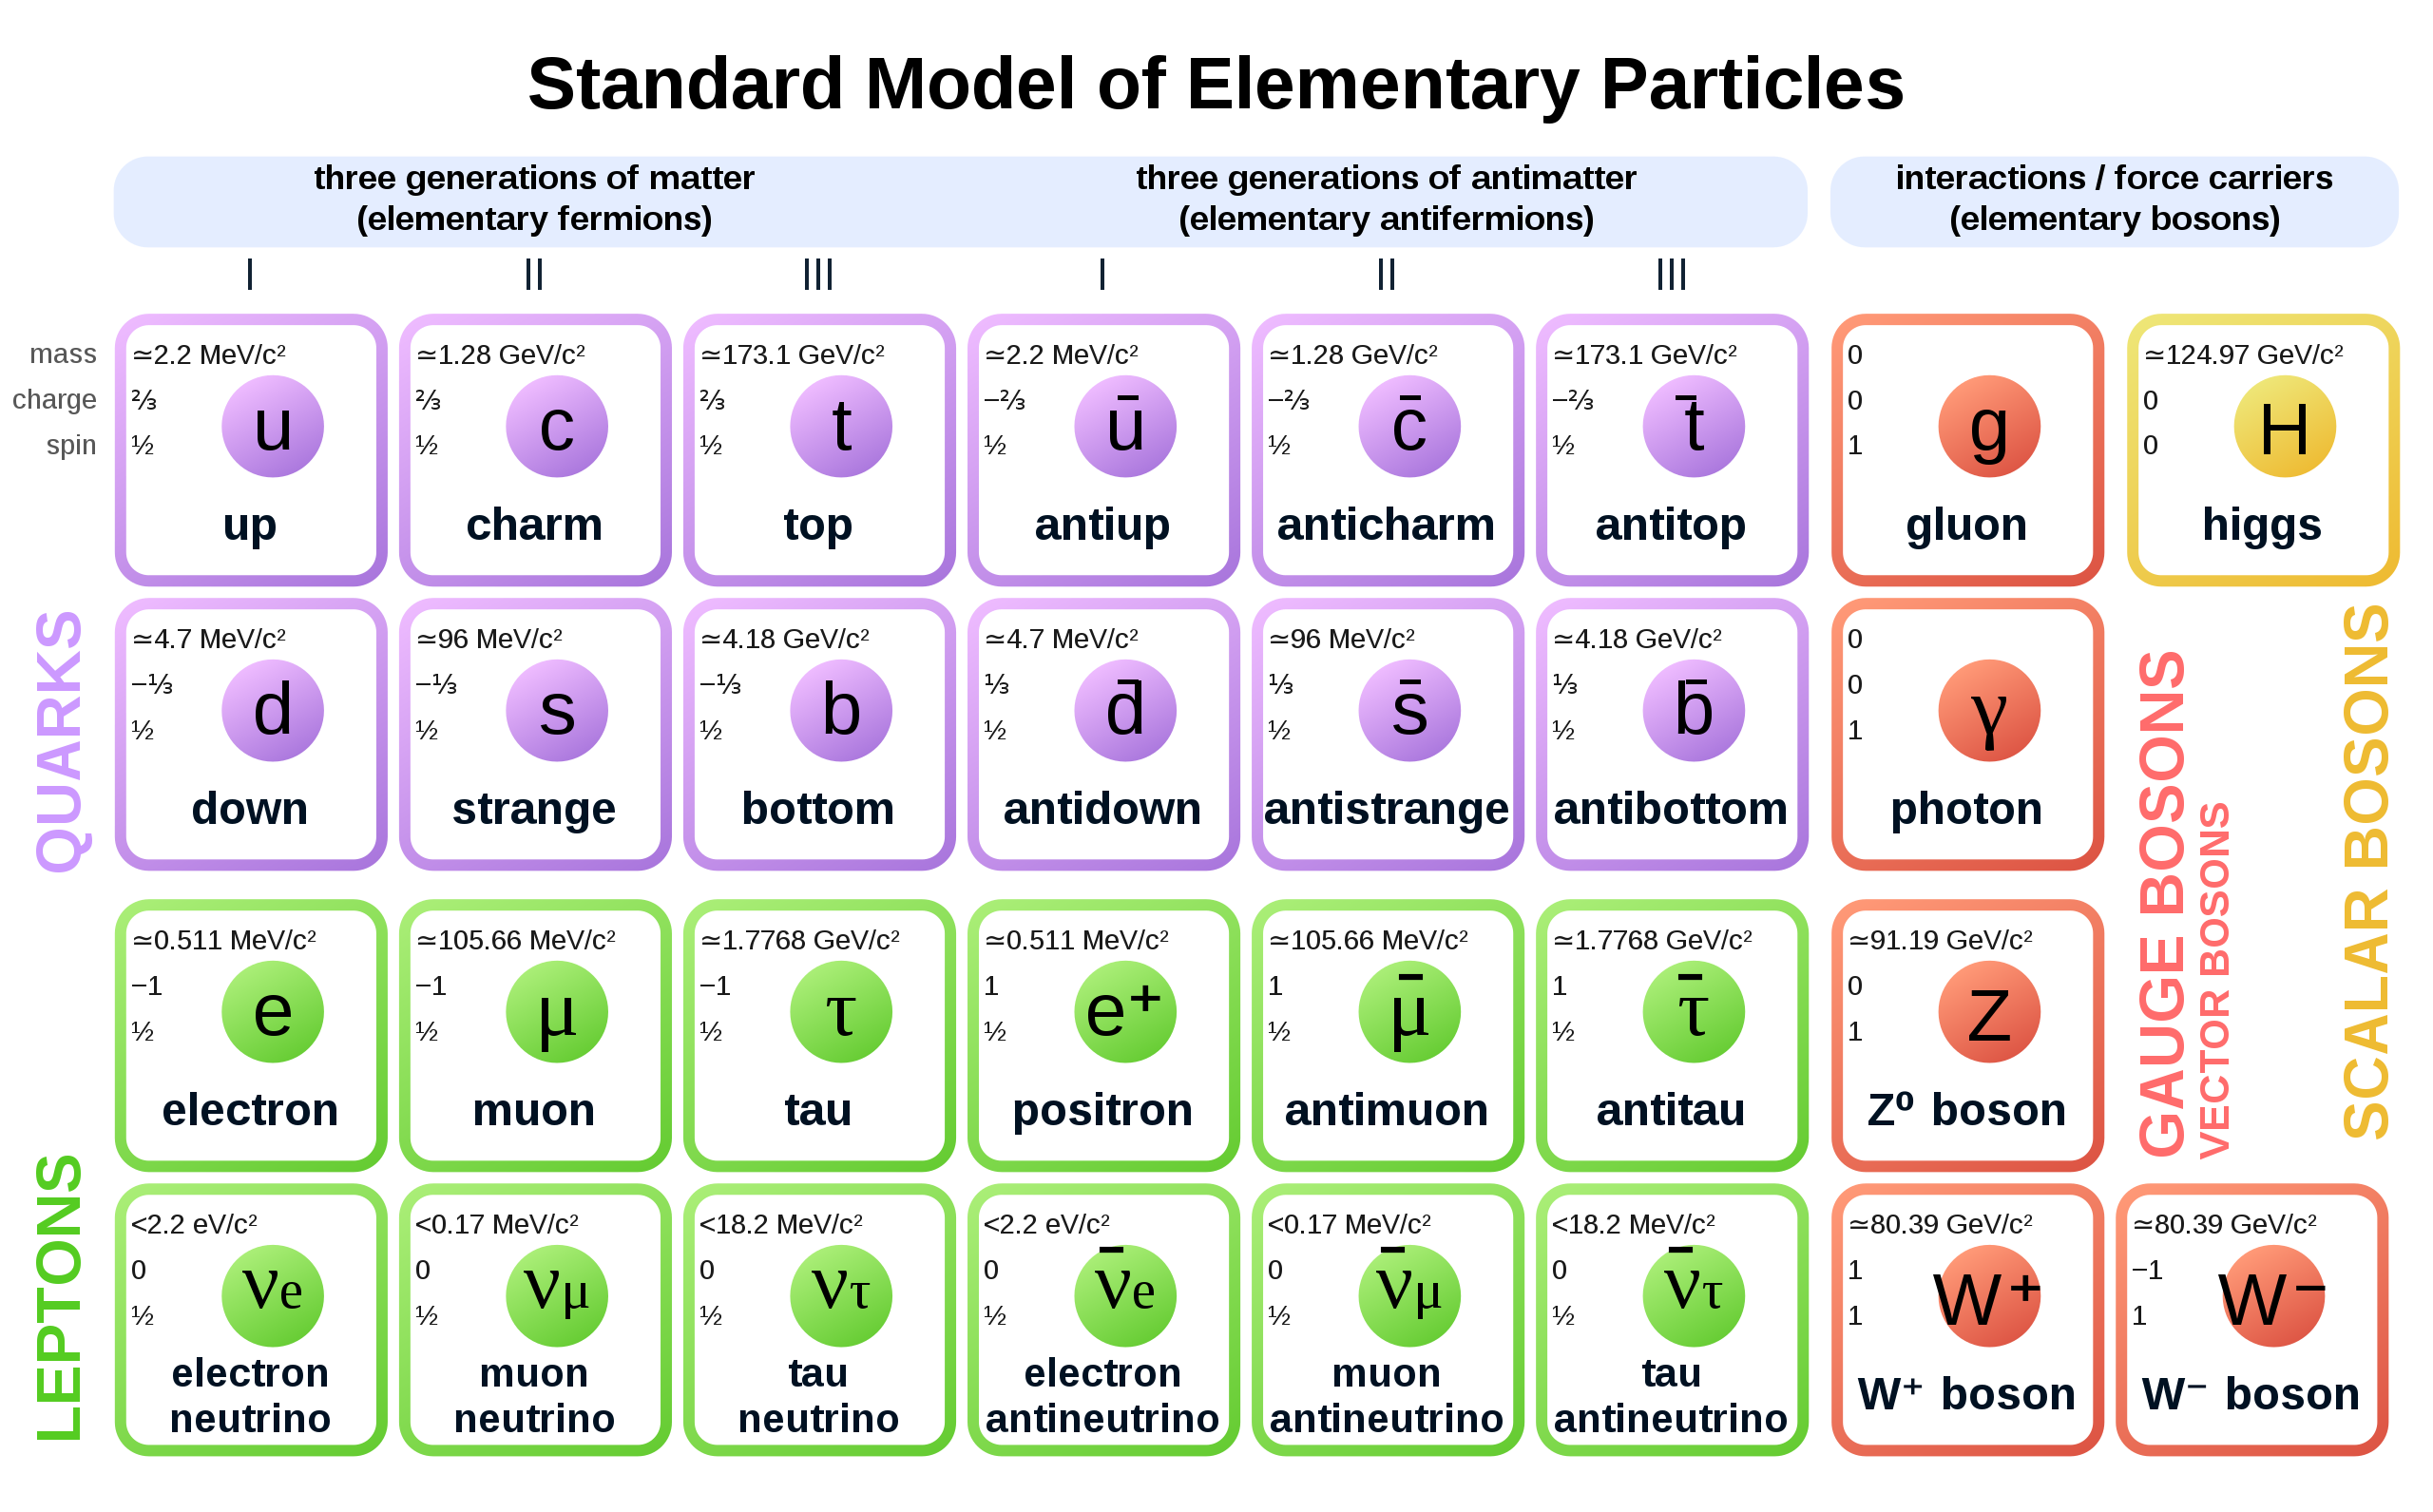
\includegraphics[width=0.99\textwidth]{figures/SMtable.png}
\caption[Summary of standard model fundamental particles]{Summary of SM fundamental particles. Figure source~\cite{SMtable}.
\label{fig:SMParticles}}
\end{figure}


\begin{figure}[t!]
\centering
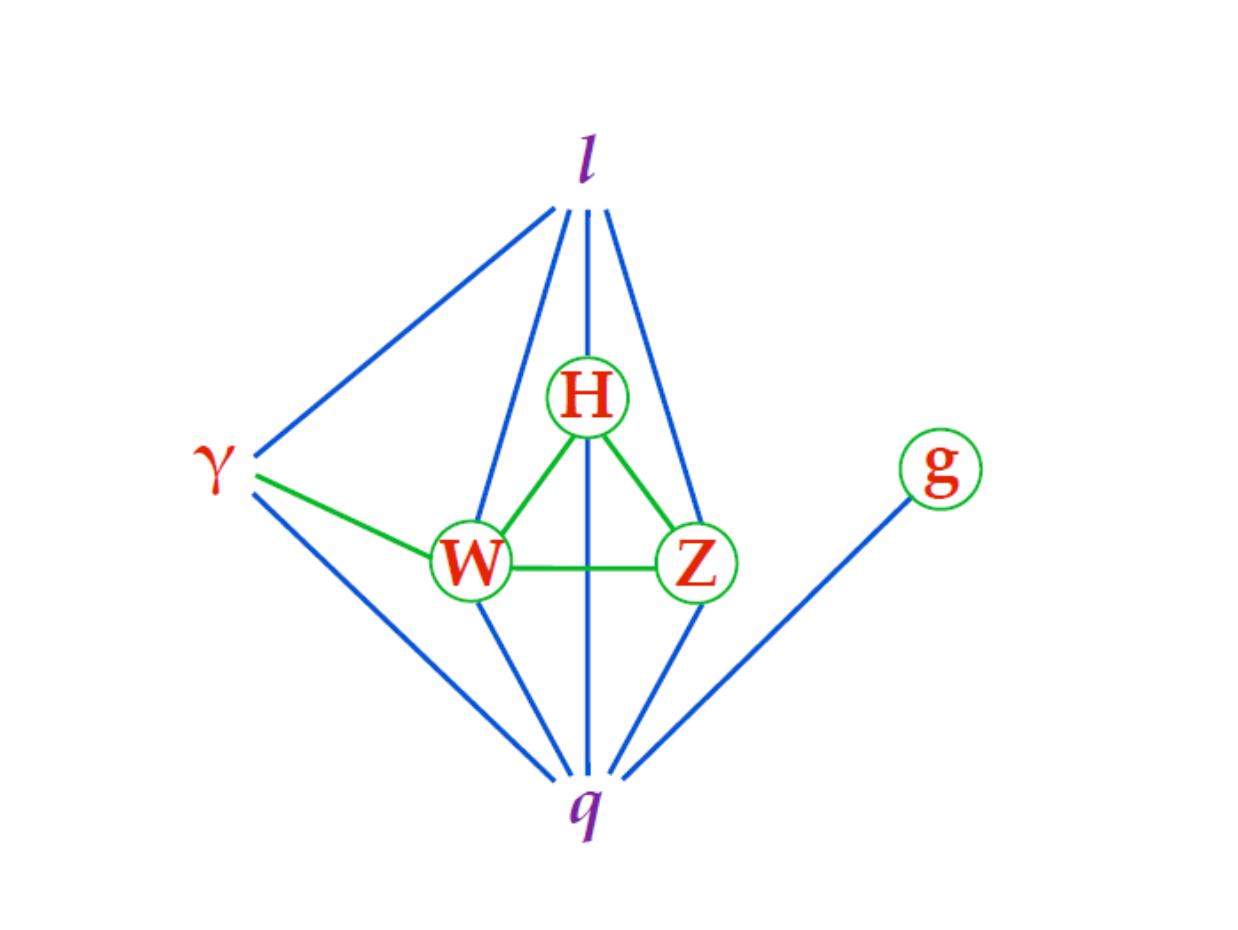
\includegraphics[width=0.99\textwidth]{figures/SM_coupling.png}
\caption[interactions between fundamental particles]
\label{fig:SMcoupling}}
\end{figure}

%
% LHC and experiments, Very brief physics summary
%
The Hadron Collider at CERN, Geneva, Switzerland is currently the largest and highest energy particle accelerator.
The LHC consists of a 27-km ring of superconducting magnets with a number of accelerating structures to boost the energy of the particles along the way.
The LHC can acclerate different types of beams and can produce proton-proton collisions, proton-lead collisions, and lead-lead collisions; however, the main operation mode provides proton-proton collisions.
%
The first proton-proton collisions were achieved by the LHC in 2010 at an energy of 3.5 teraelectronvolts (TeV) per beam, about four times the previous world record.
Over years, the collision energy was inceased and collision rate was also increased.
As of the year of 2024, the LHC collides protons at the center-of-mass energy of $\sqrt{s}=13.6$\TeV.
%
The beams in the LHC cross each other (called bunch crossing) at four points where the ALICE, ATLAS, CMS, and LHCb detectors are located.
%
Since the start of its operation, the experiments at the LHC provide a wide range of physics results and advanced our understanding of elementary particles and their interations.
%
Among various results from LHC experiments, the most signicant one is probably the discovery of the Higgs boson by the ATLAS and CMS experiments~\cite{ATLAS:2012yve,CMS:2012qbp,CMS:2013btf}
in the mass region of around 125\GeV, announced in July, 2012.
%
Since its discovery, the Higgs boson properties have been studied in detailed in different production and decay modes by both ATLAS and CMS experiments.
In addition, all LHC experiments have been making a wide range of measurements to probe elementary particle properties and performing searches for ``new physics`` beyond the SM, and so far no result show significant discrepancies with respect to expectations from the SM.

%
%
%
For these physics studies are not possible without the high performant particle detector.
Among four major LHC experiments, I worked on the CMS experiment.
The CMS detector is described in detail in these references~\cite{CMS,CMS:2023gfb}, and some important aspects are highlighted below.

%
%
%
\section{CMS Detector}

The CMS detector is one of the general purpose detectors at the LHC.
%
Similarly to many other general purpose detectors for hadron collider experiments, the CMS detector consits of multiple subsytems:
the solenoid magnet that bents charged particles, charged particle tracking detector, electromagnetic and hadron calorimeters, and muon detectors.
% Directly taken from
% https://twiki.cern.ch/twiki/bin/viewauth/CMS/Internal/PubDetector
% Long article version.
The central feature of the CMS apparatus is a superconducting solenoid of 6\unit{m} internal diameter, providing a magnetic field of 3.8\unit{T}. Within the solenoid volume are a silicon pixel and strip tracker, a lead tungstate crystal electromagnetic calorimeter (ECAL), and a brass and scintillator hadron calorimeter (HCAL), each composed of a barrel and two endcap sections. Forward calorimeters extend the pseudorapidity coverage provided by the barrel and endcap detectors. Muons are reconstructed in gas-ionization detectors embedded in the steel flux-return yoke outside the solenoid.
The central feature of the CMS apparatus is a superconducting solenoid of 6\unit{m} internal diameter, providing a magnetic field of 3.8\unit{T}.
%
Each of these detector components is described below.

\subsection{Tracker}

The inner tracker measures the momentum of the charged particles by tracking their path going through the magnetic field of the solenoid magnetic.
The less curved the path of the particle the higher its momentum.

The inner tracker tracks the path of the charged particle by measuring its position. The particle produces a tiny signal when passing through the inner tracker layers.
The pixel detector is the closest part of inner tracker to the beam line. It is a crucial component in reconstructing the path of the short-lived particles. It has four cylindrical layers and disks at either end. Each layer is composed of silicon modules  where the sized of pixel is $100\times150$ micrometer$^2$.

The silicon strips cover the pixel detector. Four inner barrel layers (TIB) with two inner endcaps (TID) and six outer barrel layer (TOB) with two endcaps (TED) closing off the tracker. Same as the pixel detector each layer is made of silicon modules that is optimized differently according to its place.

For a charged hadrons at a normal incident with $\pt < 20$\GeV the tracker measures the \pt with 1\% resolution. And the relative resolution will decrease with the increase of \pt to reach the energy resolution of the calorimeter.

\subsection{Superconducting Magnet}

The Superconducting magnet has a strong bending power that can separate the charged from neutral particles energy deposits inside the calorimeters. Also, we can measure the momentum of the charged particles knowing their bend trajectories.This large solenoid magnet covers the inner track and the two calorimeters and provide a $3.8$ T uniform magnetic field on the axial.  

\subsection{Electromagnetic Calorimeter}

The Electromagnetic Calorimeter allows is to measures the energies and the direction of electrons, photons by detecting a cluster of energy which corresponding to electromagnetic showers. The ECAL is a homogeneous calorimeter made of lead tungstate crystals. The crystals in the barrel cover a cylindrical layer while in the endcap they cover an x, y grid. Also, before either endcap disk there is a pre shower detector which serves two goals: finding the photons decayed from a neutral pion to discriminate them from prompt photons. And to by requiring a signal in the pre shower we can indicate the presence of an electron or a photon in the ECAL. The Intrinsic energy resolution of the ECAL barrelis measured with ECAL supermodel exposed to an electron beam. The photon energy resolution is excellent in the range $1-50$ \GeV which is a usual range of photons in jets.  
 

\subsection{Hadronic Calorimeter}

The main function of the HCAL is to detect the energy of the charged and neutral hadrons. A hadronic shower might start in the ECAL which will be fully absorbed in the HCAL. The corresponding clusters in the ECAL and  HCAL will be used to estimate their energies and directions of the hadrons. The HCAL is a sampling calorimeter has layers made of a brass absorber and a plastic scintillator tiles. It covers the ECAL with a barrel and two endcap disks. To extend the coverage Hadron forward calorimeters are placed at $11$ m of the interaction point. The combined (ECAL+HCAL) calorimeter energy resolution was measuredusing a pion test beam. 
 




\subsection{Muon Detector}

What is the main purpose/function of the tracker?
What is the geometry/structure/dimension?
Possibley some purformance measures.

%Here is the introduction to the topic.
%When chapters are referenced, the graduate school requires that words are used rather than numbers, e.g. ``Chapter One'' should be used instead of ``Chapter 1.''
%Use the command \verb|\cref| to reference chapters, for example \verb|\cref{chapter:ch1}|.
%The outline is as follows.
%\cref{chapter:ch2} is about paragraphs and sections.
%\cref{chapter:ch3} discusses footnotes and citations.
%\cref{chapter:ch4} presents floats.
%\cref{chapter:ch5} talks about lists.
%\cref{chapter:ch6} is the conclusion.

\section{The Standrad model}
\label{chapter:ch1}
%intro%

The best theoretical model we currently have that describes all the known fundamental particles and their interactions is known as the standard model theory. 
%The standard model (SM) of particle physics is the best theoretical model we currently have that describes all the known fundamental particles and their interactions.
%This chapter will reviews the basics of the Standrad Model (SM).. (update when the content of chapter is compelet)
The best theoretical model we currently have that describes all the known fundamental particles and their interactions is known as the standard model theory.Particles in the SM can be classified into two categories, as shown in Fig.~\ref{fig:SMParticles}, based on their spin (intrinsic angular momentum) value: fermions have half integer spin, bosons have full integer spin.

Fermions include particles that make up matter this: electrons, protons and neutrons. All fermions follow Pauli exclusion principle which is essential for building atoms and the periodic table. This group of particles can be divided further more into two groups based on the strong force: leptons, do not have strong interactions, and quarks, have strong nuclear interactions.

Quarks cannot be isolated because of the color confinement. They are always found in a bound state known as hadrons interacting via strong force. Hadrons either composed of three quarks, baryons, or a pair of a quark and anti-quark, mesons. Baryons have half integer spin so they are considered fermions while mesons have integer spin so they are considered bosons.

Leptons group consist of three electrically charged particles (electron, muon,and tau) and three electrically neutral neutrinos that come in three flavors associated with the electron, muon, and tau. The electrically charged leptons interact with all forces except for the strong force while neutrinos only interact through gravity and weak force.

Both quarks and leptons can be categorized into
%Each group in quarks  and leptons can be organized into
three generations that differ in their mass.
The heavier generation can decay into the next lighter generation till we reach the lightest one that is stable like (electron, up and  down quarks) (fix me) %“Here insert table that shows these generations”

The force carrying particles in the SM are vector bosons with spin 1. The electromagnetic force is carried by the photon. The strong force is carried by 8 types of gluons. The weak interaction is carried by two charged W bosons and one neutral Z boson. Higgs boson is a scalar boson with spin 0 (that interact with mass?). as shown in Fig.~\ref{fig:SMinteractions}

% note:check if sm details are missing from draft1, also add figures

% include anti matter and how is it associated with matter particles check J.notes purple highlight) 
% use the SM figure
% maybe breifly mention the sectors of SM this is : QCS, EW , strong 
%(consider adding the shortcoming of the SM and how those reasons motivatin the directon of the HEP)
% why SM is incomplete? gravit? 
%..........................     

\begin{figure}[t!]

\centering
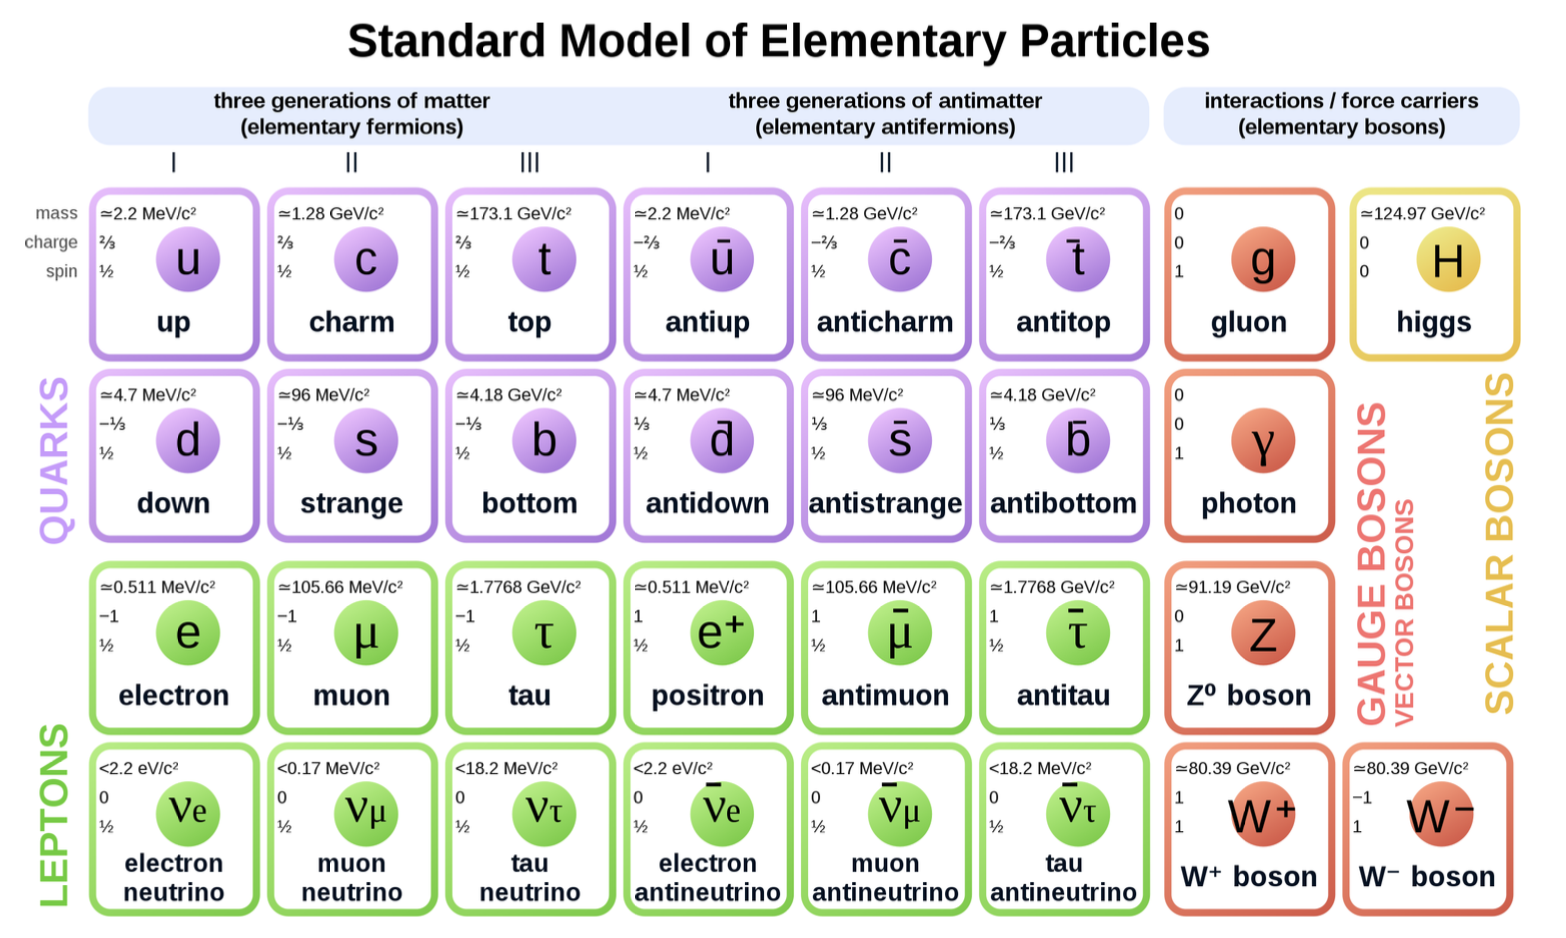
\includegraphics[width=0.99\textwidth]{figures/SM_include_antimatter.png}}
\caption[Summary of standard model fundamental particles]{Summary of SM fundamental particles. Figure source~\cite{SMtable}.
\label{fig:SMParticles}}

\end{figure}

\begin{figure}[t!]
\centering
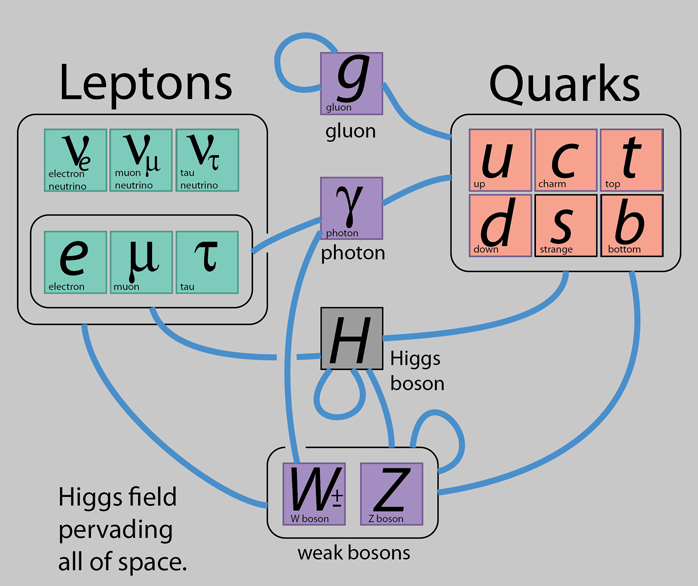
\includegraphics[width=0.50\textwidth]{figures/interactions_SM.png}}
\caption[Summary of standard model fundamental particles]{Summary of SM fundamental particles. Figure source~\cite{SMintera}.
\label{fig:SMinteractions}}
\end{figure} 


\section{The large hadron collide}
\label{chapter:ch2} 

% intro %

In high	energy physics, we need two things: acceletors to create particles and detectors to detect them. LHC is one of the biggest acceleratos we have today, and one on if its general detectors is (CMS) which is related to this thesis.This chapter provides details about LHC, protons journey at LHC, and discribtion of CMS detector.   

%................................
%\section{The large hadron collide}

The large hadron collider is the most powerful particle accelerator in the world. From its name “Large” refer to its big size which is about 27km in circumference and “Hadron" because it accelerates particles like protons or ions which are known as hadrons.Lastly, "Collider" because the particles traveling into two beams in opposite directions, are made to collide at four points around LHC ring.

The LHC is a part of the CERN accelerator complex and sits in a tunnel 100 meters underground at CERN, the European Organization for Nuclear Research, on the border of Switzerland and France near Geneva, Switzerland.

The CERN accelerator complex is a succession of machines where each machine accelerates a beam of particles to a given energy before injecting the beam into the next machine in the chain. LHC is the last element of this chain where it is designed to collide particles at COM energy up to 14 TeV.

The LHC is made of eight arcs and eight ‘insertions. The arcs contain the dipole ‘bending’ magnets. The layout of the straight section depends on the specific use of the insertion: physics (beam collisions within an experiment), injection, beam dumping or beam cleaning.

At the LHC we have 9 experiments:
ALICE (study heavy ion collisions, QGP) ATLAS, CMS  (general purpose detectors) LHCb (study matter – antimatter asymmetry) ,LHCf (shares intersection with ATLAS),TOTEM (shares intersection with CMS) MoEDAL-MAPP, (shares intersection with LHCb), FASER,SND@LHC.

\subsection{The journey of protons in the LHC}

It all starts from a compressed tank of hydrogen that is connected to source chamber of the linear accelerator.
The Linear accelerator 4 (Linac4) is designed to boost negative hydrogen ions (H with extra electron) to high energies (initial to 1/3 C).Then the particles are fed to the booster stage. (Proton Synchrotron Booster – PSB).at the PSB injection point a stripping foil will strip the electrons off the hydrogen anions creating protons that are accumulated as beam bunches in the four PSB rings.

These proton bunches are then recombined at the exit of the PSB and further transferred down theCERN injector chain (accelerated to 91.6 of C).After that the beam is sent to Proton synchrotron (PS) where the increase of energy does not transfer to velocity.
Instead, it will increase the relativistic mass (accelerated to 99.9 of C).

Then the protons go to the super proton synchrotron. (SPS). Finally, at the LHC has two vacuum pipes where the protons will be going into different directions. 27 km ring of superconducting magnets (keep protons in the ring) that also has  accelerating structures (radio frequency cavities) to boost the energy. The LHC’s RF cavities bring the 450 GeV energy  of the particles (1 GeV = 1 billion electron volts) to 6.5 TeV source.

The maximum energy is reached in around 20 minutes with the bunches having passed through the RF cavities more than 10 million times.There are 4 points where the protons are collided. CMS is one of the them, where this thesis is focus on.

\section{CMS Detector}

CMS detector is one of the main detectors at the LHC. It is a general-purpose detector. its physics program rang from studying the Standard Model (including the Higgs boson) to searching for extra dimensions and particles that could make up dark matter.
CMS stands for Compact Muon Solenoid. measure the position and energy of all particles that comes from the collision. This detector weights 14,000-tonne but it is quite compact for all the detector material it contains. It is at 15 m high  and 21 m long.
CMS is it isdesigned to detect muons very accurately. Also, it has the most powerful solenoid magnet ever made.

The design of CMS and its subdetectors are based on the geometry of its solenoid magnet. some of the subdetectors are located inside the magnet while the rest are outside the magnetic field. Inside starting from the closest to the beam pipe we have: Silicon tracker (Silicon pixel, Silicon strips) designed to minimally interact with particles. ECAL & HCAL will stop and absorb the particles completely (calorimeters).  Outside the magnet there are some of HCAL subdetectors a\
nd muon systems.


\subsection{Superconducting Magnet}
It is superconducting magnet that produces 3.8 T magnetic field inside a solenoid and quickly drops off outside it. Thi\
s magnetic field is used to determine the momenta of charged particles since the trajectories of the particles bend in \
the field.

\subsection{Inner Tracker}
the first subdetector particles created from the collision will interact with after leaving the beam pipe is the tracker. The most inner parts of the CMS detector are: the pixels, silicon microstrip detectors that surrounds the pixels.

Main function of the tracker is to measure the curvature of charged particles with pt > 1 GeV. From which we can use to determine the momentum. When a charged particle goes through the tracker it will leave a hit (tiny signal that will later be amplified and detected) in the tracker layers. These hits could be aligned to get the trajectory of the particle. The signals will be stored for microseconds and then processed before being sent to a laser to be converted to an infrared pulse Which will be transmitted for analysis.

The pixel detector:
It is also the closest detector to the beam pipe. It has 4 cylindrical layers at (3,7,11,16 cm) . Each of the four layers is composed of individual silicon module (? How many), splitted into little silicon sensors (pixels).  Each of these silicon pixels is 100µm by 150µm.

The silicon strips
After the pixels the particles go through the silicon strip detector, which has10 layers. (130 cm~ 1.3m). 4 inner barrel layers (TIB) with two inner endcaps (TID) each has 3 small disks. Then we have 6 outer barrel layer (TOB) surrounds both TIB, TID with two endcaps (TED) closing off the tracker. this part contains 15,200 highly sensitive modules with a total of about 10 million detector strips.

(insert real/sketch updated picture of each subdetector)


\subsection{Electromagnetic Calorimeter}
it is a homogeneous calorimeter made of lead tungstate crystals. Measures the energy of electrons and photons. It is made up of a “barrel” section and two “endcaps”, that would form a layer between the tracker and the HCAL.
tungstate crystals are heavier than stainless steel but it is transparent. It scintillates when electrons and photons pass through it. Which will produce light that is that is proportion to the particle energy.

glued onto the back of each of the crystals a Photodetectors, which have been especially designed to work within the high magnetic field, will detect the scintillation light and convert it to an electrical signal that is amplified and sent for analysis.

The barrel region: consists of 61,200 crystals formed into 36 “supermodules”, each weighing around three tonnes and con\
taining 1700 crystals. Here each crystal (2.2 x 2.2 x 23 cm). it can contain more than 98 of the electrons and photons \
energy.

The endcap regions close off the barrel at each end and are made  up of almost 15,000 more crystals. each crystal (3 x 3\
 x 22 cm) which corresponding to 24.7 radiation lengths. For more precision, the ECAL also contains a pre shower detector that is Finer grained detector and located before either endcap disk.  has two layers, each layer is made of two orthogonal layers of silicon sensors, interspersed with lead layers that serve to generate electromagnetic showers. This detector serves two goals Find the photons decaying form a neutral pion to discriminate them from prompt photons.  Indicate the presence of an electron or a photon in the ECAL be requiring a related signal in the pre shower.


 (what pics to include?)

 \subsection{Hadronic Calorimeter}

 Hermetic & sampling calorimeter
It is “hermetic” makes sure it captures, to the extent, every particle emerging from the collisions. It HCAL measures directly the energy of “hadrons”. Like: neutrons, Pions and kaons and indirect the presence of non-interacting, uncharged particles such as neutrinos by seeing the imbalance in the momentum and energy (measured in the sideways “transverse” direction relative to the beam line).

HCAL is also a sampling calorimeter made of alternating layers of “absorber” (dense material - brass or steel) and fluo rescent “scintillator” (tiles of plastic) that produce a rapid light pulse when the particle passes through.
the HCAL is organized into: Barrel region: (HB) these form the last layer of detector inside the magnet coil while a few additional layers the outer barrel (HO), sit outside the coil, ensuring no energy leaks out the back of the HB undetected. endcap regions measure particle energies as they emerge through the ends of the solenoid magnet. Forward sections  positioned at either end of CMS; to pick up the myriad particles coming out of the collision region at shallow angles relative to the beam line, these receive the bulk of the particle energy contained in the collision so they must be very resistant to radiation and use different materials to the other parts of the HCAL.

When a hadronic particle hits a plate of absorber, in this case brass or steel, an interaction can occur producing numerous secondary particles. As these secondary particles flow through successive layers of absorber. they too can interact and a cascade or “shower” of particles results.

As this shower develops, the particles pass through the alternating layers of active scintillation material causing the\
m to emit blue-violet light. Within each tile tiny optical absorb this light. clear optic cables then carry the light a\
way to readout boxes located at locations within the HCAL volume. signals from successive tiles, one behind the other, \
are added optically to form “towers”. These summed optical signals are converted into fast electronic signals by photos\
ensors.

(insert sketch that shows the subdetectors of the HCAL)

\subsection{Muon Detector}
Detecting muons is one of CMS’s most important tasks. unlike most particles muons are not stopped by any of CMS’s calorimeters.That is why chambers to detect muons are placed atthe very edge of the experiment where they are the only particles likely to register a signal.muon chambers that include: Drift tubes (DTs) and cathode strip chambers (RPCs) are arranged in concentric cylinders around the beam line in the barrel region. In endcap region we have CSCs and resistive plate chambers (RPCs) which make u\
p the “endcaps” disks that cover the barrel (add gas electron multiplier chambers (GEMs))
the muon is measured by fitting a curve to hits among the four muon stations (MS) which sit outside the magnet coil and\
 are interleaved with iron “return yoke” plates.
 (Insert picture that shows the placement of each type in both regions)

 


 %------------ figures ------------%
\begin{figure}[t!]
\centering
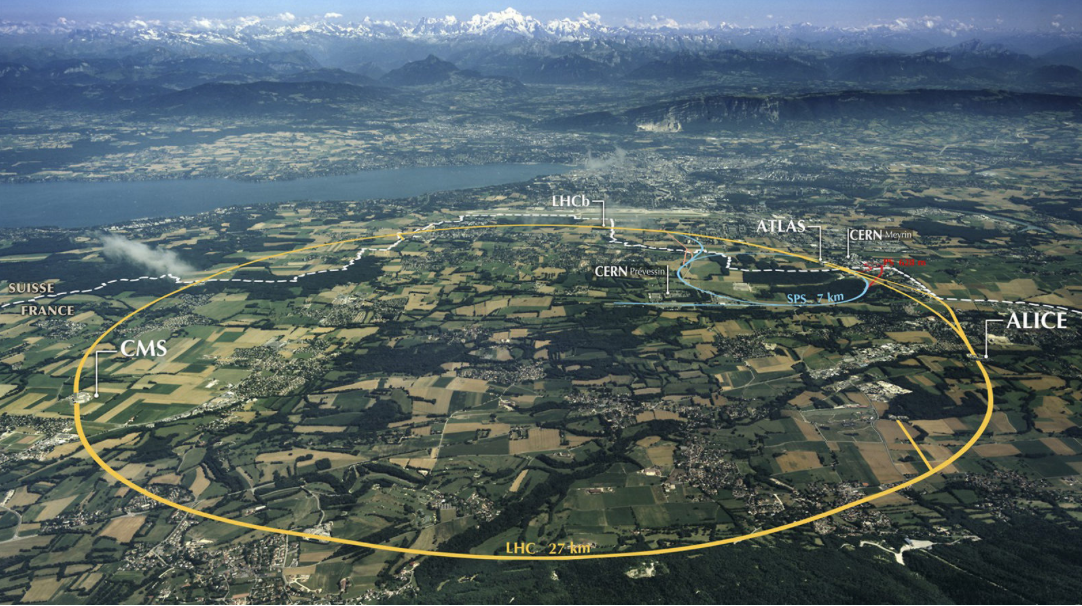
\includegraphics[width=0.99\textwidth]{figures/LHC_location.png}}
\caption[location of the LHC]{}. Figure source~\cite{SMtable}.
\label{fig:SMParticles}}
\end{figure}

\begin{figure}[t!]
\centering
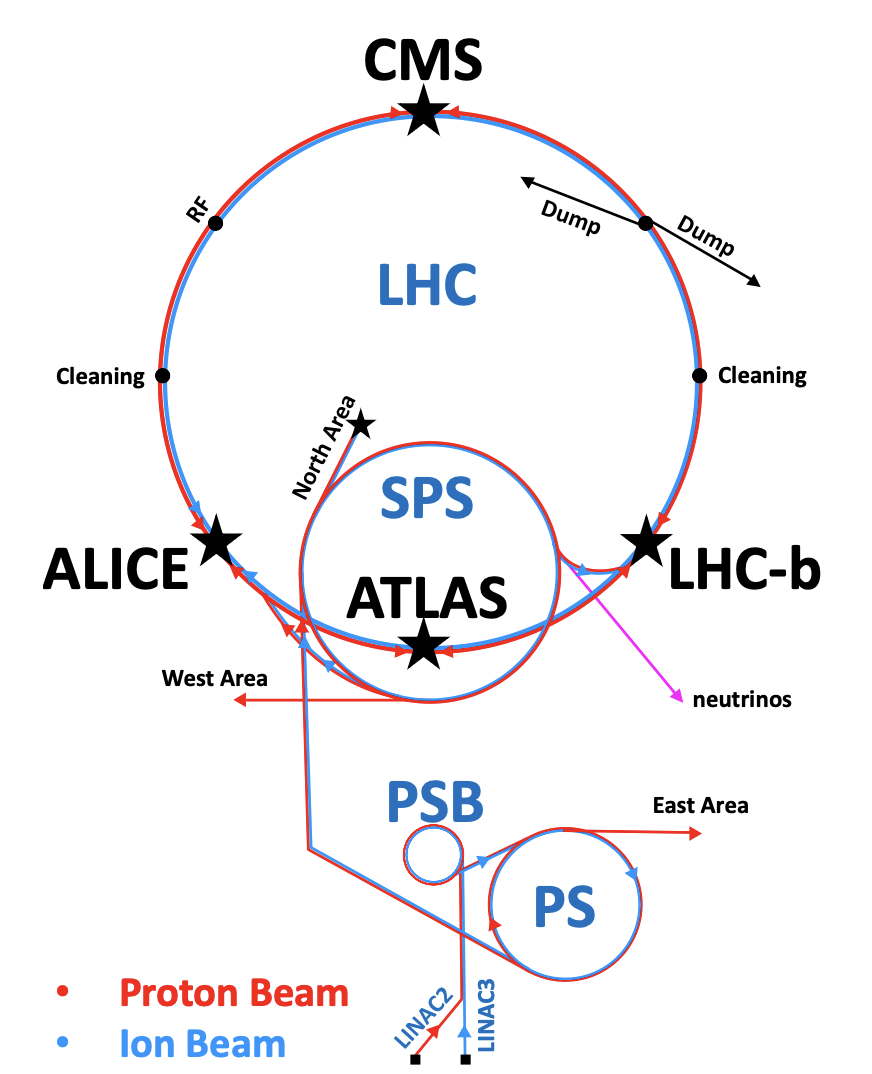
\includegraphics[width=0.99\textwidth]{figures/acceleration_chain.png}}
\caption[acceleration complex]{}. Figure source~\cite{SMtable}.
\label{fig:SMParticles}}
\end{figure} 
   


%\section{The CMS experiment}
%\label{chapter:ch3}

\section{Particle Flow Algorithm}
\label{chapter:ch4}
A% how to would explain PF to someone who doesnot know anything about HEP %

When we collide particles at high energies inside a particle detector, the collision products either will decay into a final stable particle that can be detected or
it  would not interact with the detector. 

(collision products could be: a heavy particle that decays into a stable particle like tau,
or jet of long lived particles (charged hadrons, photons from neutral pions, neutral hadrons) produced when a quark/gluon hadronizes,
or particles that don't intereact with the detector like neutrinos) (source?) 

To able to see the products orginated from collision, we need a way to reconstruct them from the stable particles captured by the detector.
CMS experiments is able to do that using a reconstruction alogrithm called particle flow (PF).

This alogorithm uses the various signals captured by the CMS subdetectors to derive physics objects originated from the collision (like:Muons, electrons, photons, jets, taus, missing transverse energy)
which will be stored for further analysis in the future.

This chapter will proivde a breif description of PF algortihm, calorimeter clusters. Additionally, calibration cluster calibration which is related to work done in this thesis.  

%\section{Particle Flow Reconstruction}

as mentioned previously, The PF algorithm aims to reconstruct and identify all final particles produce in the event (what do mean by an event?).
This is achieved by utilizing the fact that different particles leave different signatures in the CMS subdetectors.

we have two types of PF reconstruction. Online whichs is required to be done quickly during data taking to select interesting events (what kind of events we are looking for?) , it is not integrated in the PF framework (clear this point, what is the PF framework? ) .
and offline which tht is done after data is collected. it takes more time to achieve higher precision. algorithms, for clustering and tracking, are integrated in the PF framework.

(in ECAL chapter we cover HLT PF cluster claibraton)

The PF algrithm is done in multiple steps.
it starts with reconstructing the basic elements of the PF: tracks, energy clusters which are using advanced algorithm.
The details of the clustering algorithm and the calibration of the clusters will be discussed in the next sections.

Then forming links between the PF elements based on their spatial proximity.
(the linking rule is to cannect a small thing a big one where they must be touching in the eta-phi space)
(the order of the size from small to big track<Ecal<Hcal)
(links could be formed between tracks and ECAL cluster, tracks and HCAL clusters, ECAL and HCAL clusters, inner tracks and muon tracks, muon tracks and ECAL clusters, muon tracks and HCAL clusters)

after all the links are established, PF blocks are formed from all groups of linked tracks and clusters.  
(note we could have blocks from the an alone elemet like a single track or a cluster) 
(insert skitch of the blocks) 
% source intro to PF workshop

the final step in the PF is to derive the list of PF particle candidate from the PF blocks.
this decison is done by following a stric order. after checking the tracks and clusters associated to a PF cadidate, they will be removed from their blocks.

this order starts with the cleanest signture in the CMS muons. Then, isolated electrons and photons (ECAL clusters not linked to HCAL cluster).
Then neutral hadrons and photons (all left clusters without track link) (Ecal cluster will be assigned to photon candidates and HCAl clusters will be assigned to a neural hadron)
after that everything left are charged hadrons.

for charged hadrons, the energy must be calibrated. this could be done by comparing the sum of cluster energy to the sum of the track momenta.
(expand more on the calibration done here, in case overlap of charged and neutral hadron)
(also any alone tracks will be assigned as charge hadrons)

\subsection{Calorimeter Clustering}

Clustering in done in each calorimeter following three steps.
First, we need to identify topological clusters and their seeds. After that we can compute cluster positions and energies.

We can identify topological clusters by looking for a group of calorimeter cells, each has energy deposit above a certain threshold, that share at least one neighbor.
Then we identify any calorimeter cell whose energy is a local maximum, with respect to its immediate neighbors, this is a seed.
Topological clusters must have one seed or multiple.

When Computing cluster positions and energies we have two kinds of topological clusters.
One with Single-seed and the other type has Multiple-seed.

In the Single-seed case the cluster energy will be the sum of all the individual cell energies within the cluster and its position is going to be the energy-weighted average of the individual cell positions.

For Multiple-seed case, each seed is assumed to represent a unique energy cluster,but the energy deposited in non-seed cells will be shared between the various clusters within the topological cluster.
An iterative procedure is used to converge on cluster energies and positions based on energy-weighted averages of fractional cell energies.
(we could include eq that shows how the energy is shared between the seeds or add a skitch)

\section{Cluster Calibration}

as seen in PF section, photons and neutral hadrons are reconstructed only from calorimeter clusters.
and charged hadrons can be calibrated by check the track momenta.

an accurate calibration of the calorimeter response to photons and hadrons is important to maximize the probability to identify the neutral particles and
also to minimize the rate of misreconstructed energy excesses.
% source: PF paper pg 16 

\subsection{ECAL Cluster Calibration}

(mention calibration done before data taking breif) 
(here correction is mostly due to thresholds) 

(will add soon)	

\subsection{HCAL Cluster Calibration}

(hadrons could start showering in the ECAL)
(from previous section, ECAL is calibrated well for EM components but not for hadrons)

(will add soon)	
 

%=====================================
%\chapter{The LHC and the CMS experiment}
%\chapter{Introduction}
%\label{chapter:ch3}
%%%outline%% ECAL Cluster Calibration using Boosted Decision Tree

intro..
 talk about ECAL.
 introduce clustering algorithm in ECAL.  
 HLT vs offline PF ECAL cluster
 
 expand more on:
  the PF cluster calibration.
  how it was done perviously, and now in this thesis. 
  
computational details.. 
 3.1 Boosted Decision Tree (BDT)
  based semi-parametric regression.

 3.2 BDT training details  
  samples being used. for training and validation.
  Calibration procedure. Input and target variables to BDT.

 3.3 fitting function 
 Crystal Ball (CB) double function
 
Results and Discussion (might be moved to its chapter before conclusion) 
 compare old vs new corrections
 check the response, resolution in each regions EE. EB. add comments if the results has improved or stayed the same. 

%plots : showing (EB , EE regions) 
%-  mu vs pt (covering 3 ranges of pt gen particle) (EB , EE regions)
%-  mu vs eta (for each range of pt) (EB region)


\begin{figure}[ht]
%\centering
%\includegraphics[width=1in]{baylor}
\caption{EB - Full Readout : mu vs eta}
%\label{figure_example1}
\end{figure} 

\begin{figure}[ht]
%\centering
%\includegraphics[width=1in]{baylor}
\caption{EE - Full Readout : mu vs eta}
%\label{figure_example1}
\end{figure}

\begin{figure}[ht]
%\centering
%\includegraphics[width=1in]{baylor}
\caption{EB - Full Readout : mu vs pt}
%\label{figure_example1}
\end{figure}

\begin{figure}[ht]
%\centering
%\includegraphics[width=1in]{baylor}
\caption{EE - Full Readout : mu vs pt}
%\label{figure_example1}
\end{figure}

Include some set of stamp plots. (where we get mu & std from after fitting)

Now, for ZS set vs pt.

%\includegraphics[width=1in]{baylor}
\caption{EE - ZS Readout : mu vs pt}
%\label{figure_example1}
\end{figure}

\begin{figure}[ht]
%\centering
%\includegraphics[width=1in]{baylor}
\caption{EB - ZS Readout : mu vs pt}
%\label{figure_example1}
\end{figure}

HLT vs offline PF ECAL cluster

%1-plots :
%- (PF cluster offline E / PFC online E) vs pt
%- (PF cluster offline E / PFC online E) vs eta
%%%%%%%%%%%%%%%%%%%%%%%%%%%%%%%%%%%%%%%%%%%%%%%
\begin{figure}[ht]
%\centering
%\includegraphics[width=1in]{baylor}  
\caption{(PF cluster offline E / PFC online E) vs pt}
%\label{figure_example1}
\end{figure}

\begin{figure}[ht]
%\centering
%\includegraphics[width=1in]{baylor}
\caption{(PF cluster offline E / PFC online E) vs eta}
%\label{figure_example1}
\end{figure}
%%%%%%%%%%%%%%%%%%%%%%%%%%%%%%%%%%%%%%%%%%%%%%%%
%plots : 
%- (PF cluster offline corrected E / PFC online corrected  E) vs pt
%- (PF cluster offline corrected E / PFC online corrected  E) vs eta 
%%%%%%%%%%%%%%%%%%%%%%%%%%%%%%%%%%%%%%%%%%%%%%%
\begin{figure}[ht]
%\centering                                                                                                                                                                                                                                                                     
%\includegraphics[width=1in]{baylor}                                                                                                                                                                                                                                            
\caption{(PF cluster offline corrected E / PFC online corrected E) vs pt}
%\label{figure_example1}                                                                                                                                                                                                                                                        
\end{figure}~

\begin{figure}[ht]
%\centering 
%\includegraphics[width=1in]{baylor}
\caption{(PF cluster offline corrected E / PFC online corrected E) vs eta}
%\label{figure_example1}
\end{figure}~
%%%%%%%%%%%%%%%%%%%%%%%%%%%%%%%%%%%%%%%%%%%%%%%%

\section{Footnotes}

Ut vitae elit blandit, dictum augue aliquam, dictum neque. Integer sit amet eros
iaculis, interdum est quis, convallis metus. Maecenas vestibulum id lectus at
pellentesque.\footnote{This is a short footnote.} Aliquam dignissim, turpis eget
hendrerit ullamcorper, magna magna consectetur odio, pulvinar vestibulum felis
enim in ipsum. Donec cursus pharetra fringilla. Integer placerat ultrices libero
non porta. In id orci in ipsum aliquet rhoncus. Fusce ornare ornare
volutpat.\footnote{And this is a rather longer footnote that requires more than
one line, demonstrating the required single spacing.}

Vivamus vel tortor vel nibh aliquet egestas. Nullam rutrum porttitor placerat.
Pellentesque mattis ullamcorper sollicitudin. Nam et arcu nisi. Aenean hendrerit
odio non nisi ultricies, in consectetur odio rhoncus. Donec cursus consequat
tincidunt. Morbi pellentesque ut sem sit amet sollicitudin. Quisque bibendum
tincidunt quam, eu condimentum dui ullamcorper at.

\section{Citations}

Here is a citation \cite{fake1}, and here is another \cite{fake2}. Citations are
nice. Depending on your choice of bibliography, there may be different formats
you can use. For example, Chicago provides a family of short citation commands.

%\label{chapter:ch2}
%
% intro %

In high	energy physics, we need two things: acceletors to create particles and detectors to detect them. LHC is one of the biggest acceleratos we have today, and one on if its general detectors is (CMS) which is related to this thesis.This chapter provides details about LHC, protons journey at LHC, and discribtion of CMS detector.   

%................................
\section{The large hadron collide}

The large hadron collider is the most powerful particle accelerator in the world. From its name “Large” refer to its big size which is about 27km in circumference and “Hadron" because it accelerates particles like protons or ions which are known as hadrons.Lastly, "Collider" because the particles traveling into two beams in opposite directions, are made to collide at four points around LHC ring.

The LHC is a part of the CERN accelerator complex and sits in a tunnel 100 meters underground at CERN, the European Organization for Nuclear Research, on the border of Switzerland and France near Geneva, Switzerland.

The CERN accelerator complex is a succession of machines where each machine accelerates a beam of particles to a given energy before injecting the beam into the next machine in the chain. LHC is the last element of this chain where it is designed to collide particles at COM energy up to 14 TeV.

The LHC is made of eight arcs and eight ‘insertions. The arcs contain the dipole ‘bending’ magnets. The layout of the straight section depends on the specific use of the insertion: physics (beam collisions within an experiment), injection, beam dumping or beam cleaning.

At the LHC we have 9 experiments:
ALICE (study heavy ion collisions, QGP) ATLAS, CMS  (general purpose detectors) LHCb (study matter – antimatter asymmetry) ,LHCf (shares intersection with ATLAS),TOTEM (shares intersection with CMS) MoEDAL-MAPP, (shares intersection with LHCb), FASER,SND@LHC.

\subsection{The journey of protons in the LHC}

It all starts from a compressed tank of hydrogen that is connected to source chamber of the linear accelerator.
The Linear accelerator 4 (Linac4) is designed to boost negative hydrogen ions (H with extra electron) to high energies (initial to 1/3 C).Then the particles are fed to the booster stage. (Proton Synchrotron Booster – PSB).at the PSB injection point a stripping foil will strip the electrons off the hydrogen anions creating protons that are accumulated as beam bunches in the four PSB rings.

These proton bunches are then recombined at the exit of the PSB and further transferred down theCERN injector chain (accelerated to 91.6 of C).After that the beam is sent to Proton synchrotron (PS) where the increase of energy does not transfer to velocity.
Instead, it will increase the relativistic mass (accelerated to 99.9 of C).

Then the protons go to the super proton synchrotron. (SPS). Finally, at the LHC has two vacuum pipes where the protons will be going into different directions. 27 km ring of superconducting magnets (keep protons in the ring) that also has  accelerating structures (radio frequency cavities) to boost the energy. The LHC’s RF cavities bring the 450 GeV energy  of the particles (1 GeV = 1 billion electron volts) to 6.5 TeV source.

The maximum energy is reached in around 20 minutes with the bunches having passed through the RF cavities more than 10 million times.There are 4 points where the protons are collided. CMS is one of the them, where this thesis is focus on.

\section{CMS Detector}

CMS detector is one of the main detectors at the LHC. It is a general-purpose detector. its physics program rang from studying the Standard Model (including the Higgs boson) to searching for extra dimensions and particles that could make up dark matter.
CMS stands for Compact Muon Solenoid. measure the position and energy of all particles that comes from the collision. This detector weights 14,000-tonne but it is quite compact for all the detector material it contains. It is at 15 m high  and 21 m long.
CMS is it isdesigned to detect muons very accurately. Also, it has the most powerful solenoid magnet ever made.

The design of CMS and its subdetectors are based on the geometry of its solenoid magnet. some of the subdetectors are located inside the magnet while the rest are outside the magnetic field. Inside starting from the closest to the beam pipe we have: Silicon tracker (Silicon pixel, Silicon strips) designed to minimally interact with particles. ECAL & HCAL will stop and absorb the particles completely (calorimeters).  Outside the magnet there are some of HCAL subdetectors a\
nd muon systems.


\subsection{Superconducting Magnet}
It is superconducting magnet that produces 3.8 T magnetic field inside a solenoid and quickly drops off outside it. Thi\
s magnetic field is used to determine the momenta of charged particles since the trajectories of the particles bend in \
the field.

\subsection{Inner Tracker}
the first subdetector particles created from the collision will interact with after leaving the beam pipe is the tracker. The most inner parts of the CMS detector are: the pixels, silicon microstrip detectors that surrounds the pixels.

Main function of the tracker is to measure the curvature of charged particles with pt > 1 GeV. From which we can use to determine the momentum. When a charged particle goes through the tracker it will leave a hit (tiny signal that will later be amplified and detected) in the tracker layers. These hits could be aligned to get the trajectory of the particle. The signals will be stored for microseconds and then processed before being sent to a laser to be converted to an infrared pulse Which will be transmitted for analysis.

The pixel detector:
It is also the closest detector to the beam pipe. It has 4 cylindrical layers at (3,7,11,16 cm) . Each of the four layers is composed of individual silicon module (? How many), splitted into little silicon sensors (pixels).  Each of these silicon pixels is 100µm by 150µm.

The silicon strips
After the pixels the particles go through the silicon strip detector, which has10 layers. (130 cm~ 1.3m). 4 inner barrel layers (TIB) with two inner endcaps (TID) each has 3 small disks. Then we have 6 outer barrel layer (TOB) surrounds both TIB, TID with two endcaps (TED) closing off the tracker. this part contains 15,200 highly sensitive modules with a total of about 10 million detector strips.

(insert real/sketch updated picture of each subdetector)


\subsection{Electromagnetic Calorimeter}
it is a homogeneous calorimeter made of lead tungstate crystals. Measures the energy of electrons and photons. It is made up of a “barrel” section and two “endcaps”, that would form a layer between the tracker and the HCAL.
tungstate crystals are heavier than stainless steel but it is transparent. It scintillates when electrons and photons pass through it. Which will produce light that is that is proportion to the particle energy.

glued onto the back of each of the crystals a Photodetectors, which have been especially designed to work within the high magnetic field, will detect the scintillation light and convert it to an electrical signal that is amplified and sent for analysis.

The barrel region: consists of 61,200 crystals formed into 36 “supermodules”, each weighing around three tonnes and con\
taining 1700 crystals. Here each crystal (2.2 x 2.2 x 23 cm). it can contain more than 98 of the electrons and photons \
energy.

The endcap regions close off the barrel at each end and are made  up of almost 15,000 more crystals. each crystal (3 x 3\
 x 22 cm) which corresponding to 24.7 radiation lengths. For more precision, the ECAL also contains a pre shower detector that is Finer grained detector and located before either endcap disk.  has two layers, each layer is made of two orthogonal layers of silicon sensors, interspersed with lead layers that serve to generate electromagnetic showers. This detector serves two goals Find the photons decaying form a neutral pion to discriminate them from prompt photons.  Indicate the presence of an electron or a photon in the ECAL be requiring a related signal in the pre shower.


 (what pics to include?)

 \subsection{Hadronic Calorimeter}

 Hermetic & sampling calorimeter
It is “hermetic” makes sure it captures, to the extent, every particle emerging from the collisions. It HCAL measures directly the energy of “hadrons”. Like: neutrons, Pions and kaons and indirect the presence of non-interacting, uncharged particles such as neutrinos by seeing the imbalance in the momentum and energy (measured in the sideways “transverse” direction relative to the beam line).

HCAL is also a sampling calorimeter made of alternating layers of “absorber” (dense material - brass or steel) and fluo rescent “scintillator” (tiles of plastic) that produce a rapid light pulse when the particle passes through.
the HCAL is organized into: Barrel region: (HB) these form the last layer of detector inside the magnet coil while a few additional layers the outer barrel (HO), sit outside the coil, ensuring no energy leaks out the back of the HB undetected. endcap regions measure particle energies as they emerge through the ends of the solenoid magnet. Forward sections  positioned at either end of CMS; to pick up the myriad particles coming out of the collision region at shallow angles relative to the beam line, these receive the bulk of the particle energy contained in the collision so they must be very resistant to radiation and use different materials to the other parts of the HCAL.

When a hadronic particle hits a plate of absorber, in this case brass or steel, an interaction can occur producing numerous secondary particles. As these secondary particles flow through successive layers of absorber. they too can interact and a cascade or “shower” of particles results.

As this shower develops, the particles pass through the alternating layers of active scintillation material causing the\
m to emit blue-violet light. Within each tile tiny optical absorb this light. clear optic cables then carry the light a\
way to readout boxes located at locations within the HCAL volume. signals from successive tiles, one behind the other, \
are added optically to form “towers”. These summed optical signals are converted into fast electronic signals by photos\
ensors.

(insert sketch that shows the subdetectors of the HCAL)

\subsection{Muon Detector}
Detecting muons is one of CMS’s most important tasks. unlike most particles muons are not stopped by any of CMS’s calorimeters.That is why chambers to detect muons are placed atthe very edge of the experiment where they are the only particles likely to register a signal.muon chambers that include: Drift tubes (DTs) and cathode strip chambers (RPCs) are arranged in concentric cylinders around the beam line in the barrel region. In endcap region we have CSCs and resistive plate chambers (RPCs) which make u\
p the “endcaps” disks that cover the barrel (add gas electron multiplier chambers (GEMs))
the muon is measured by fitting a curve to hits among the four muon stations (MS) which sit outside the magnet coil and\
 are interleaved with iron “return yoke” plates.
 (Insert picture that shows the placement of each type in both regions)

 



% this section still included with ch2.tex
%=====================================
%\chapter{Particle Flow Algorithm and Calorimeter Cluster Calibration} 
%\chapter{Particle Flow Reconstruction and Calorimeter Cluster Calibration}
%\label{chapter:ch2}
%\section{Particle Flow Reconstruction}

Particle Flow is an advance algorithm that combines all the information gathered using all the detectors in the CMS to reconstruct and identify final state particles. These initial  reconstructed particles are known as PF candidates are electrons, photons, charged and neutral hadrons, and muons.

The PF uses the basic elements: first element is the tracks information coming from the inner tracker, and muon chamber tracks. The other element is energy deposits information from ECAL and the HCAL. In this way the PF could give a better description for the collision event.

The particle flow is done in stages : first stage Clustering calorimeter energy deposits, then Linking all the tracks and clusters based on spatial a proximity (cells are neighboring each other in eta -phi view). Where Links can form between : Tracks \& ECAL clusters, Tracks \& HCAL clusters, ECAL \& HCAL clusters, Inner tracks and muon tracks, Muon tracks \& ECAL clusters, Muon tracks \& HCAL clusters.

(Explain PF blocks and how to get  form that PF candidates)


\section{Particle Flow Reconstruction}
\section{Calorimeter Cluster Calibration}
This is another section.
There is likewise triple space between the preceding text and this section's title.
The observant reader will notice that there is a double space between the section's title and this text.

\subsection{Calorimeter Cluster Calibration}
This is a subsection.
Just like the section, there is a triple space between the preceding text and the subsection's title.
And just like the section, there is a double space between the subsection's title and the subsection's text.

\subsection{More Subsections}
Same concept. Triple Space before title and double space after.
Just To show a demonstration, some garbage text will follow this in a new paragraph.

\lipsum[1]

\subsubsection{Subsubsections}
Subsubsections can be used. Maps to Level 5 on the graduate school requirements.
And just like section and subsection, there is a triple space before the title.
But then everything changes.
There is a period after the title followed by 2 spaces.
But fear not, this behavior is defined in the template.

\subsubsection{Capitalization is not the same}
The grad school asked to use sentence cases instead of header cases in the title of the subsubsection.
Alvin believes this will change eventually.

\section{Stacked Headings}

% \stack % DO NOT USE THIS COMMAND

\subsection{This is a Stacked Heading}
In other words there is no text in the section, and we immediately introduce a subsection.
To get spacing right when sections are adjacent to subsections (when headings are stacked),
we once needed to use the \texttt{$\backslash$stack} command in between.
But this is now handled correctly byt the teplate (.cls) file. So do not use the stack command.
It is marked obsolete in the template.

In other words: there has to always be a triple space between the text preceding the subsection title and the subsection title.
In this particular case the text preceding the subsection title is the section title.
But the same rule applies: triple space.
Assuming this changes, adjust accordingly in the template.

\subsection{Deeper Stacks}

% \stack % DO NOT USE THIS COMMAND

\subsubsection{This is a Stacked Deep Heading}
Same as before, there is no text between the subsection above and the subsubsection here.
But fear not. 'Tis taken care of by the template.
Unless the requirements change, in which case I'm adjusting the 1em vspace in the template should be fine.

\subsubsection{But This is Not}
But it's fine. It's just another Level 5. Or if you prefer -- a subsubsection. Whichever you choose to call it.

%\label{chapter:ch3}
%% intro %

To analyze the signals coming out from the CMS detector, we need to convert them to physics objects. Meaning using the information gathered by the subdetectors to infer the final stable particles produced in a proton proton collision.

For this purpose we can use a dedicated algorithm called Particle Flow.The output of this algorithm contains a list of particle candidates which are: Muons, electrons, photons, neutral hadrons, charged hadrons.

These PF candidates are used later to derive Physics objects like: Muons, electrons, jets, photons, taus,  missing transverse energy.which are stored in ROOT files (miniAOD) for further analysis in the future.

This chapter will provide a description of the PF algorithm utilized by the CMS detector to reconstruct collision events. Additionally, the traditional method used in calorimeter cluster calibration.   

%...........................

\section{Particle Flow Reconstruction}

The PF algorithm aims to reconstruct and identify all final particles produce in the event.
This is achieved  by utilizing the fact that different particles leave different signatues in the CMS subdetectors.

The PF algrithm is done in a few steps.
it starts with reconstructing the basic elements of the PF: tracks, energy clusters which are using advanced algorithm.

The details of the clustering algorithm and the calibration of the clusters will be discussed in the next sections.

the next step in the PF: linking these elements to each other based on their spatial proximity.
where Each group of linked tracks and clusters can form what is know as a PF Block.

Then following a specific order these blocks are used to form the list of particle candidates.
Which can be used in any event interpretation algorithms in CMS, such as jet clusterin, neural network jet taggers, and  many more.

\subsection{Calorimeter Clustering}
% this could be included to PF

Clustering in done each calorimeter following three steps. First, we need to Identify topological clusters and their seeds. After that we can compute cluster positions and energies.

We can identify topological clusters by looking for a group of calorimeter cells, each has energy deposit above a certain threshold, that share at least one neighbor. Then we identify any calorimeter cell whose energy is a local maximum, with respect to its immediate neighbors, this is a seed. Topological clusters must have one seed or multiple.

When Computing cluster positions and energies we have two kinds of topological clusters. One with Single-seed and the other type has Multiple-seed. In the Single-seed case the cluster energy will be the sum of all the individual cell energies within the cluster and its position is going to be the energy-weighted average of the individual cell positions.

For Multiple-seed case, each seed is assumed to represent a unique energy cluster, but the energy deposited in non-seed cells will be shared between the various clusters within the topological cluster.  An iterative procedure is used to converge on cluster energies and positions based on energy-weighted averages of fractional cell energies.

Linking is done by connecting together tracks and clusters based on their spatial proximity. These possible links are: tracks linked to ECAL cluster, tracks linked to HCAL cluster, muon segments track linked to inner track, ECAL cluster linked to HCAL cluster. inner tracks and muon tracks, muon tracks and ECAL clusters, and muon tracks and HCAL clusters.

After all the links are established, “blocks” are formed from all groups of linked tracks and clusters. Blocks are also constructed from any “alone” elements, such as single tracks or single clusters.

For candidate formation, blocks are redivided into particle candidates, following a strict order of decision making. After checking, in order, for each type of particle. the tracks/clusters associated with each newly formed candidate are removed from PF blocks.


The first object that is made into a particle candidate is the muon since it is the easiest one to be identified. Inner tracks linked to muon tracks are called “Global Muons”. If there is little calorimeter energy nearby, all linked ECAL and HCAL clusters are assigned to the muon. In regions with significant calorimeter activity, clusters linked directly to the muon tracks as assigned to the muon if it passes the “tight” identification working point. Inner track momentum and angles are assigned for muon with pT < 200 GeV. Very high pT muons need more care.

Then after that we check Isolated electrons and photon. ECAL clusters that are not linked to HCAL clusters are considered isolated electrons or photons.  A photon candidate is formed if there are no track links and the ECAL cluster has at least 10 GeV of energy.An electron candidate is formed if a 2+ GeV track is linked to the ECAL cluster, and its momentum is very similar to the ECAL cluster’s energy.

The algorithm accounts for bremsstrahlung radiation and pair production within the tracker when assigning block elements to electrons. Photons: calibrate the ECAL cluster’s energy, and assign the cluster’s energy and direction to the photon. Electrons: calibrate the ECAL cluster’s energy and assign that energy to the electron, but assign the track’s direction.

Next, we can check the Neutral hadrons and photons. particle flow considers all other clusters without track links. Any such ECAL cluster is assigned as a photon candidate, and any such HCAL cluster is assigned as a neutral hadron candida te. Calibrate the ECAL or HCAL energy and assign the cluster’s energy and direction to the photon or neutral hadron.

 After that we look at charged hadron which is that’s left. At this point, all the tracks and clusters related to muons, electrons, photons, and neutral hadrons have been removed from the PF blocks.  But how many charged hadrons need to be assigned in each block, and what their properties. First, the energy must be calibrated: the sum of cluster energy is compared to the sum of track momenta and the larger of those two values is used to calibrate the energy of the cluster group.

Then, we have three cases can be considered: The track momentum sum is smaller than the calibrated cluster energy sum. In this case, each track is assigned as a charged hadron candidate carrying the track’s momentum and direction. The excess energy from clusters links to each track is assigned as photon candidates and neutral hadron candidates, depending on the type of clusters that are found.

The track momentum sum agrees with the calibrated cluster energy sum, within the energy resolution.  In this case, each track is assigned as a charged hadron candidate carrying the track’s momentum and direction.

The track momentum sum is larger than the calibrated cluster energy sum. This indicates that either a muon or a track has been significantly mismeasured! The algorithm walks through several checks of track uncertainties and other featuresto try and remedy the error.

The final step in candidate formation is to assign “lone” tracks as charged hadrons carrying the track’s momentum and direction.

\section{Cluster Calibration}
% check reading notes % 



%% how to would explain PF to someone who doesnot know anything about HEP %

When we collide particles at high energies inside a particle detector, the collision products either will decay into a final stable particle that can be detected or
simple would not interact with the detector. 

(collision products could be: a heavy particle that decays into a stable particle like tau,
or jet of long lived particles (charged hadrons, photons from neutral pions, neutral hadrons) produced when a quark/gluon hadronizes,
or particles that don't intereact with the detector like neutrinos)

To able to see the products orginated from collision, we need a way to reconstruct them from the stable particles captured by the detector.
CMS experiments is able to do that using a reconstruction alogrithm called particle flow (PF).

This alogorithm uses the various signals captured by the CMS subdetectors to derive physics objects originated from the collision (like:Muons, electrons, photons, jets, taus, missing transverse energy)
which will be stored for further analysis in the future.

This chapter will proivde a breif description of PF algortihm, calorimeter clusters. Additionally, calibration cluster calibration which is related to work done in this thesis.  

\section{Particle Flow Reconstruction}

as mentioned previously, The PF algorithm aims to reconstruct and identify all final particles produce in the event.
This is achieved by utilizing the fact that different particles leave different signatures in the CMS subdetectors.

we have two types of PF reconstruction. Online whichs is required to be done quickly during data taking to select interesting events, it is not integrated in the PF framework.
and offline which tht is done after data is collected. it takes more time to achieve higher precision. algorithms, for clustering and tracking, are integrated in the PF framework.

(in ECAL chapter we cover HLT PF cluster claibraton)

The PF algrithm is done in multiple steps.
it starts with reconstructing the basic elements of the PF: tracks, energy clusters which are using advanced algorithm.
The details of the clustering algorithm and the calibration of the clusters will be discussed in the next sections.

Then forming links between the PF elements based on their spatial proximity.
(the linking rule is to cannect a small thing a big one where they must be touching in the eta-phi space)
(the order of the size from small to big track<Ecal<Hcal)
(links could be formed between tracks and ECAL cluster, tracks and HCAL clusters, ECAL and HCAL clusters, inner tracks and muon tracks, muon tracks and ECAL clusters, muon tracks and HCAL clusters)

after all the links are established, PF blocks are formed from all groups of linked tracks and clusters.  
(note we could have blocks from the an alone elemet like a single track or a cluster) 
(insert skitch of the blocks) 
% source intro to PF workshop

the final step in the PF is to derive the list of PF particle candidate from the PF blocks.
this decison is done by following a stric order. after checking the tracks and clusters associated to a PF cadidate, they will be removed from their blocks.

this order starts with the cleanest signture in the CMS muons. Then, isolated electrons and photons (ECAL clusters not linked to HCAL cluster).
Then neutral hadrons and photons (all left clusters without track link) (Ecal cluster will be assigned to photon candidates and HCAl clusters will be assigned to a neural hadron)
after that everything left are charged hadrons.

for charged hadrons, the energy must be calibrated. this could be done by comparing the sum of cluster energy to the sum of the track momenta.
(expand more on the calibration done here, in case overlap of charged and neutral hadron)
(also any alone tracks will be assigned as charge hadrons)

\subsection{Calorimeter Clustering}

Clustering in done in each calorimeter following three steps.
First, we need to identify topological clusters and their seeds. After that we can compute cluster positions and energies.

We can identify topological clusters by looking for a group of calorimeter cells, each has energy deposit above a certain threshold, that share at least one neighbor.
Then we identify any calorimeter cell whose energy is a local maximum, with respect to its immediate neighbors, this is a seed.
Topological clusters must have one seed or multiple.

When Computing cluster positions and energies we have two kinds of topological clusters.
One with Single-seed and the other type has Multiple-seed.

In the Single-seed case the cluster energy will be the sum of all the individual cell energies within the cluster and its position is going to be the energy-weighted average of the individual cell positions.

For Multiple-seed case, each seed is assumed to represent a unique energy cluster,but the energy deposited in non-seed cells will be shared between the various clusters within the topological cluster.
An iterative procedure is used to converge on cluster energies and positions based on energy-weighted averages of fractional cell energies.
(we could include eq that shows how the energy is shared between the seeds or add a skitch)

\section{Cluster Calibration}

as seen in PF section, photons and neutral hadrons are reconstructed only from calorimeter clusters.
and charged hadrons can be calibrated by check the track momenta.

an accurate calibration of the calorimeter response to photons and hadrons is important to maximize the probability to identify the neutral particles and
also to minimize the rate of misreconstructed energy excesses.
% source: PF paper pg 16 

\subsection{ECAL Cluster Calibration}

(mention calibration done before data taking breif) 
(here correction is mostly due to thresholds) 

(will add soon)	

\subsection{HCAL Cluster Calibration}

(hadrons could start showering in the ECAL)
(from previous section, ECAL is calibrated well for EM components but not for hadrons)

(will add soon)	

%=====================================
\chapter{Electromagnetic Cluster Calibration}
%\chapter{Electromagnetic Cluster Calibration Using Boosted Decision Tree}
%\label{chapter:ch3}
%%%outline%% ECAL Cluster Calibration using Boosted Decision Tree

intro..
 talk about ECAL.
 introduce clustering algorithm in ECAL.  
 HLT vs offline PF ECAL cluster
 
 expand more on:
  the PF cluster calibration.
  how it was done perviously, and now in this thesis. 
  
computational details.. 
 3.1 Boosted Decision Tree (BDT)
  based semi-parametric regression.

 3.2 BDT training details  
  samples being used. for training and validation.
  Calibration procedure. Input and target variables to BDT.

 3.3 fitting function 
 Crystal Ball (CB) double function
 
Results and Discussion (might be moved to its chapter before conclusion) 
 compare old vs new corrections
 check the response, resolution in each regions EE. EB. add comments if the results has improved or stayed the same. 

%plots : showing (EB , EE regions) 
%-  mu vs pt (covering 3 ranges of pt gen particle) (EB , EE regions)
%-  mu vs eta (for each range of pt) (EB region)


\begin{figure}[ht]
%\centering
%\includegraphics[width=1in]{baylor}
\caption{EB - Full Readout : mu vs eta}
%\label{figure_example1}
\end{figure} 

\begin{figure}[ht]
%\centering
%\includegraphics[width=1in]{baylor}
\caption{EE - Full Readout : mu vs eta}
%\label{figure_example1}
\end{figure}

\begin{figure}[ht]
%\centering
%\includegraphics[width=1in]{baylor}
\caption{EB - Full Readout : mu vs pt}
%\label{figure_example1}
\end{figure}

\begin{figure}[ht]
%\centering
%\includegraphics[width=1in]{baylor}
\caption{EE - Full Readout : mu vs pt}
%\label{figure_example1}
\end{figure}

Include some set of stamp plots. (where we get mu & std from after fitting)

Now, for ZS set vs pt.

%\includegraphics[width=1in]{baylor}
\caption{EE - ZS Readout : mu vs pt}
%\label{figure_example1}
\end{figure}

\begin{figure}[ht]
%\centering
%\includegraphics[width=1in]{baylor}
\caption{EB - ZS Readout : mu vs pt}
%\label{figure_example1}
\end{figure}

HLT vs offline PF ECAL cluster

%1-plots :
%- (PF cluster offline E / PFC online E) vs pt
%- (PF cluster offline E / PFC online E) vs eta
%%%%%%%%%%%%%%%%%%%%%%%%%%%%%%%%%%%%%%%%%%%%%%%
\begin{figure}[ht]
%\centering
%\includegraphics[width=1in]{baylor}  
\caption{(PF cluster offline E / PFC online E) vs pt}
%\label{figure_example1}
\end{figure}

\begin{figure}[ht]
%\centering
%\includegraphics[width=1in]{baylor}
\caption{(PF cluster offline E / PFC online E) vs eta}
%\label{figure_example1}
\end{figure}
%%%%%%%%%%%%%%%%%%%%%%%%%%%%%%%%%%%%%%%%%%%%%%%%
%plots : 
%- (PF cluster offline corrected E / PFC online corrected  E) vs pt
%- (PF cluster offline corrected E / PFC online corrected  E) vs eta 
%%%%%%%%%%%%%%%%%%%%%%%%%%%%%%%%%%%%%%%%%%%%%%%
\begin{figure}[ht]
%\centering                                                                                                                                                                                                                                                                     
%\includegraphics[width=1in]{baylor}                                                                                                                                                                                                                                            
\caption{(PF cluster offline corrected E / PFC online corrected E) vs pt}
%\label{figure_example1}                                                                                                                                                                                                                                                        
\end{figure}~

\begin{figure}[ht]
%\centering 
%\includegraphics[width=1in]{baylor}
\caption{(PF cluster offline corrected E / PFC online corrected E) vs eta}
%\label{figure_example1}
\end{figure}~
%%%%%%%%%%%%%%%%%%%%%%%%%%%%%%%%%%%%%%%%%%%%%%%%

\section{Footnotes}

Ut vitae elit blandit, dictum augue aliquam, dictum neque. Integer sit amet eros
iaculis, interdum est quis, convallis metus. Maecenas vestibulum id lectus at
pellentesque.\footnote{This is a short footnote.} Aliquam dignissim, turpis eget
hendrerit ullamcorper, magna magna consectetur odio, pulvinar vestibulum felis
enim in ipsum. Donec cursus pharetra fringilla. Integer placerat ultrices libero
non porta. In id orci in ipsum aliquet rhoncus. Fusce ornare ornare
volutpat.\footnote{And this is a rather longer footnote that requires more than
one line, demonstrating the required single spacing.}

Vivamus vel tortor vel nibh aliquet egestas. Nullam rutrum porttitor placerat.
Pellentesque mattis ullamcorper sollicitudin. Nam et arcu nisi. Aenean hendrerit
odio non nisi ultricies, in consectetur odio rhoncus. Donec cursus consequat
tincidunt. Morbi pellentesque ut sem sit amet sollicitudin. Quisque bibendum
tincidunt quam, eu condimentum dui ullamcorper at.

\section{Citations}

Here is a citation \cite{fake1}, and here is another \cite{fake2}. Citations are
nice. Depending on your choice of bibliography, there may be different formats
you can use. For example, Chicago provides a family of short citation commands.

\label{chapter:ch4}

\section{Introduction}

ECAL is designed to measure the energy deposited by electrons and photons. These particles deposit their energy in ECAL by showering in the ECAL crystals.

EM showers spread over multiple crystals. (small Molière radius 2.19 cm while crystal transverse size is close 2.6 cm). clusters are extended in phi direction to form "superclusters" to recover energy radiated via bremsstrahlung or conversion. (connect with PF section)

To get the correct energy for a photon we generally include different types of corrections like intercalibration which done before data taking to equalize signal response for the same eta. Also, Laser corrections, that is done every 40 mins for signal transparency loss (or photocathode aging). lastly in situ. The last type is the focus of this work. (here include equation related to calibration). PF cluster correction is obtained from a regression method.

The reconstructed PF cluster energy is expected to be smaller than the energy of the incoming particle. This loss of energy could be due to tracker material, gaps, dead channels etc. Therefore, a calibration of the calorimeter cluster energy is needed.

This chapter presents the used ML method BDT and datasets in performing the PF ECAL cluster calibration (online/offline). 


\section{XGBoost} %source1  source2 

The ML algorithm used to calibrate the ECAL pf cluster is called XGBoost algorithm. XGBoost stands for Extreme gradient boosting which is a type of gradient boosting. Gradient boosting uses the gradient decent (clarify better – how is calculated) to create new the learners where the loss function, which define the distance between the truth and prediction, is differentiable.  (find the related figure)

this algorithm works by combining the boosting technique and many decision trees to get the final prediction to achieve higher accuracy. During training process: The algorithm starts with an initial prediction and compute the residuals, loss. Then it creates other decision trees using a similarity score for the residuals (clarify better) which are then used to generate the output values for each leaf.  This process is repeated either until the residuals (error) stop reducing or for a specific number of times. In general, each subsequent tree learns from the previous ones.

XGBoost uses assign higher importance to the misclassified sample during the reconstruction of the next tree. Meaning the next tree can focus on correcting those mistakes and by doing that the algorithm improves its accuracy. To prevent overfitting, the algorithm is uses of a regularization term.


\section{Datasets description}

The first part of this thesis work focuses on the calibration of ECAL PF clusters for Run3. The samples used for this calibration are double photon with zero material Monte Carlo (MC) samples. Double photon to increase the statistics, and zero material meaning there is no material in front of the calorimeter to eliminate dealing with bremsstrahlung and photon conversions.

The datasets are centrally produced, and reconstructed in CMSSW 13.3.0 (133X) under 2024 conditions. These samples can be found through Data Aggregation System (DAS) web page. There are two types of datasets used here, one with Pile up (PU) 80, meaning 80 collisions occurring simultaneously within one p-p bunch crossing, %source,  
and another with no pile (NoPU). Both correspond to a center of mass energy 13.6 TeV with pt range up to 1500 GeV/c.

Before splitting the data samples into two groups,80\% training and 20\% testing, the training samples need to be divided into smaller groups. This is done to get better models when training the ML algorithm. The NoPU training samples will be divided first into two categories Full readout and Zero suppression (ZS) (explain difference). %source  
Then each category will be split further more depending on ECAL region and pt range. In the end we end up with 6 groups for Full readout and 2 groups for ZS readout. (add table summarize the samples description)  


\section{PF ECAL cluster regression}
The ML used for PF ECAL cluster regression is called XGBoost algorithm. (which has been covered in the previous section). The PF cluster regression here is done through two steps: first phase: training the ML algorithm using training data (NoPU).Second phase, testing the ML model using testing data (NoPU, PU).

First, we starting with the training details. To estimate the calibration of the PF ECAL Cluster we consider the case where a one photon has deposited all its energy in one PF cluster in the ECAL, since we have zero material as mentioned before (Approximately 94\% of the incident energy of a single electron or photon is contained in 3x3 crystals, and 97\% in 5x5 crystals source).  
This allows us to calculate the correction factor = Energy of “generated photon” / E “raw PF cluster”.

For the training variables we are using the same variables for Run 2 and Run 3 (2023) calibration. The training input variables are summarized in the related table, this includes:  
ClusrawE (raw energy of the cluster, uncorrected), 
ieta,iphi (polar coordinates for clusters in EB), 
ix, iy (cartesian coordinates for clusters in EE), 
ieta mod20, iphi mod20 (these are polar coordinate of the crystal in which the main cluster detected modulo 20 for clusters in EB), 
(clusPS1+clusPS2)/clusrawE (clusPSi: cluster in pre shower layer i, only EE), 
 number of hits in the cluster (which takes values 1, 2 and 3 - it takes 3 if n hits >= 3), 
and the target used in the training is log (Egen/Eraw)  
%(Mostly lognormal distribution in energies? source).

After training is done, we get 8 regression models form each group in the training data. To validated the results of ML training we apply the following steps: 
first, we apply the trained model on the test data to get the value of the correction factor, 
then calculate:  the corrected PF cluster energy = E “raw pf cluster” * correction factor, 
after that we plot: the response: E “corrected PF cluster” / E “gen photon”, 
next we fit the plot with: double CB function for each E “gen photon” bin (notes (for pt< 6 GeV we use Gaus function for fitting since it will be difficult to do the with double CB- in other words low pt (zero suppressed)) 
finally, From the fitted curve we find: mean, effective sigma.  

We can also plot the response: E “raw PF cluster” / E “gen photon”, to compare mean and eff sigma to the corrected PF cluster. (insert an example plots of the fitting)   
\section{results}

The presented plots show a comparison between the calibration results of the new (presented) corrected ECAL cluster in 133X (blue line), to the current (previous) correction in 126X (green) and raw PF ECAL cluster (red). (what has changed between the new and previous correction? Just the sample conditions? Which affected the model used in the training?)  

generally, we see that the new correction very close to the current used calibration. Usually, the since the PF clustering is performed separately in each region (this is mentioned in PF section) of the ECAL: ECAL Barrel (EB), ECAL Endcaps (EE). calibrations is done in a similar way.

Overview of the results: we checked the 2024 double photon calibration samples for PF ECAL clusters. In general, the existing calibration derived from 2022 samples seems to continue to be working well. (note: add comment about future calibration for ECAL PF cluster)


\subsection{offline PF ECAL cluster}

%\subsubsection{ECAL Barrel}
first starting with the NOPU sample then the PU case. in ECAL Barrel region. 

plots show response (resolution) vs Pt gen in GeV and in their corresponding eta range.
\begin{figure}
\includegraphics[width=0.495\textwidth]{./plots_pdf/ECAL_plots/plotsPU/EB/FULL/pdf/GENPT/EBFULL_GENPT_0005_0020_MuOverBins.pdf}
\includegraphics[width=0.495\textwidth]{./plots_pdf/ECAL_plots/plotsPU/EB/FULL/pdf/GENPT/EBFULL_GENPT_0005_0020_EffSigmaOverBins.pdf}
%\caption{EB - Full Readout pt 5-20}
%\end{figure}
%\begin{figure}
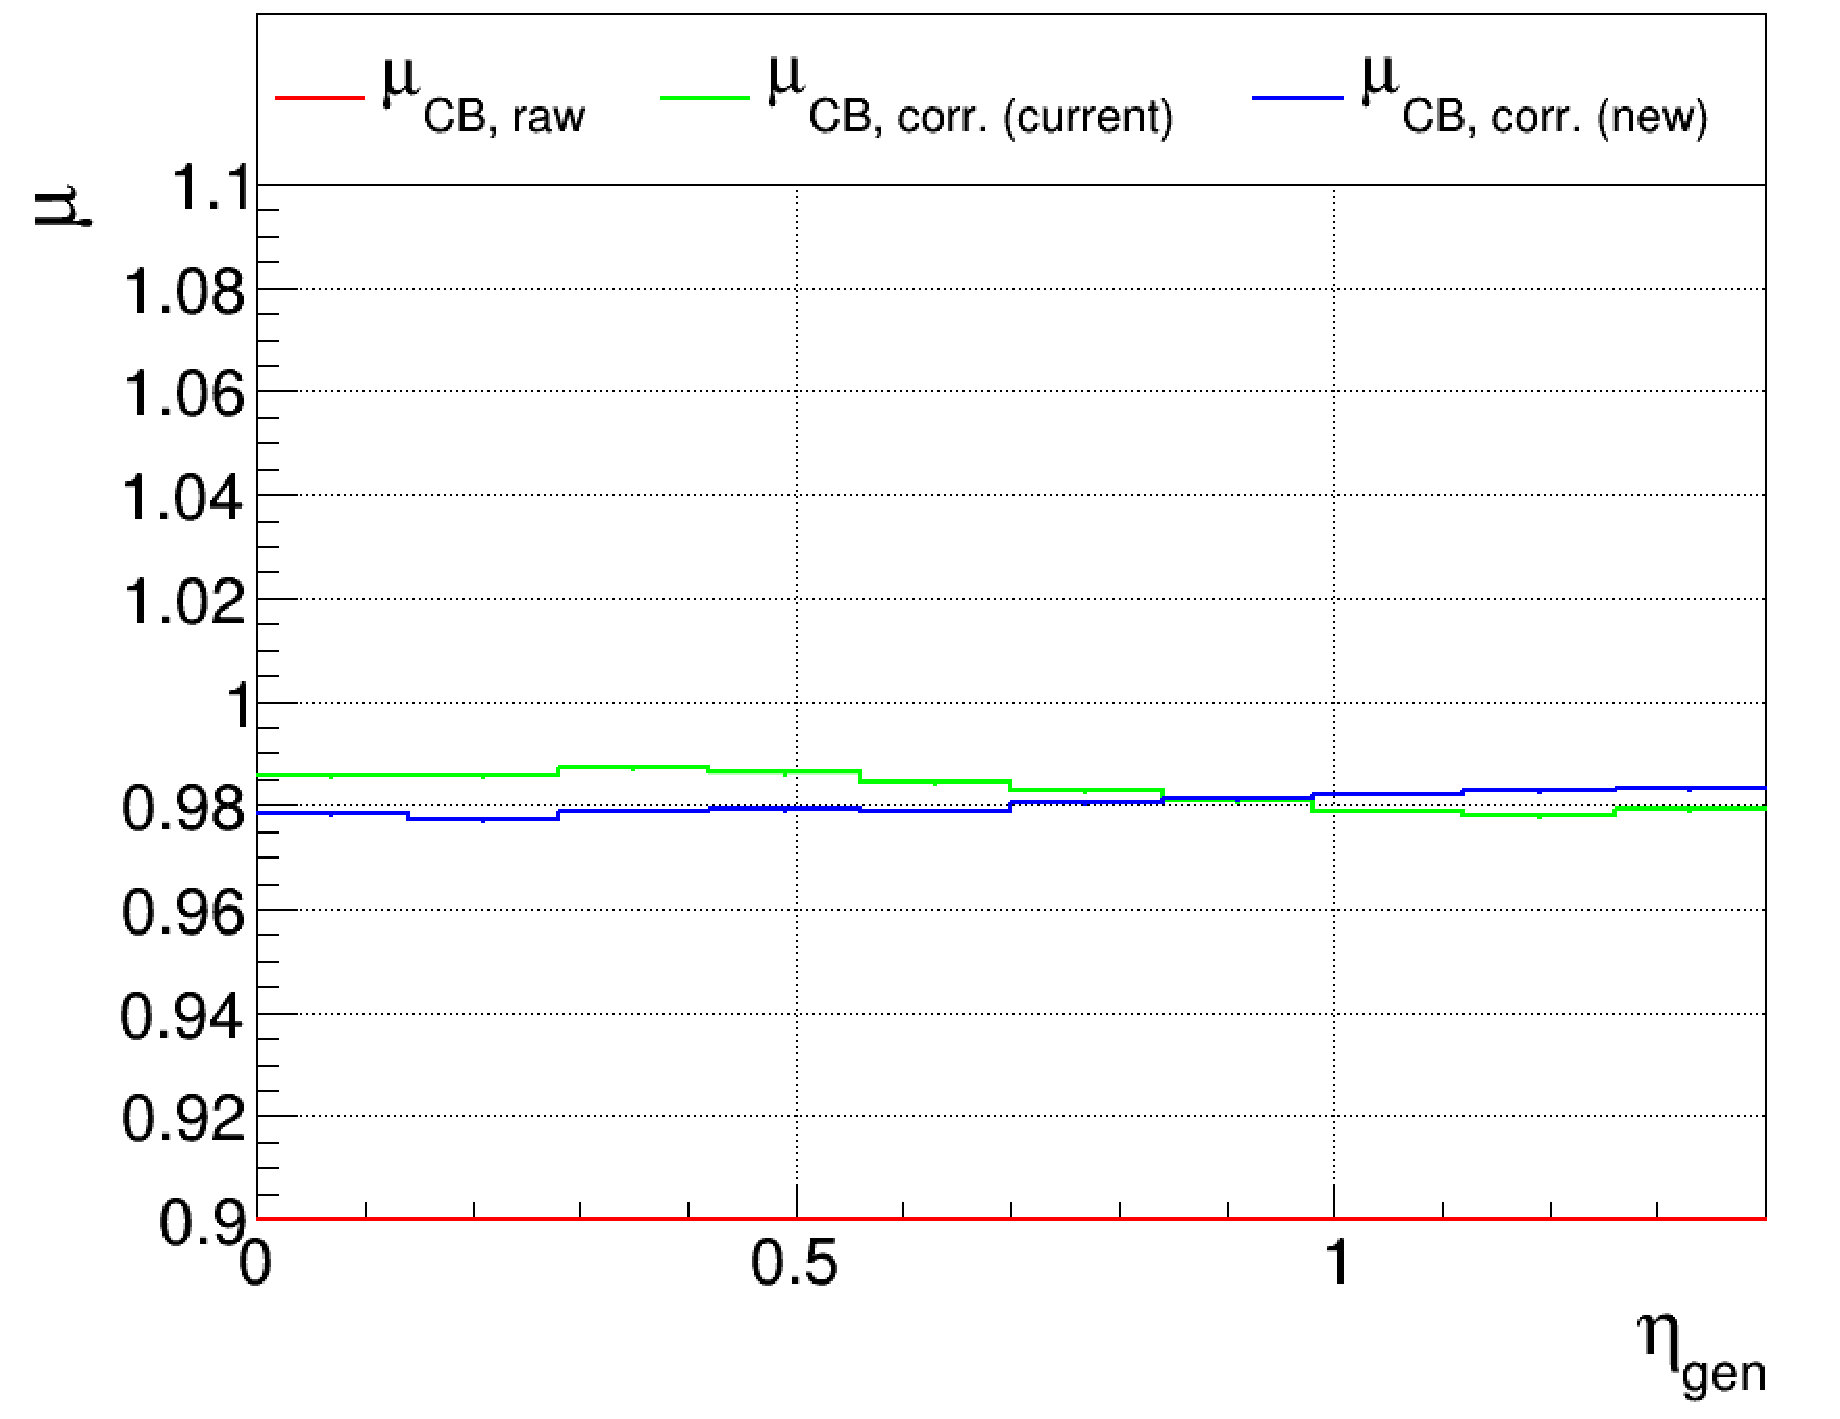
\includegraphics[width=0.495\textwidth]{./plots_pdf/ECAL_plots/plotsPU/EB/FULL/pdf/GENETA/EBFULL_GENETA_0005_0020_MuOverBins.pdf}
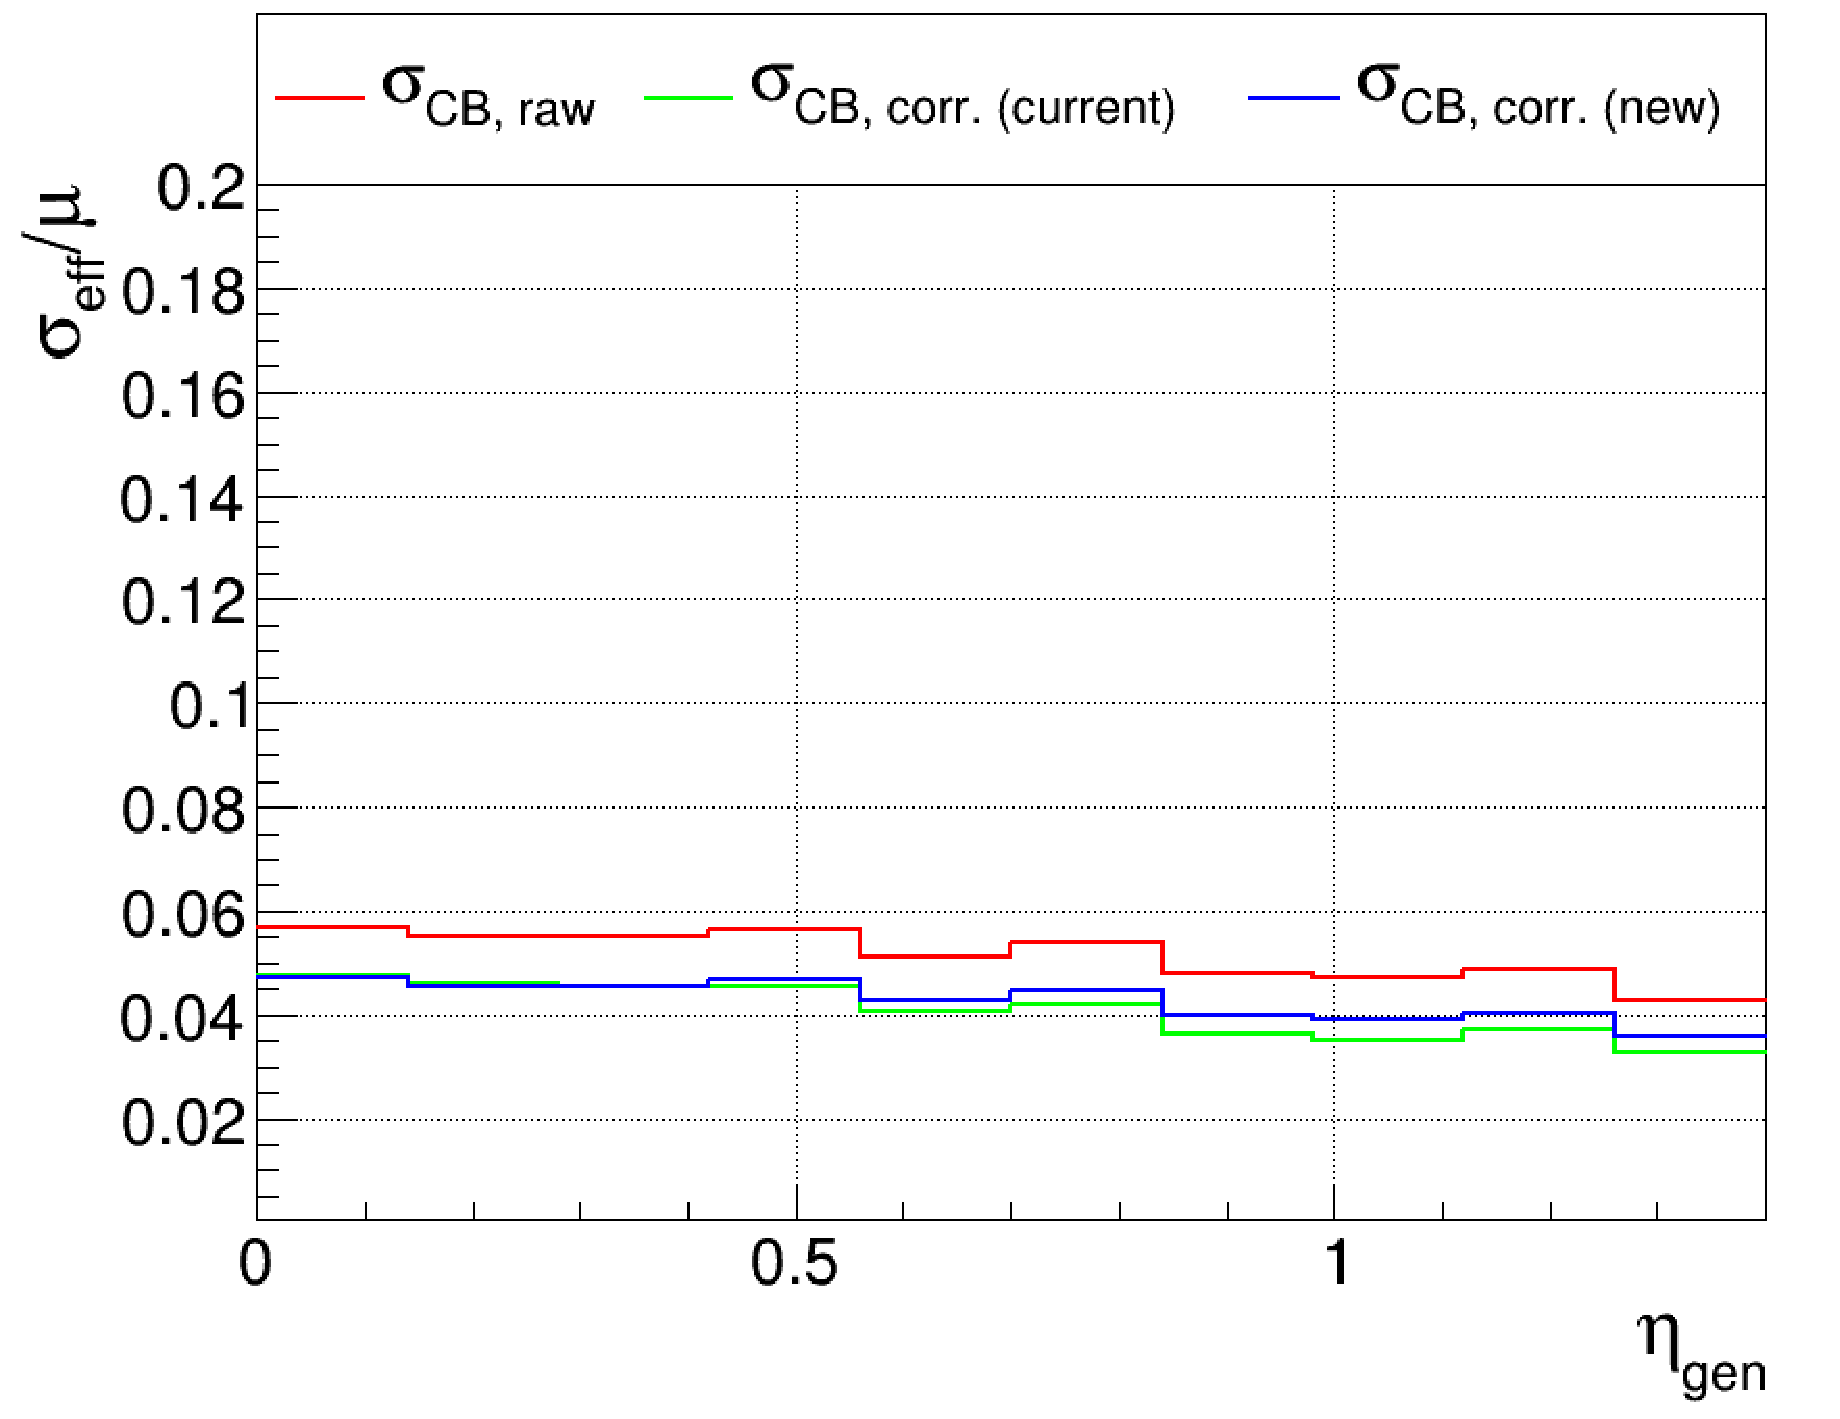
\includegraphics[width=0.495\textwidth]{./plots_pdf/ECAL_plots/plotsPU/EB/FULL/pdf/GENETA/EBFULL_GENETA_0005_0020_EffSigmaOverBins.pdf}
\caption{EB - Full Readout \pt 5--20\GeV.}
\end{figure}


\begin{figure}
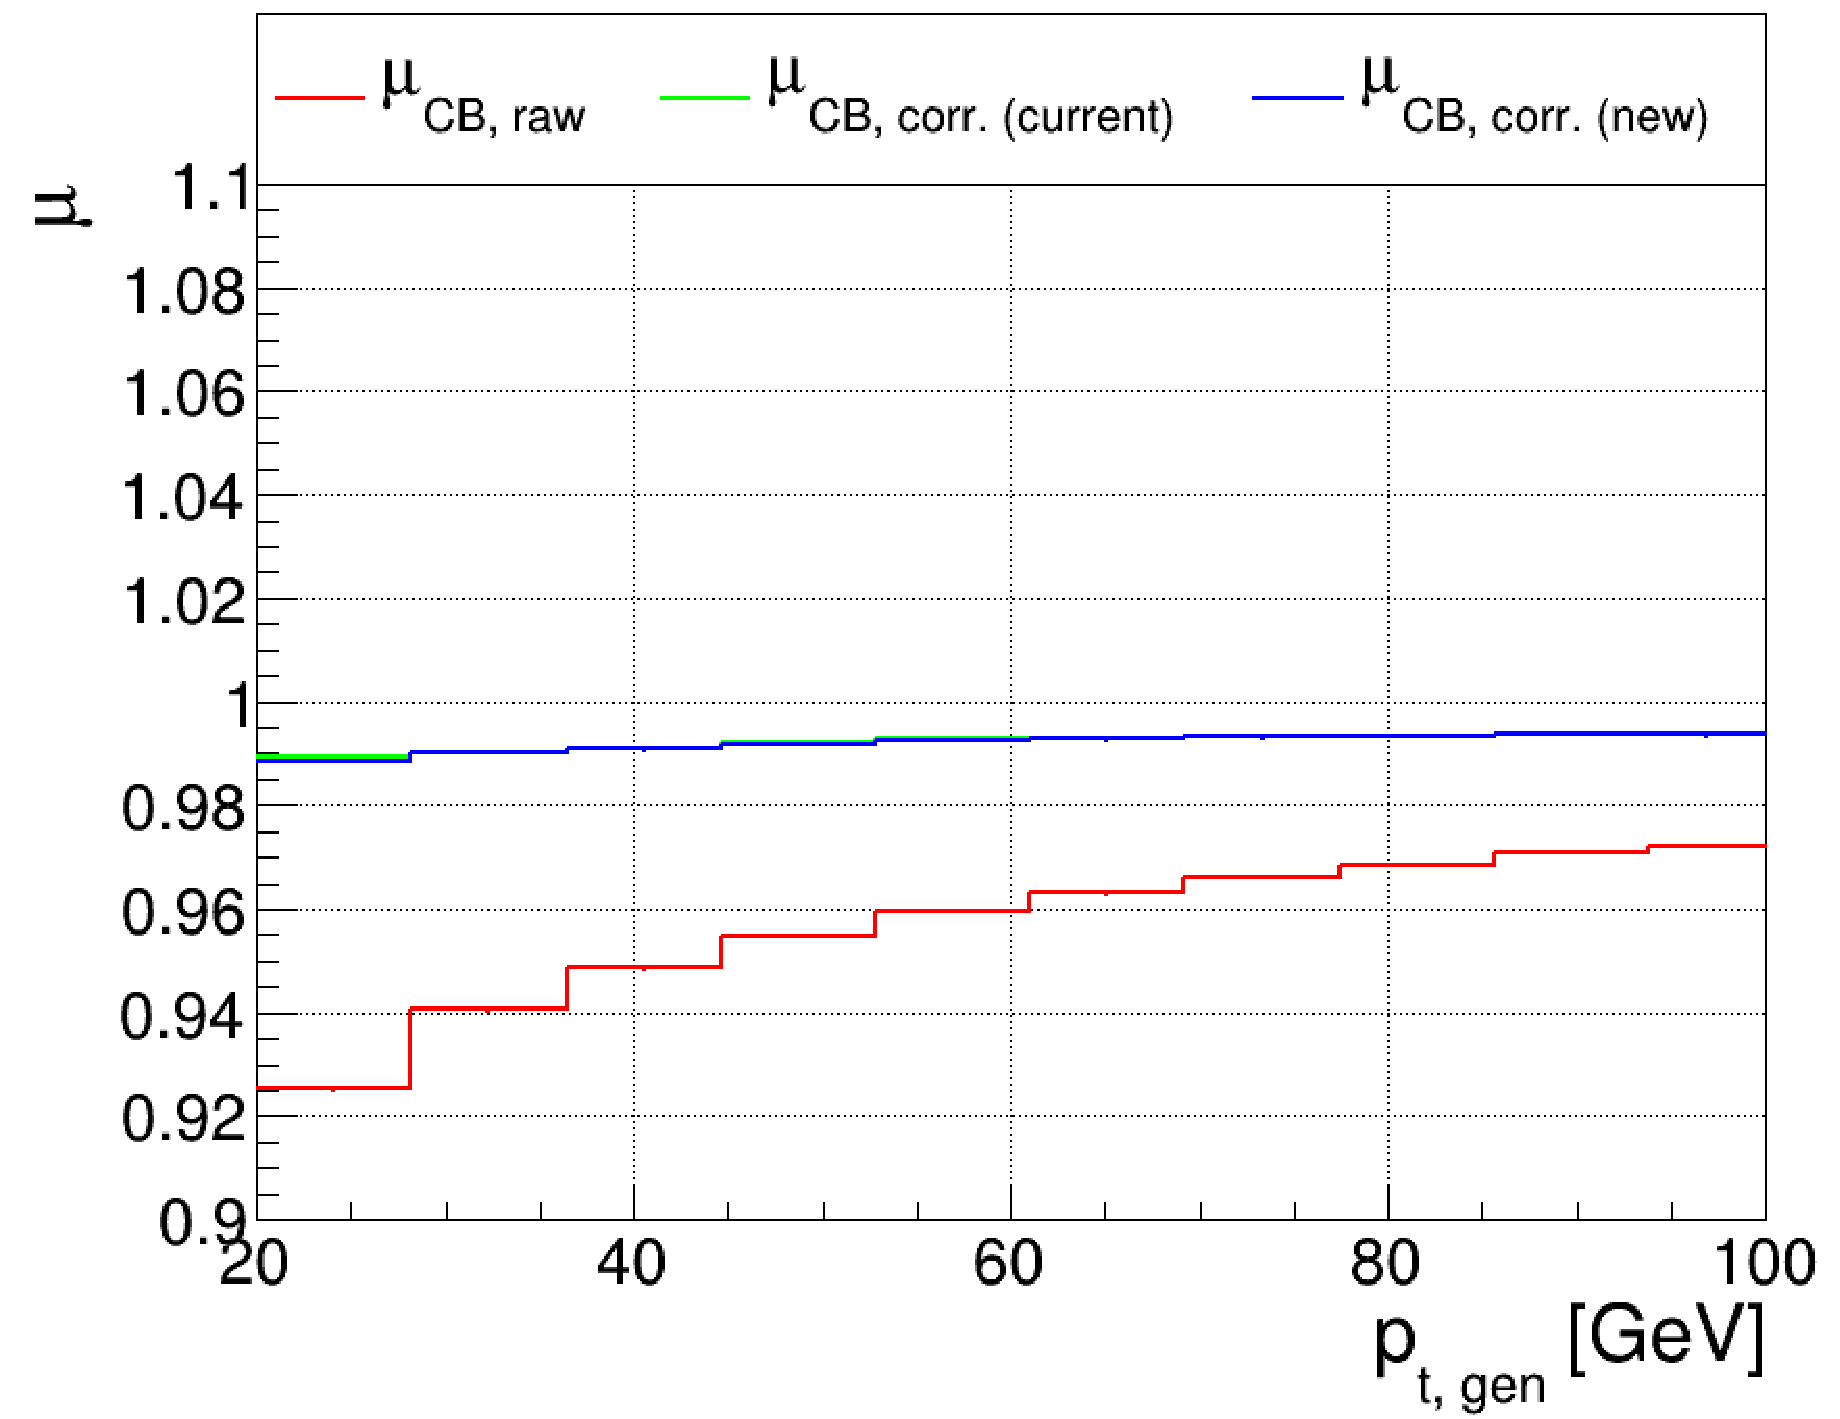
\includegraphics[width=0.495\textwidth]{./plots_pdf/ECAL_plots/plotsPU/EB/FULL/pdf/GENPT/EBFULL_GENPT_0020_0100_MuOverBins.pdf}
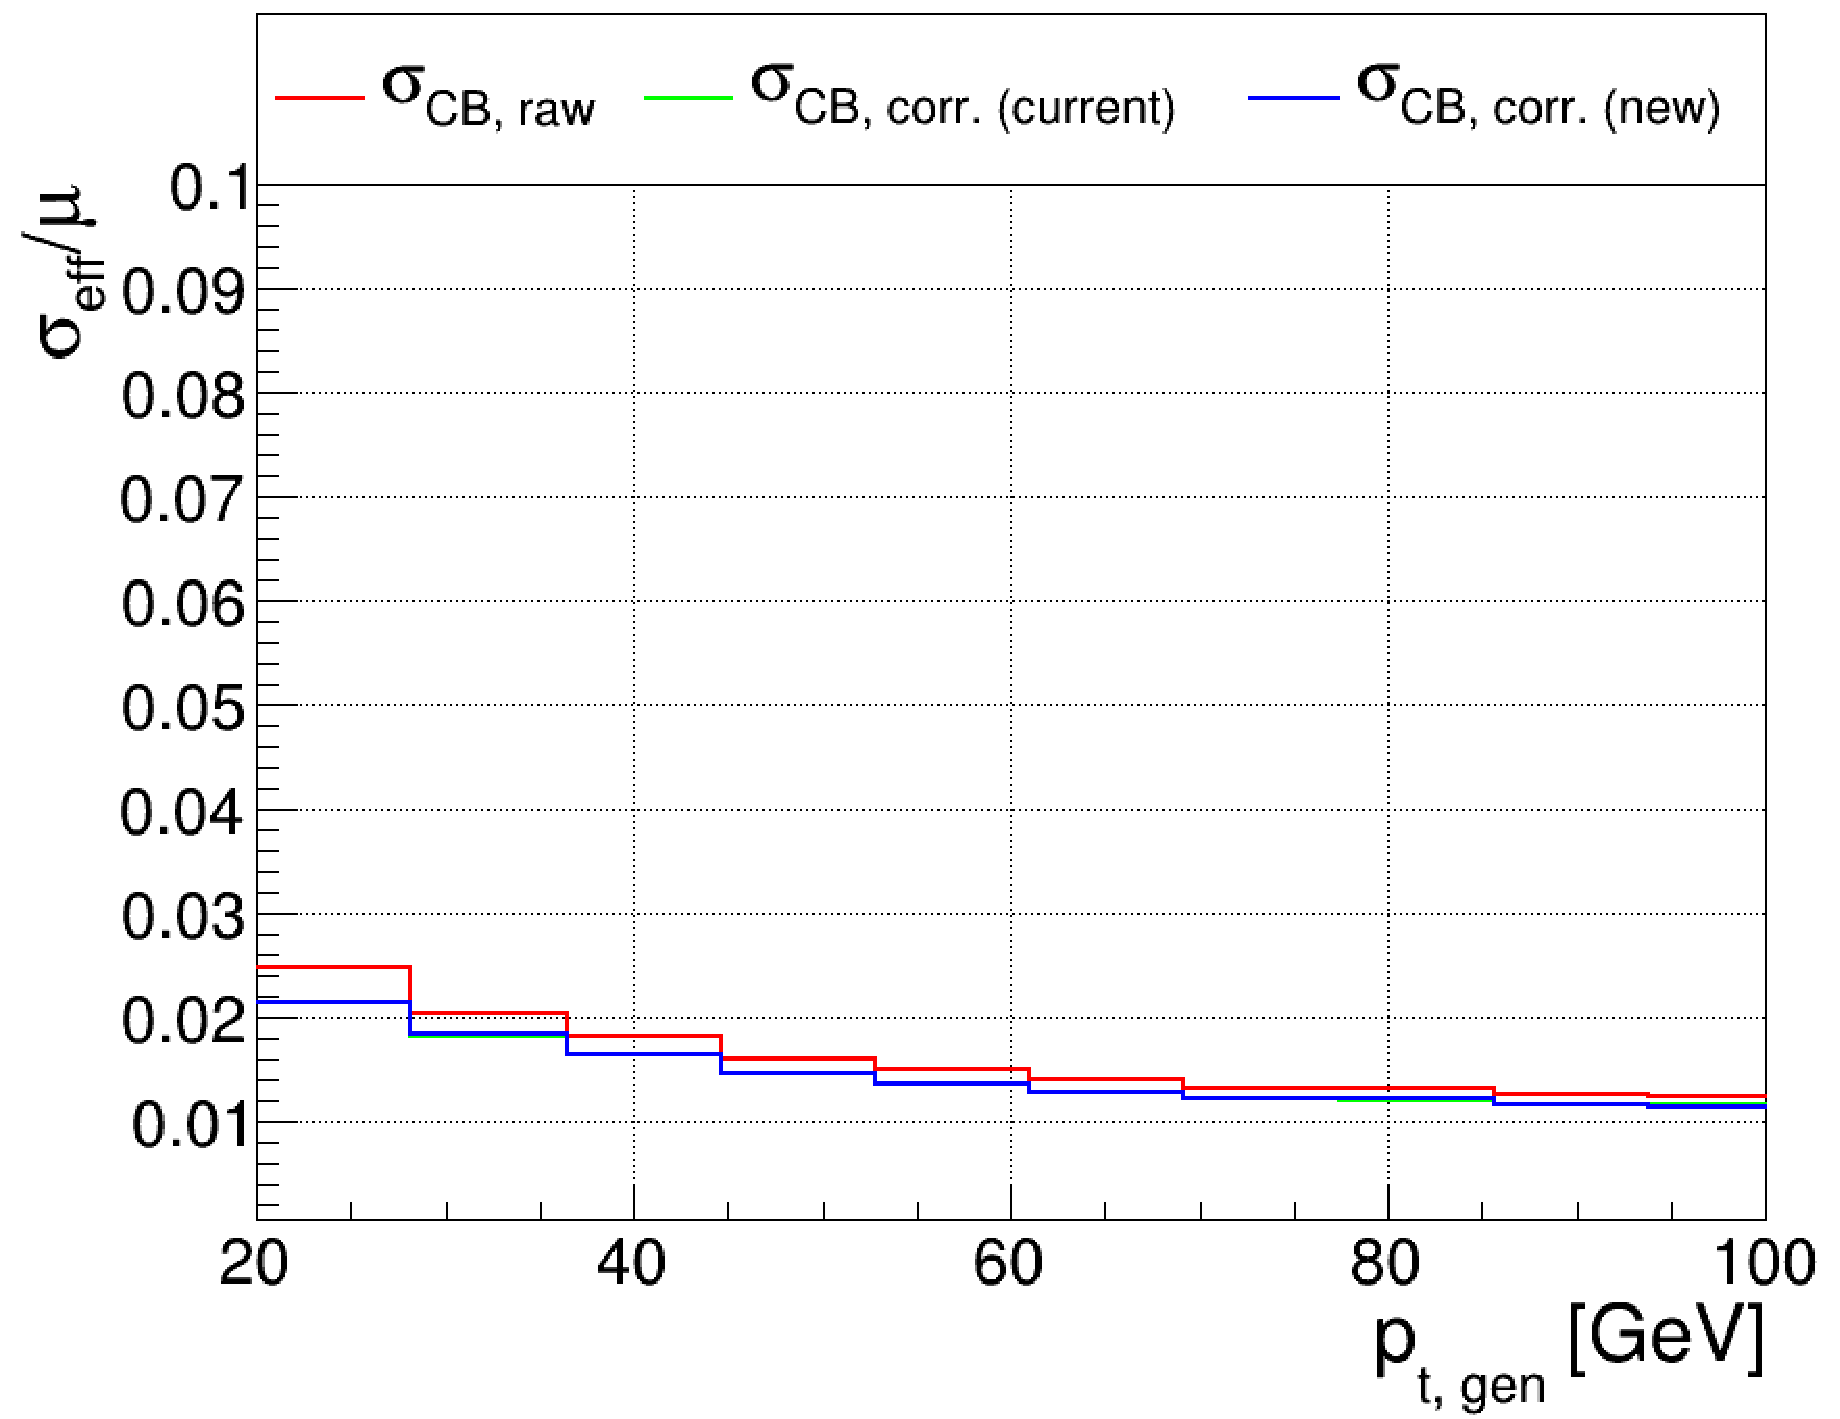
\includegraphics[width=0.495\textwidth]{./plots_pdf/ECAL_plots/plotsPU/EB/FULL/pdf/GENPT/EBFULL_GENPT_0020_0100_EffSigmaOverBins.pdf}
%\caption{EB - Full Readout pt 20-100}
%\end{figure}
%\begin{figure}
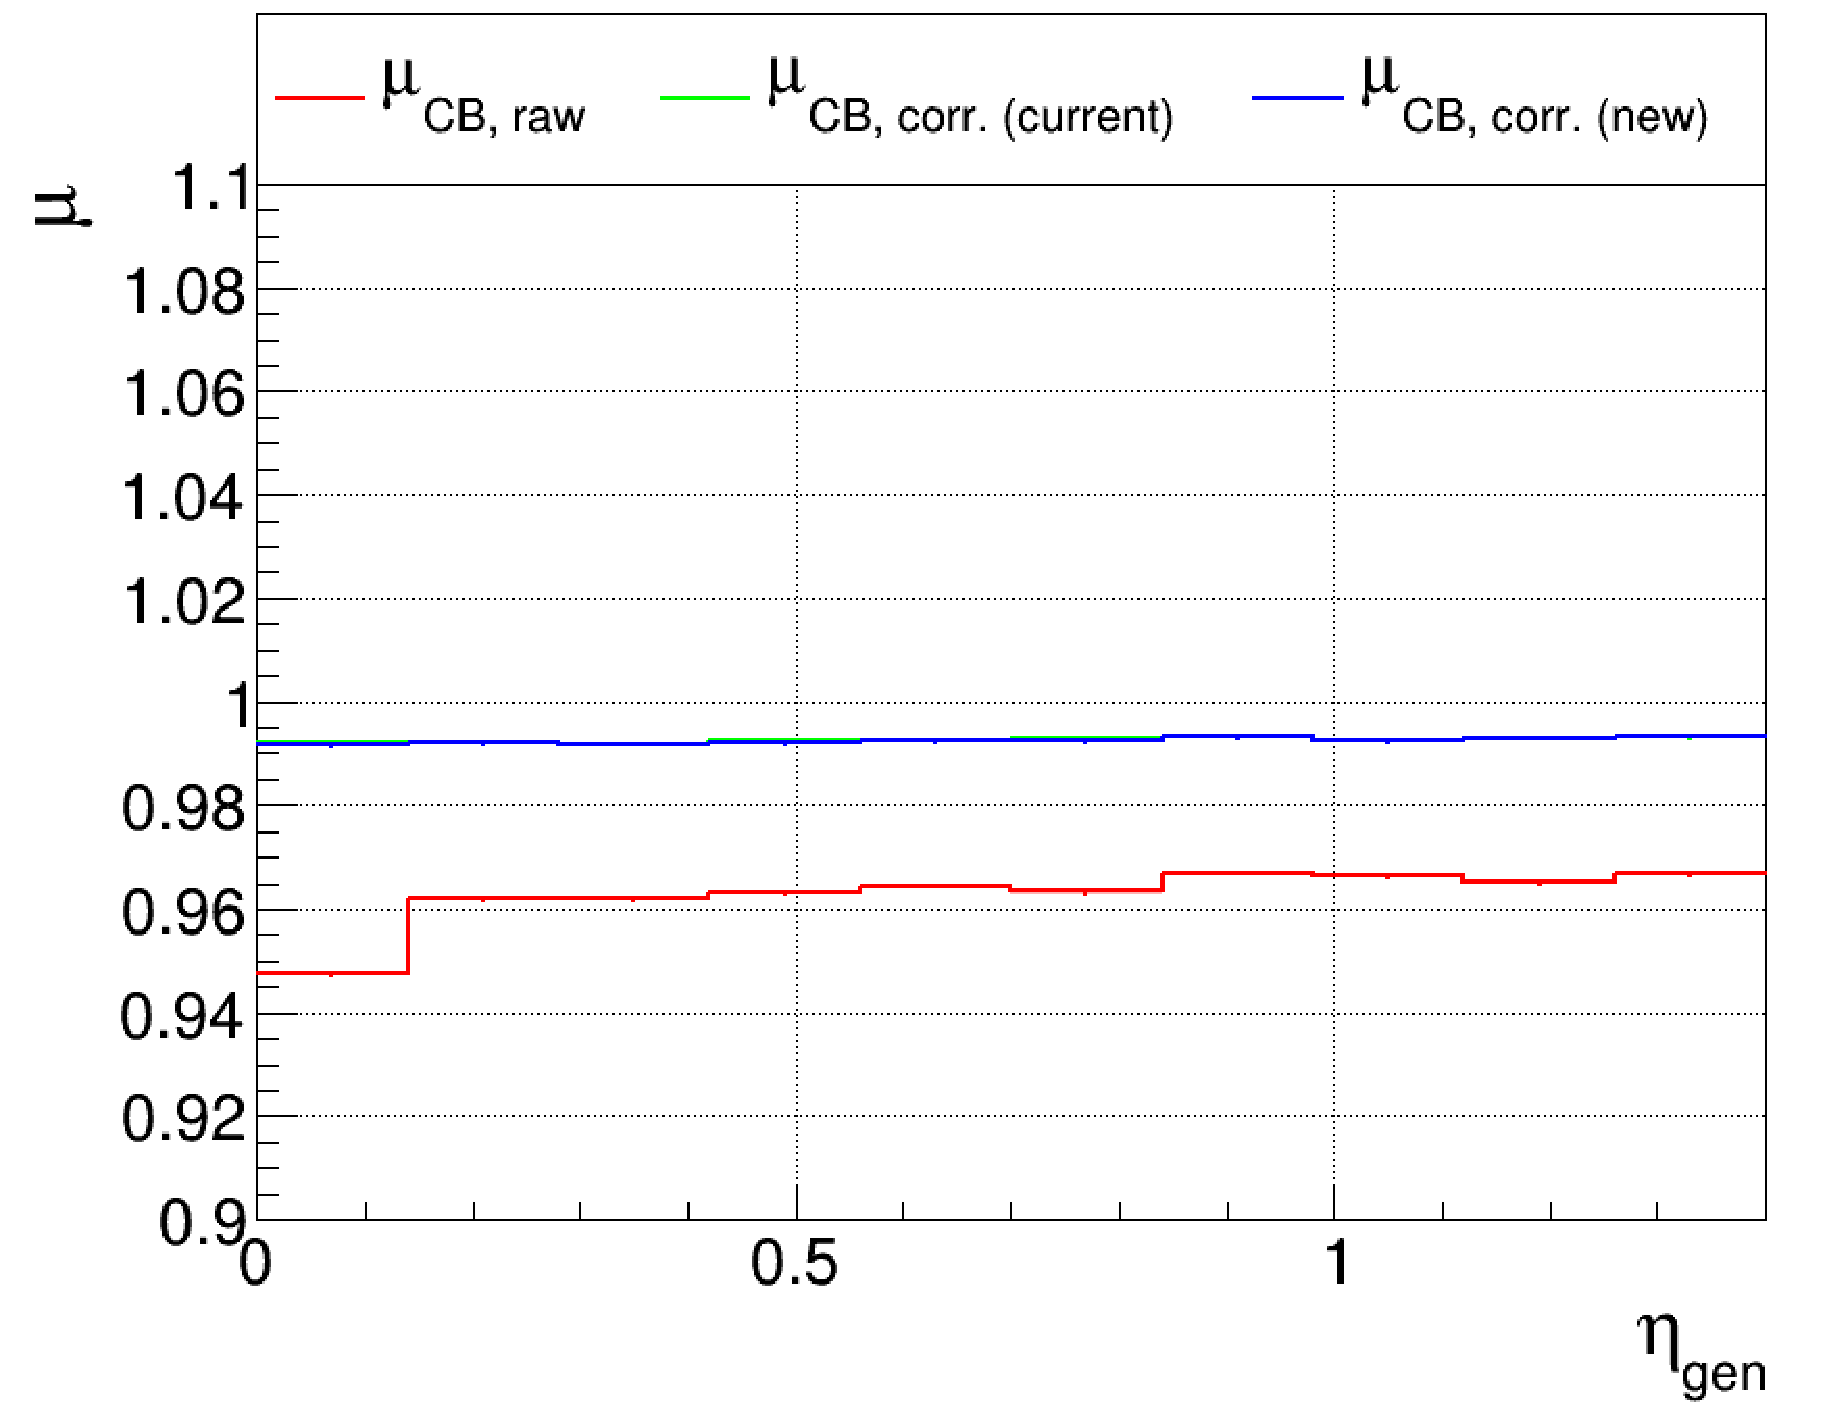
\includegraphics[width=0.495\textwidth]{./plots_pdf/ECAL_plots/plotsPU/EB/FULL/pdf/GENETA/EBFULL_GENETA_0020_0100_MuOverBins.pdf}
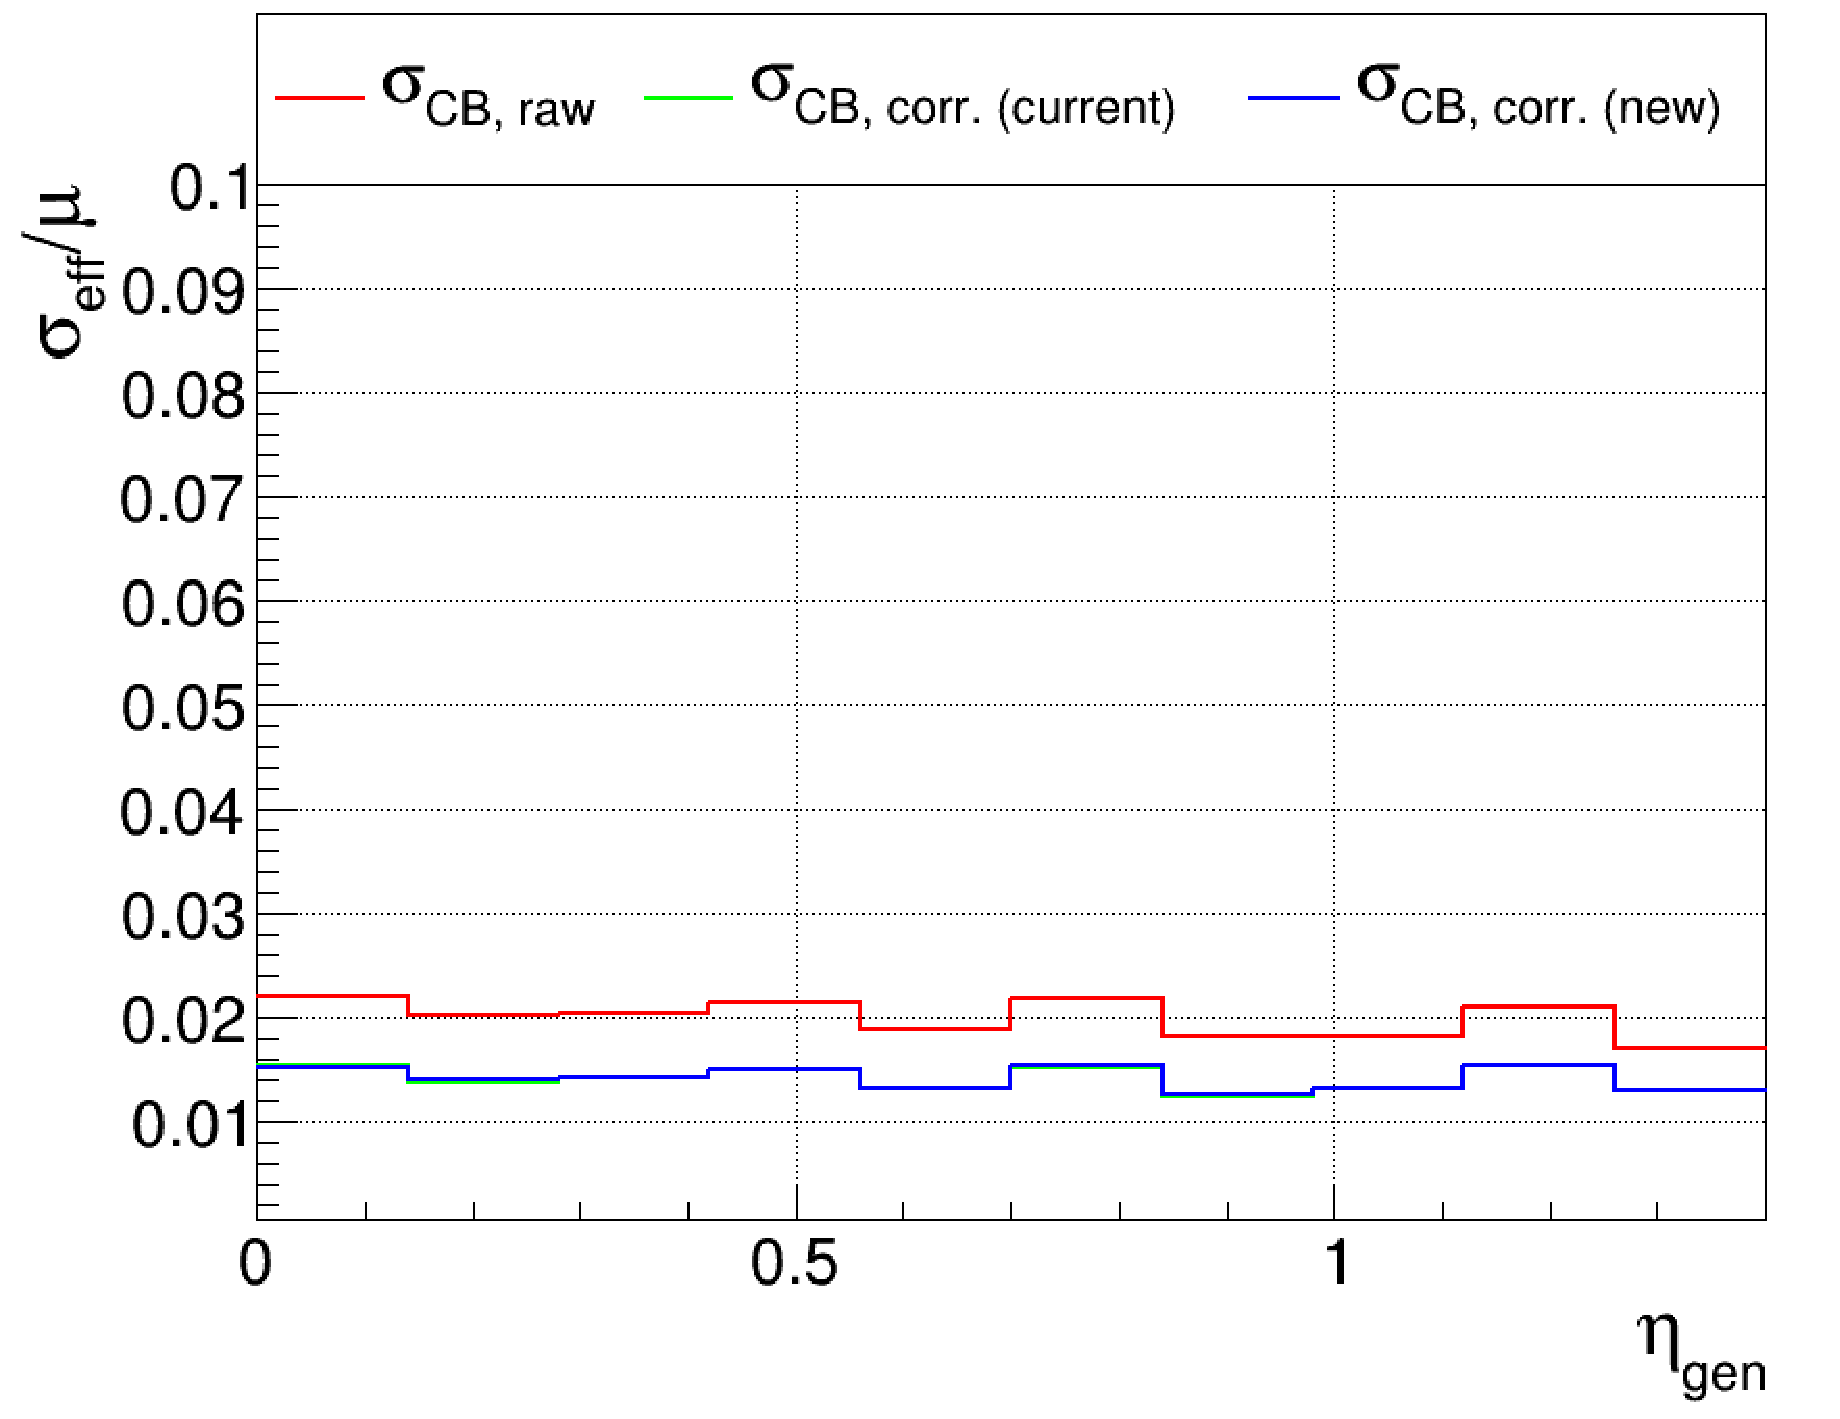
\includegraphics[width=0.495\textwidth]{./plots_pdf/ECAL_plots/plotsPU/EB/FULL/pdf/GENETA/EBFULL_GENETA_0020_0100_EffSigmaOverBins.pdf}
\caption{EB - Full Readout \pt 20--100\GeV.}
\end{figure}

\begin{figure}
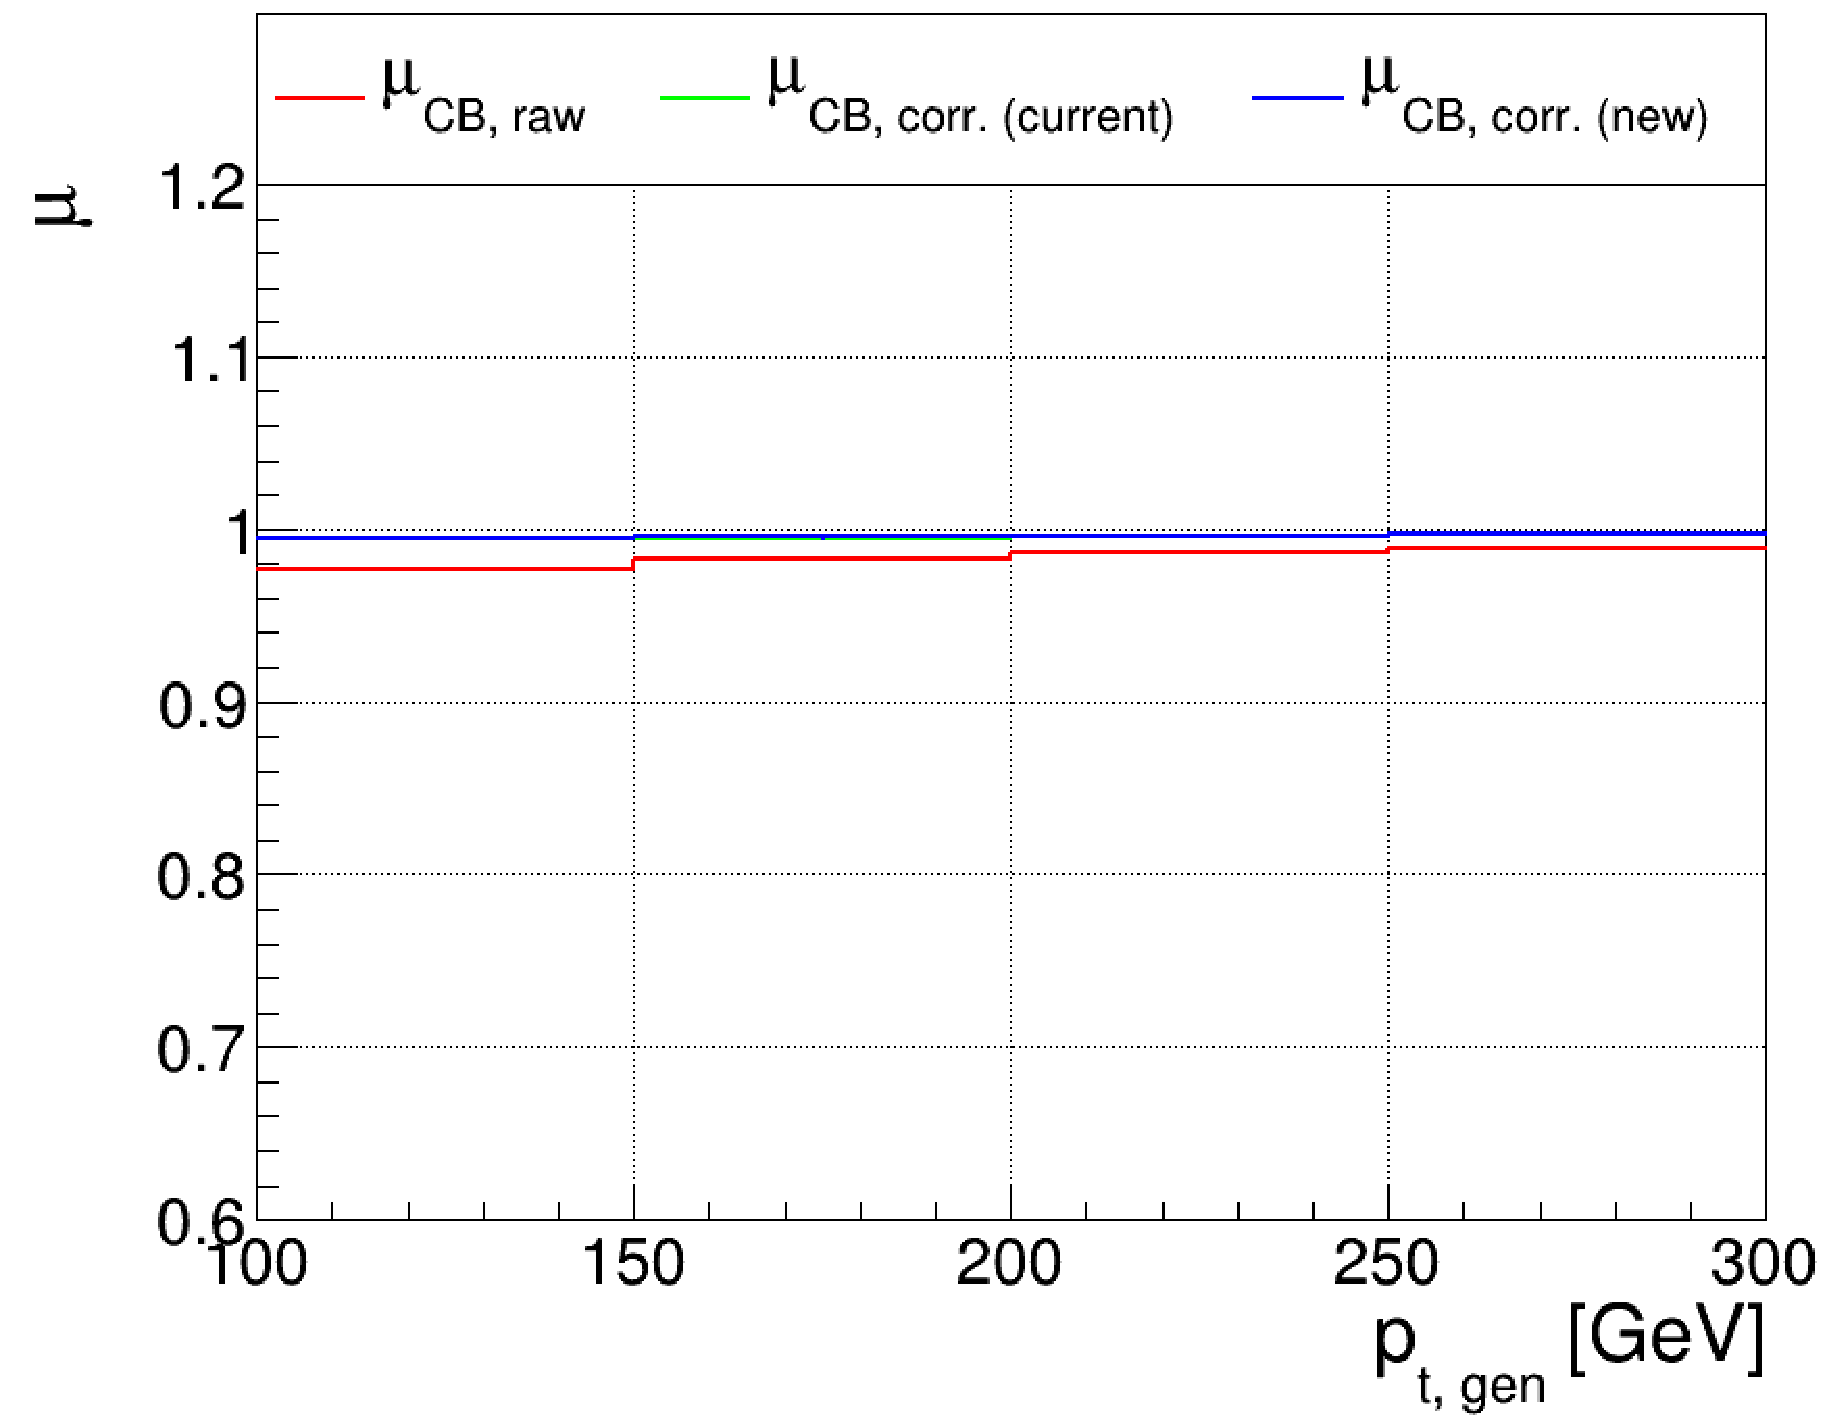
\includegraphics[width=0.495\textwidth]{./plots_pdf/ECAL_plots/plotsPU/EB/FULL/pdf/GENPT/EBFULL_GENPT_0100_0300_MuOverBins.pdf}
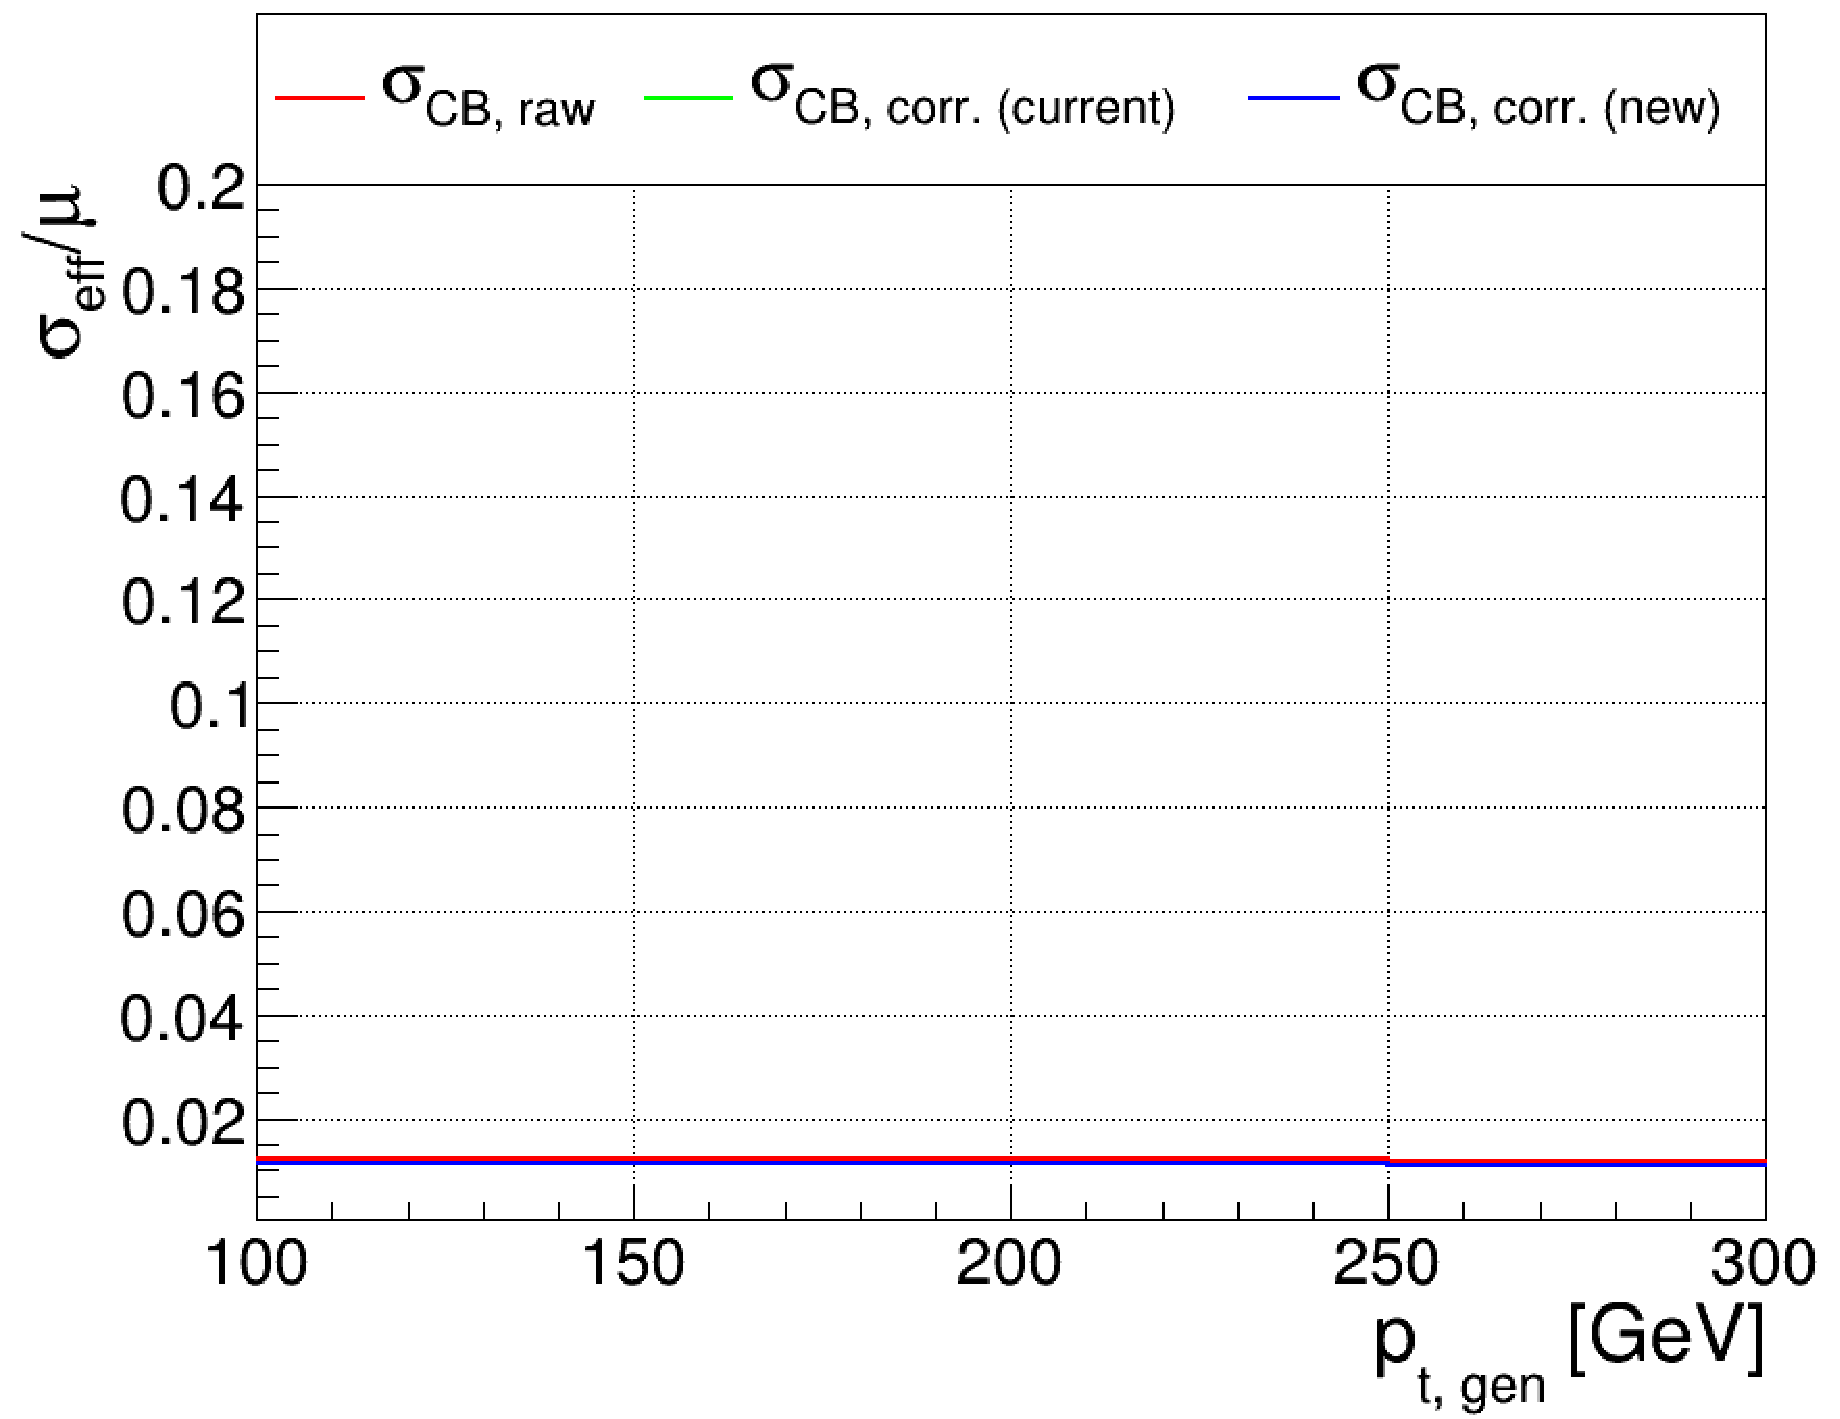
\includegraphics[width=0.495\textwidth]{./plots_pdf/ECAL_plots/plotsPU/EB/FULL/pdf/GENPT/EBFULL_GENPT_0100_0300_EffSigmaOverBins.pdf}
%\caption{EB - Full Readout pt 100-300}
%\end{figure}
%\begin{figure}
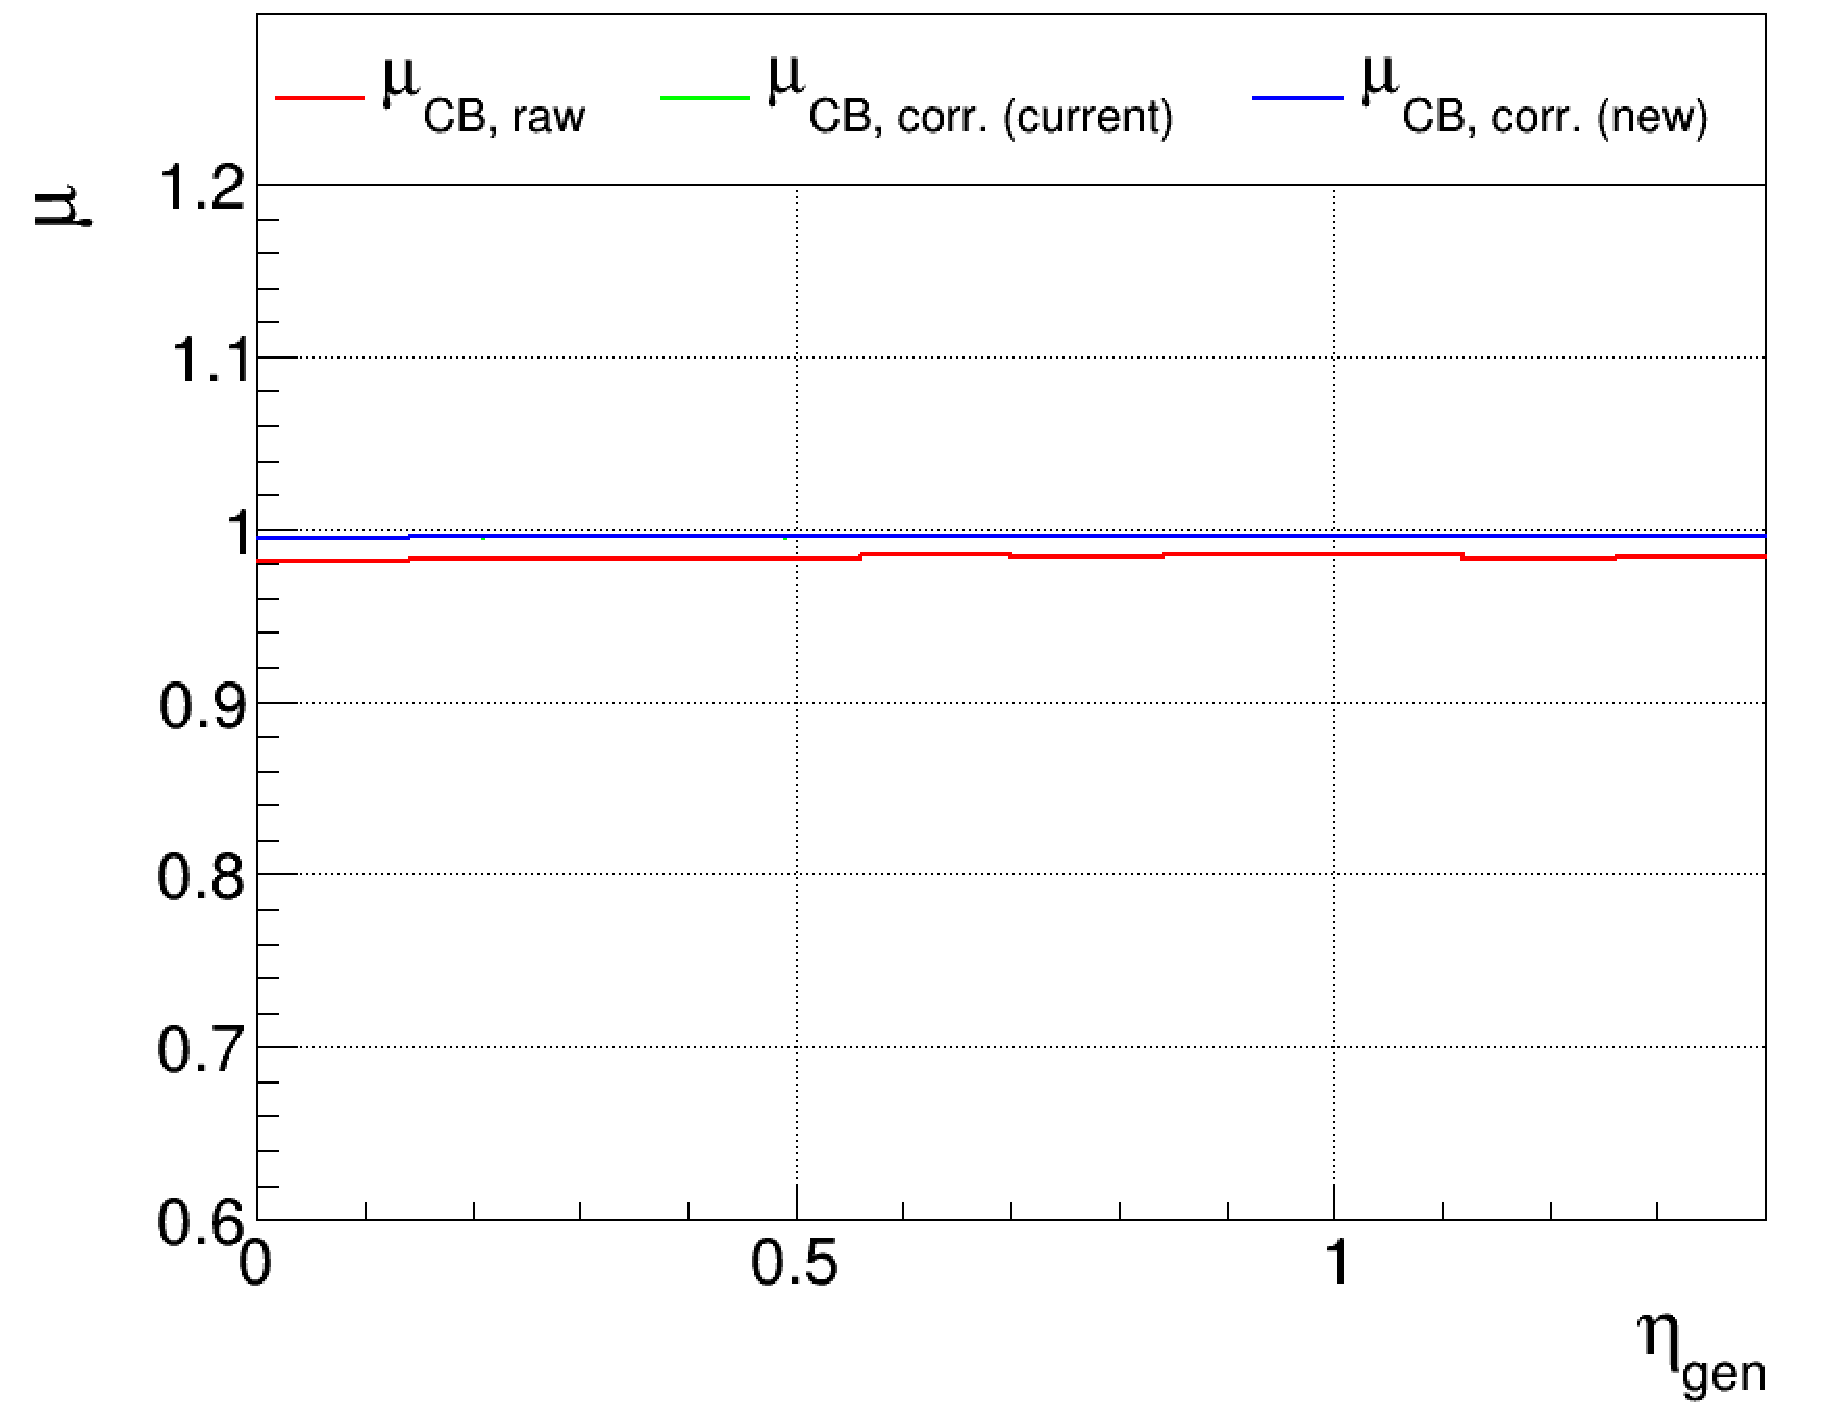
\includegraphics[width=0.495\textwidth]{./plots_pdf/ECAL_plots/plotsPU/EB/FULL/pdf/GENETA/EBFULL_GENETA_0100_0300_MuOverBins.pdf}
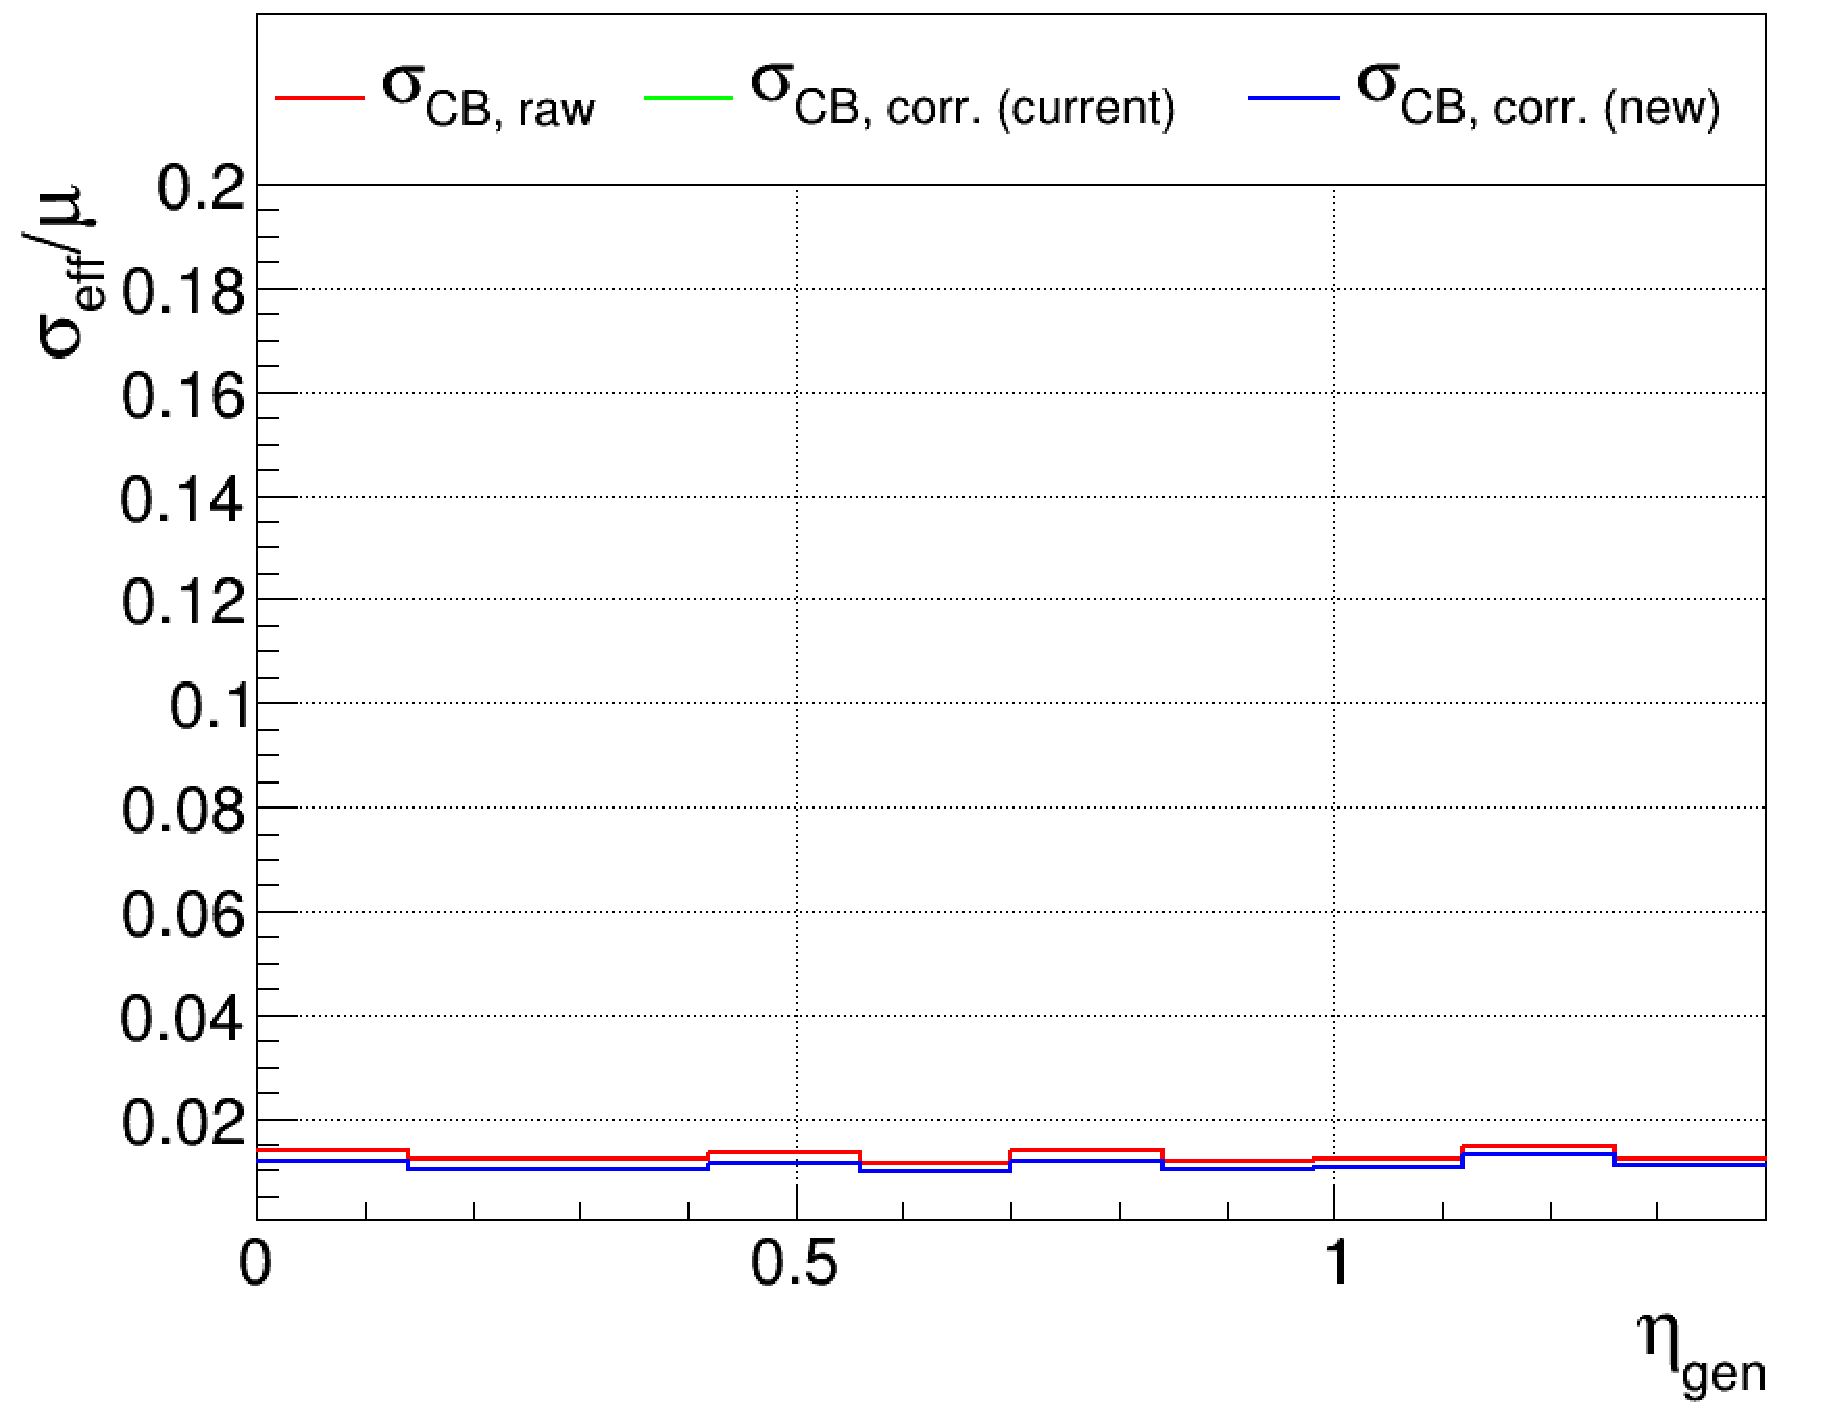
\includegraphics[width=0.495\textwidth]{./plots_pdf/ECAL_plots/plotsPU/EB/FULL/pdf/GENETA/EBFULL_GENETA_0100_0300_EffSigmaOverBins.pdf}
\caption{EB - Full Readout \pt 100-300\GeV}
\end{figure}





\begin{figure}
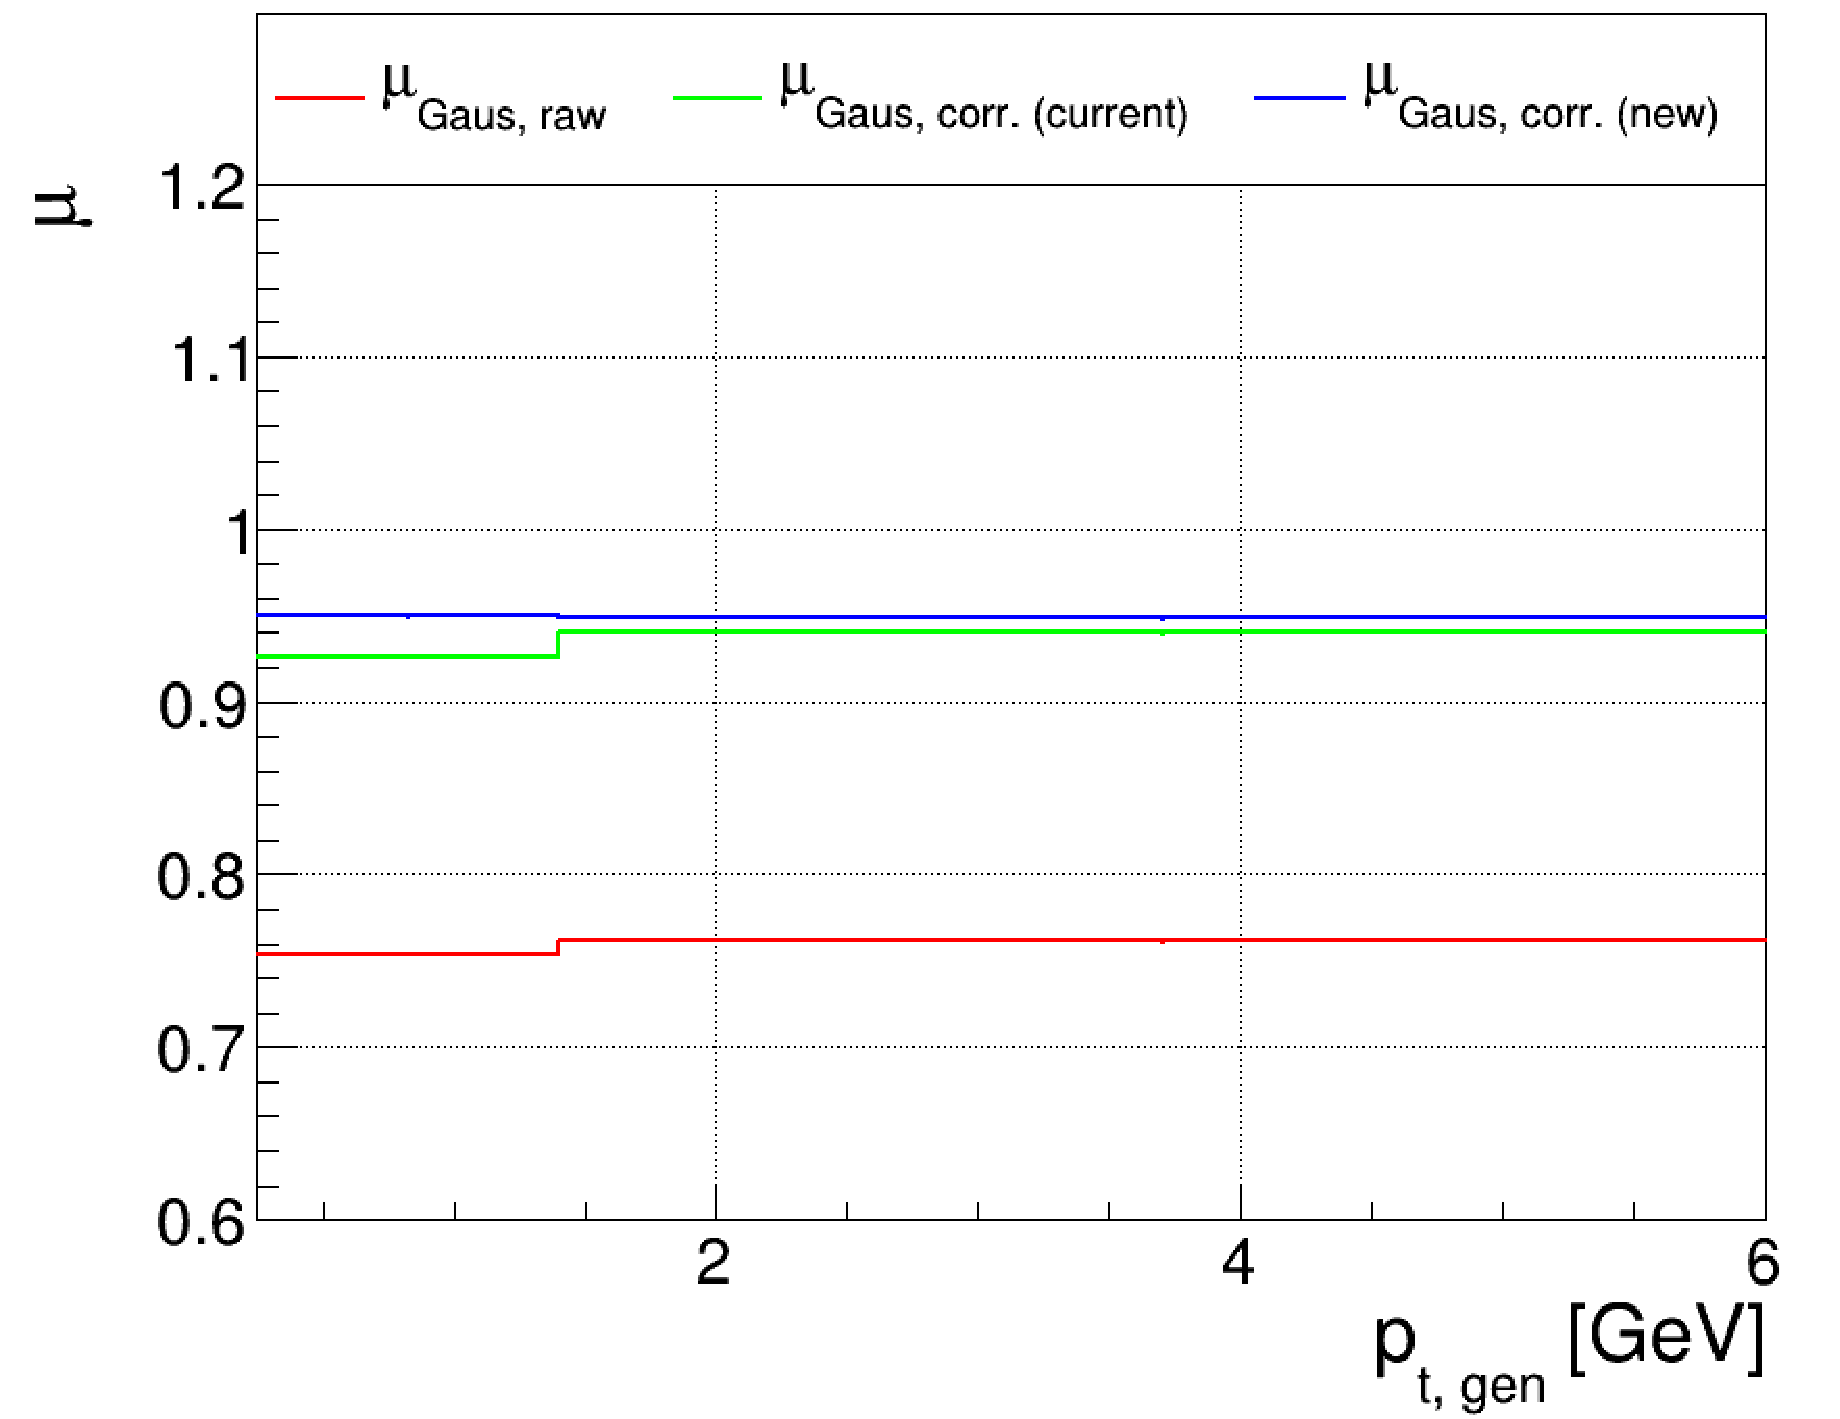
\includegraphics[width=0.495\textwidth]{./plots_pdf/ECAL_plots/plotsPU/EB/ZS/pdf/GENPT/EBZS_GENPT_0000_0006_MuOverBins.pdf}
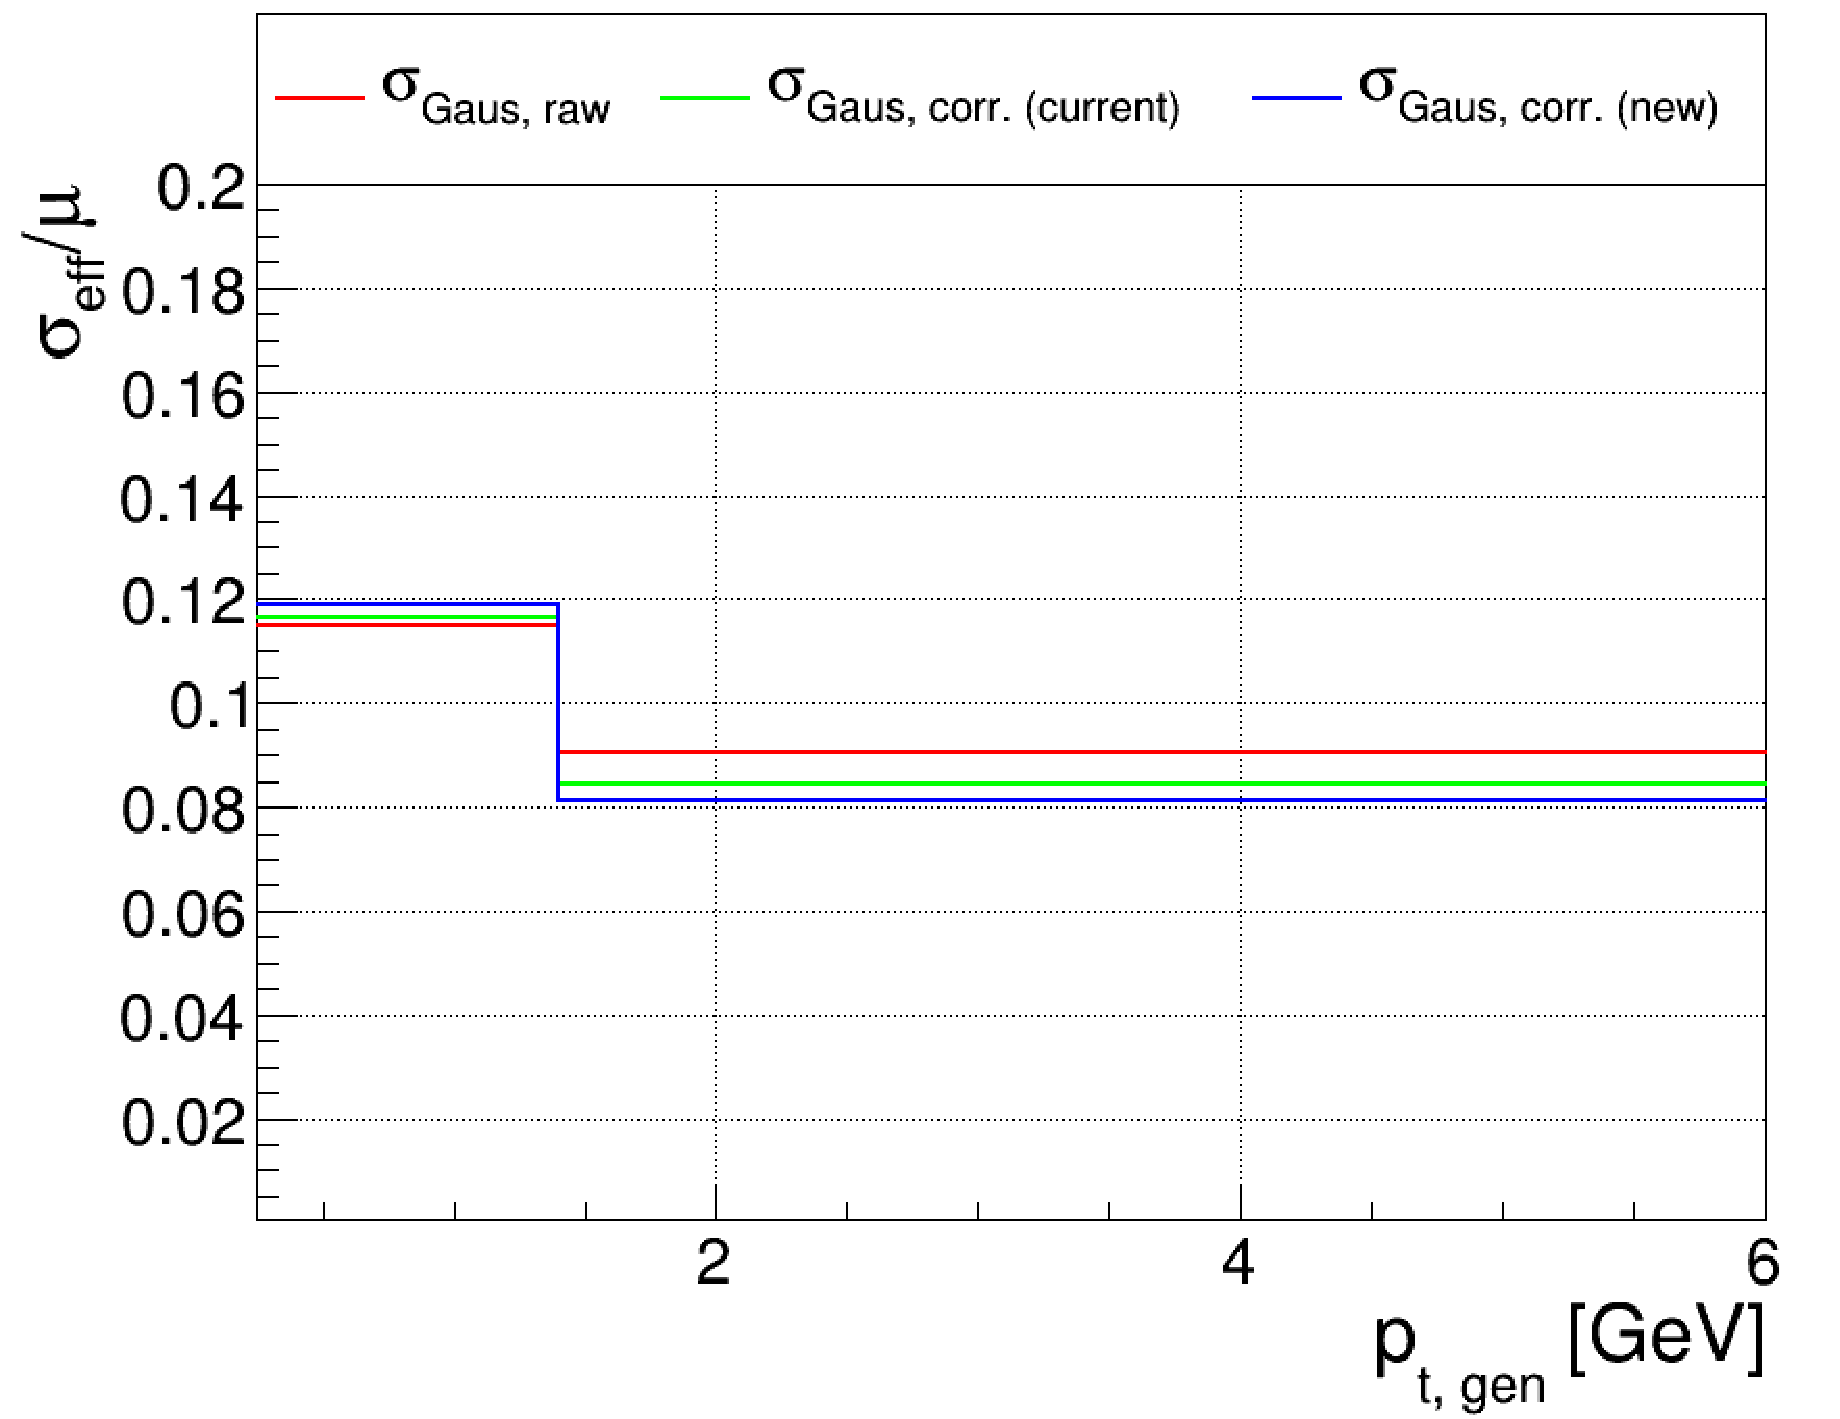
\includegraphics[width=0.495\textwidth]{./plots_pdf/ECAL_plots/plotsPU/EB/ZS/pdf/GENPT/EBZS_GENPT_0000_0006_EffSigmaOverBins.pdf}

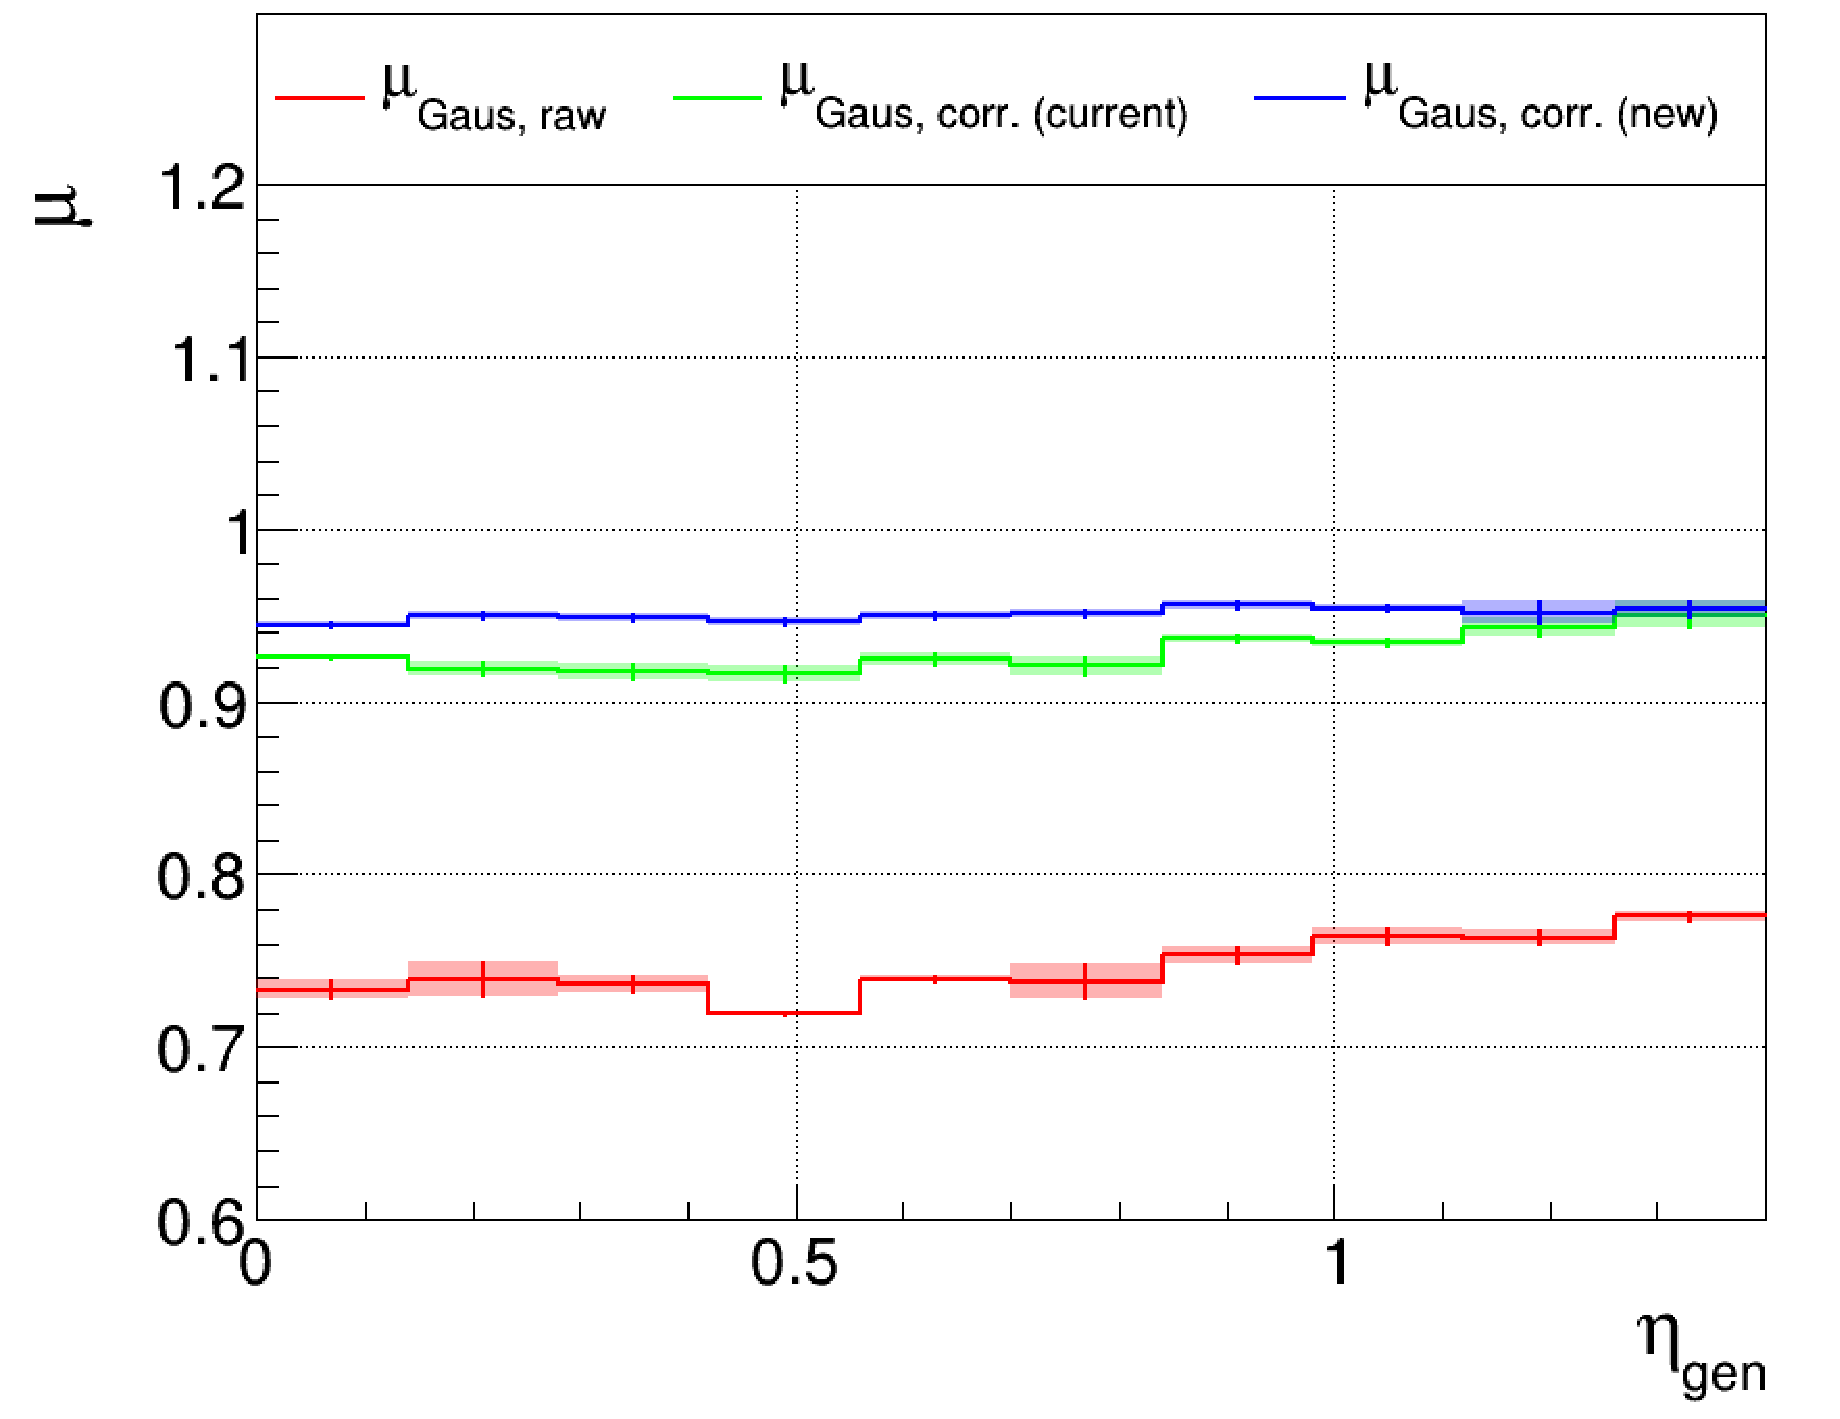
\includegraphics[width=0.495\textwidth]{./plots_pdf/ECAL_plots/plotsPU/EB/ZS/pdf/GENETA/EBZS_GENETA_0000_0006_MuOverBins.pdf}
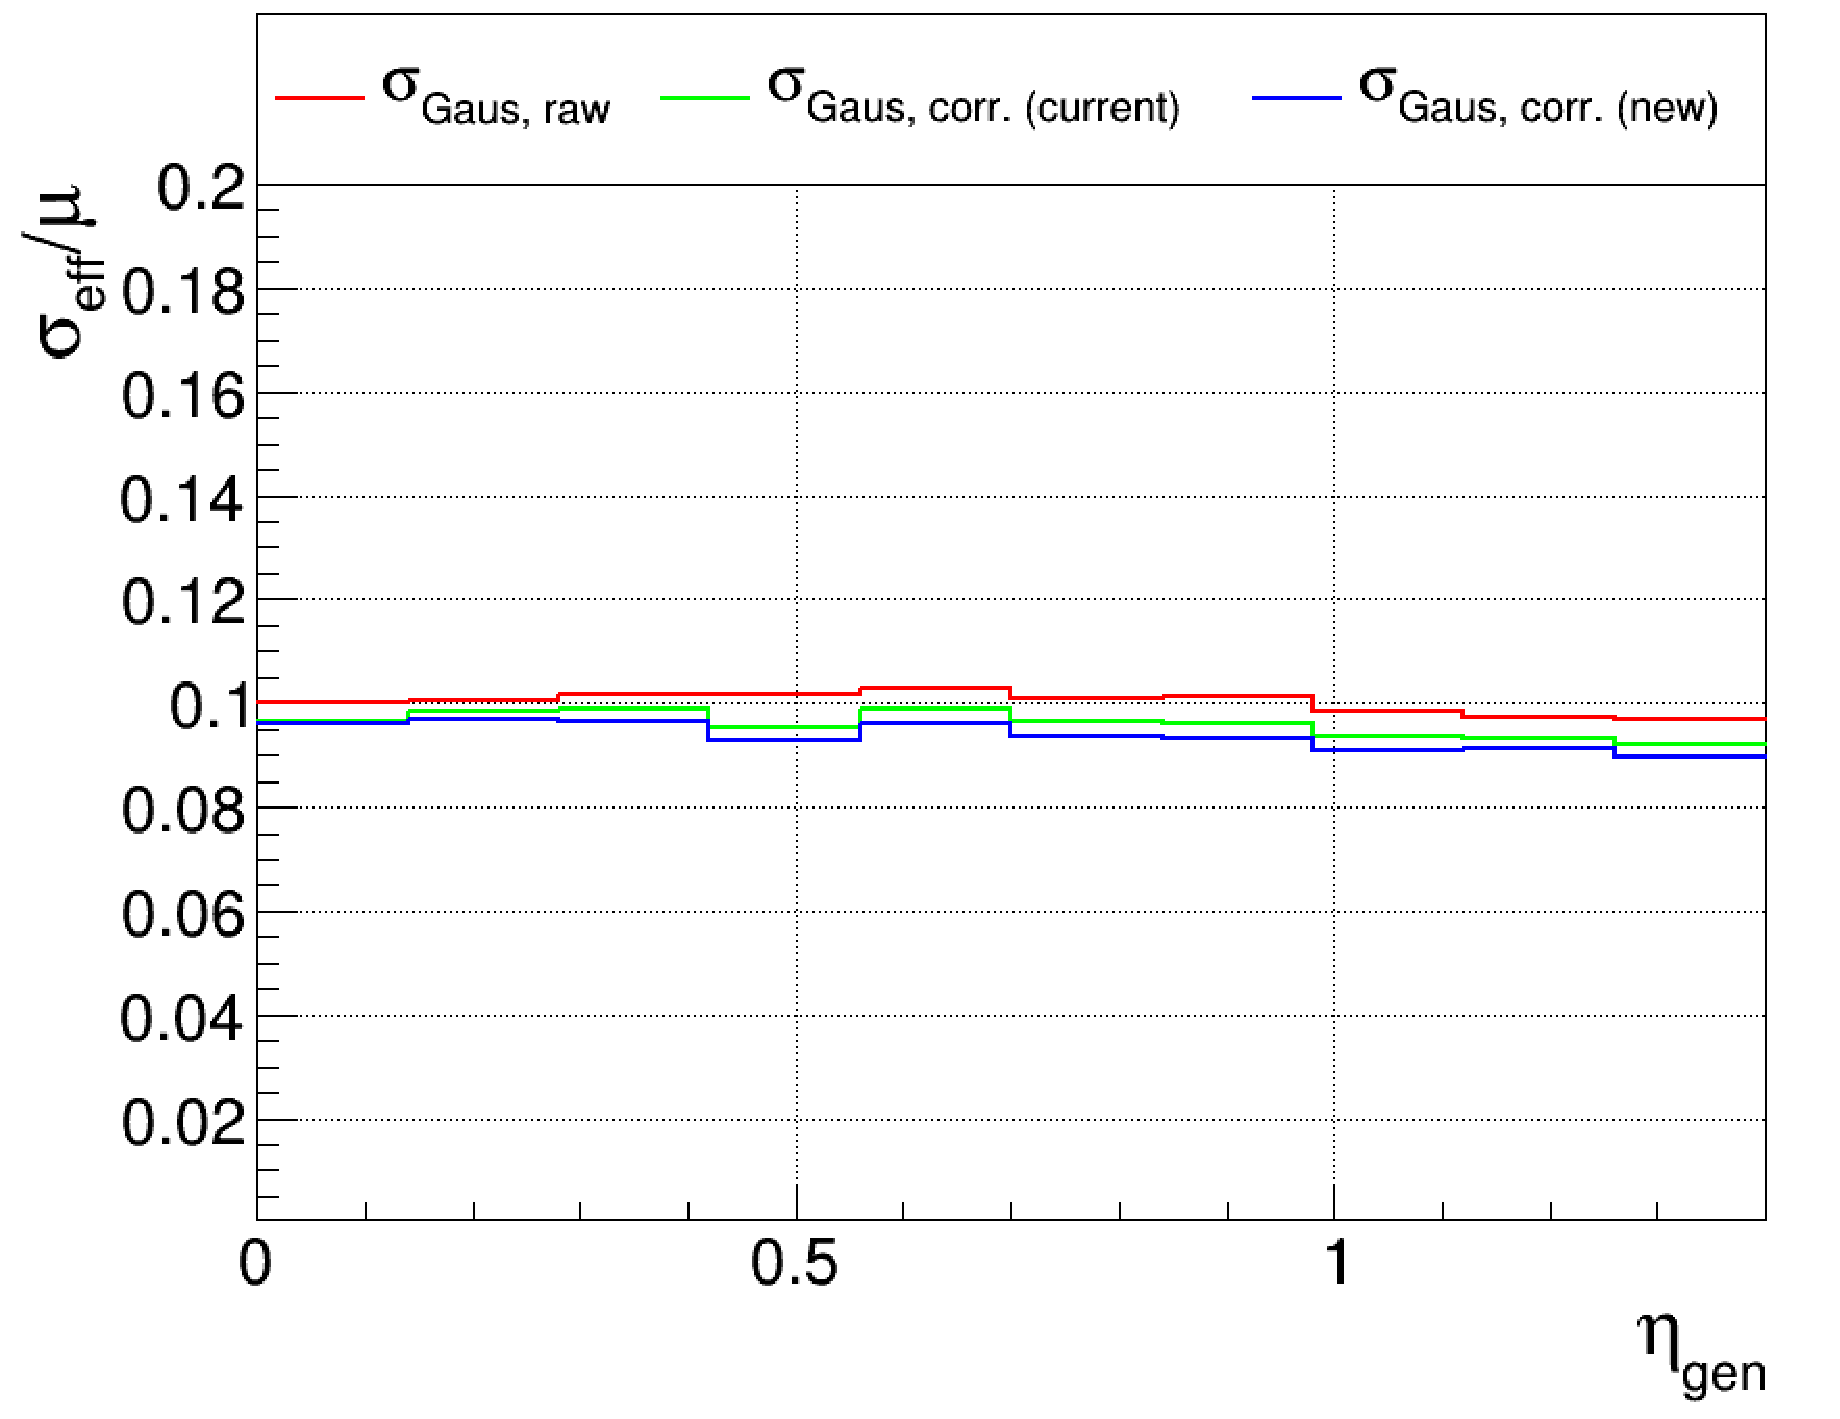
\includegraphics[width=0.495\textwidth]{./plots_pdf/ECAL_plots/plotsPU/EB/ZS/pdf/GENETA/EBZS_GENETA_0000_0006_EffSigmaOverBins.pdf}
\caption[$\mu$ ($\sigma_\mathrm{eff}$) vs \pt of PF ECAL cluster - EB ZS readout PU  senario]{Mean response (resolution) defined by Raw PF ECAL clusters (red), the calibration derived earlier in Ru\
n3 based on 126X (green), and the new correction from 2024 simulation sample based on 133X (blue). \pt 0--6\GeV PU EB ZS readout PU senario.}
\label{fig:PU_EBZS}
\end{figure}

%% %\begin{figure}
%% 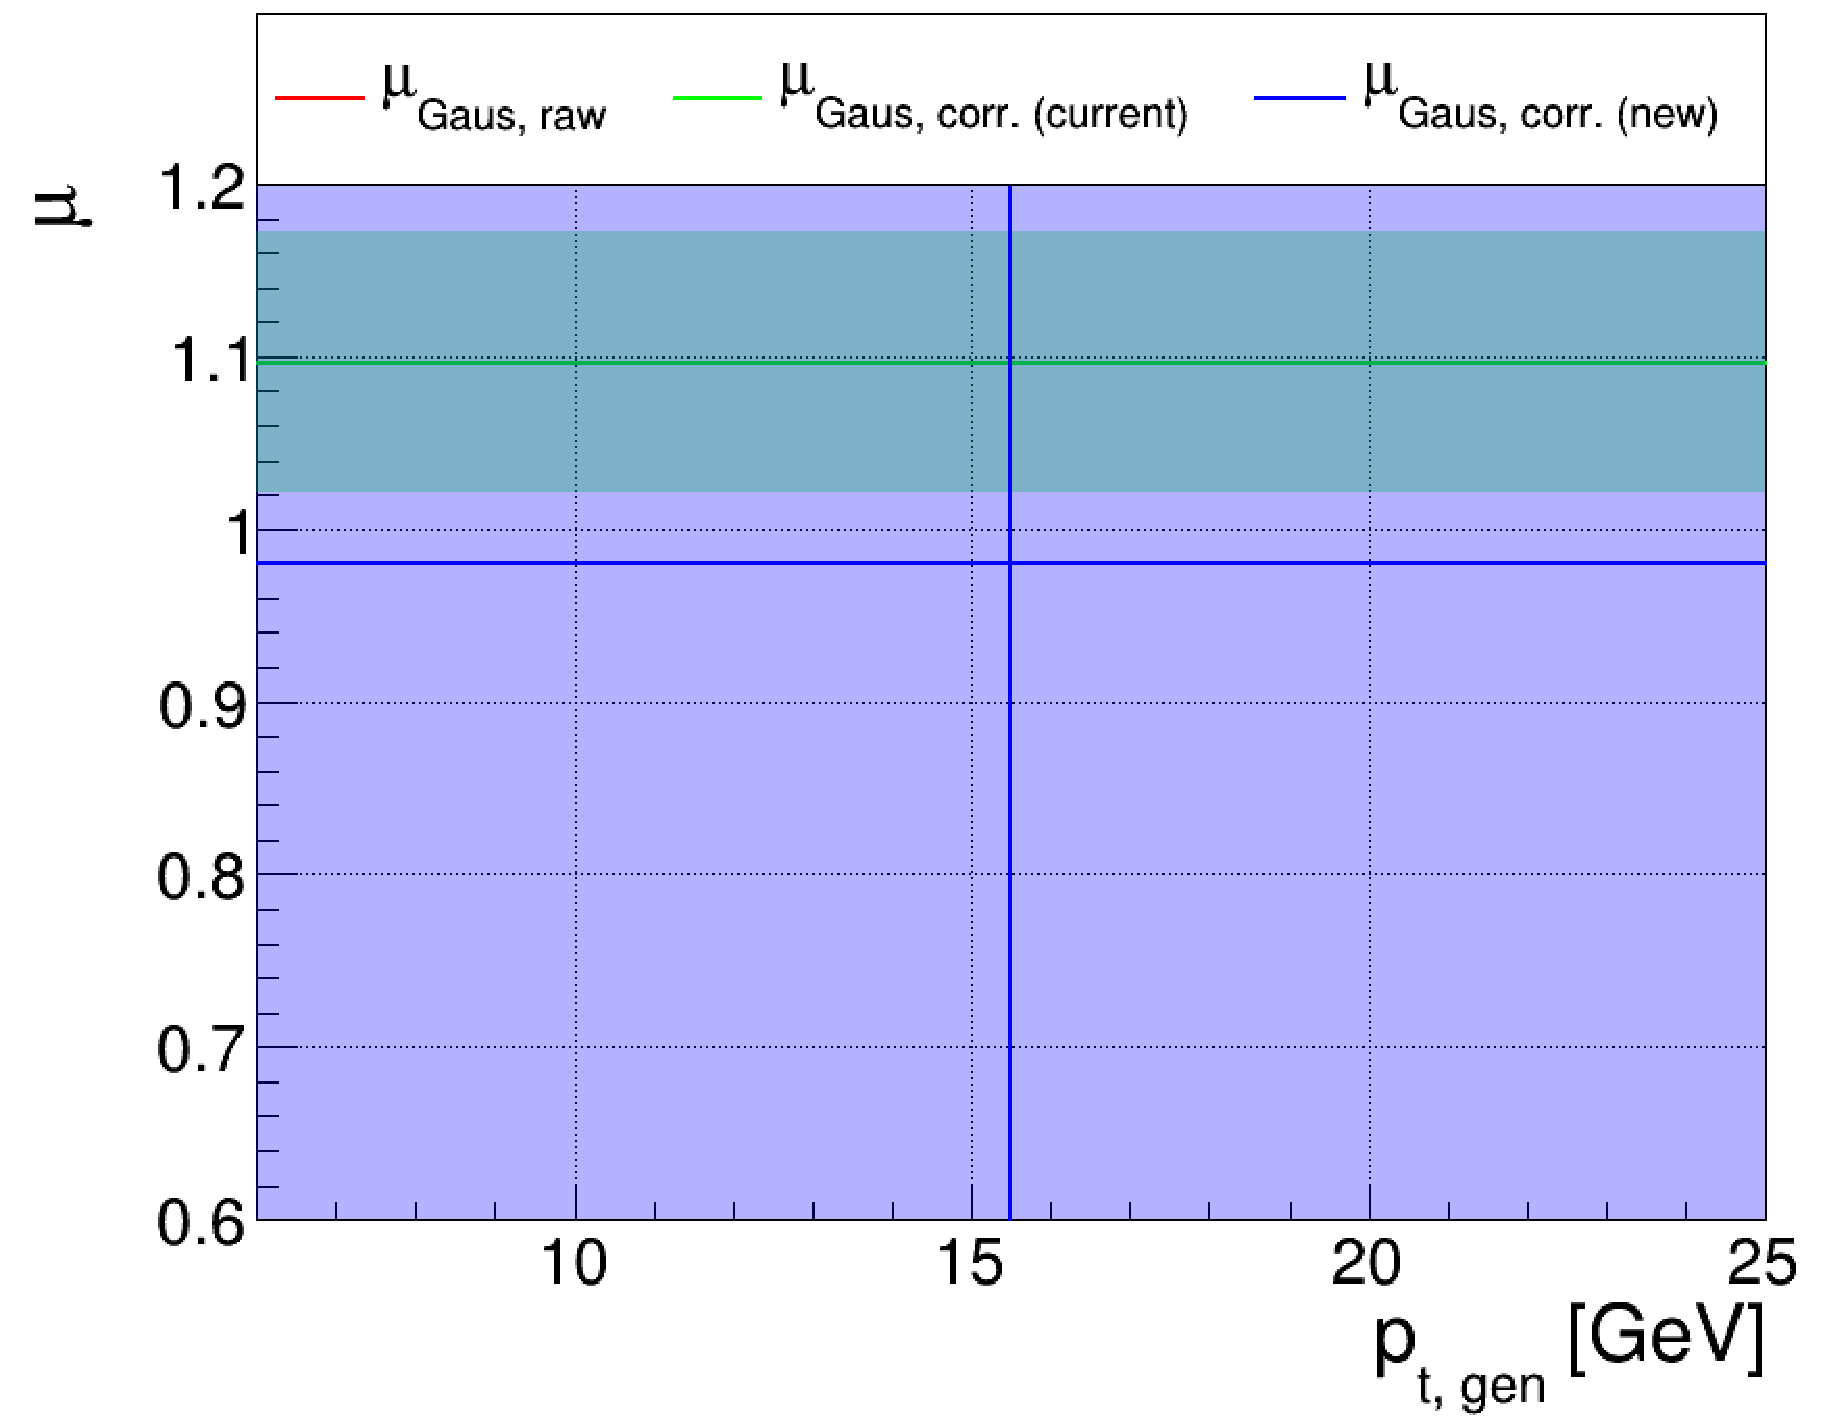
\includegraphics[width=0.495\textwidth]{./plots_pdf/ECAL_plots/plotsPU/EB/ZS/pdf/GENPT/EBZS_GENPT_0006_0025_MuOverBins.pdf}
%% 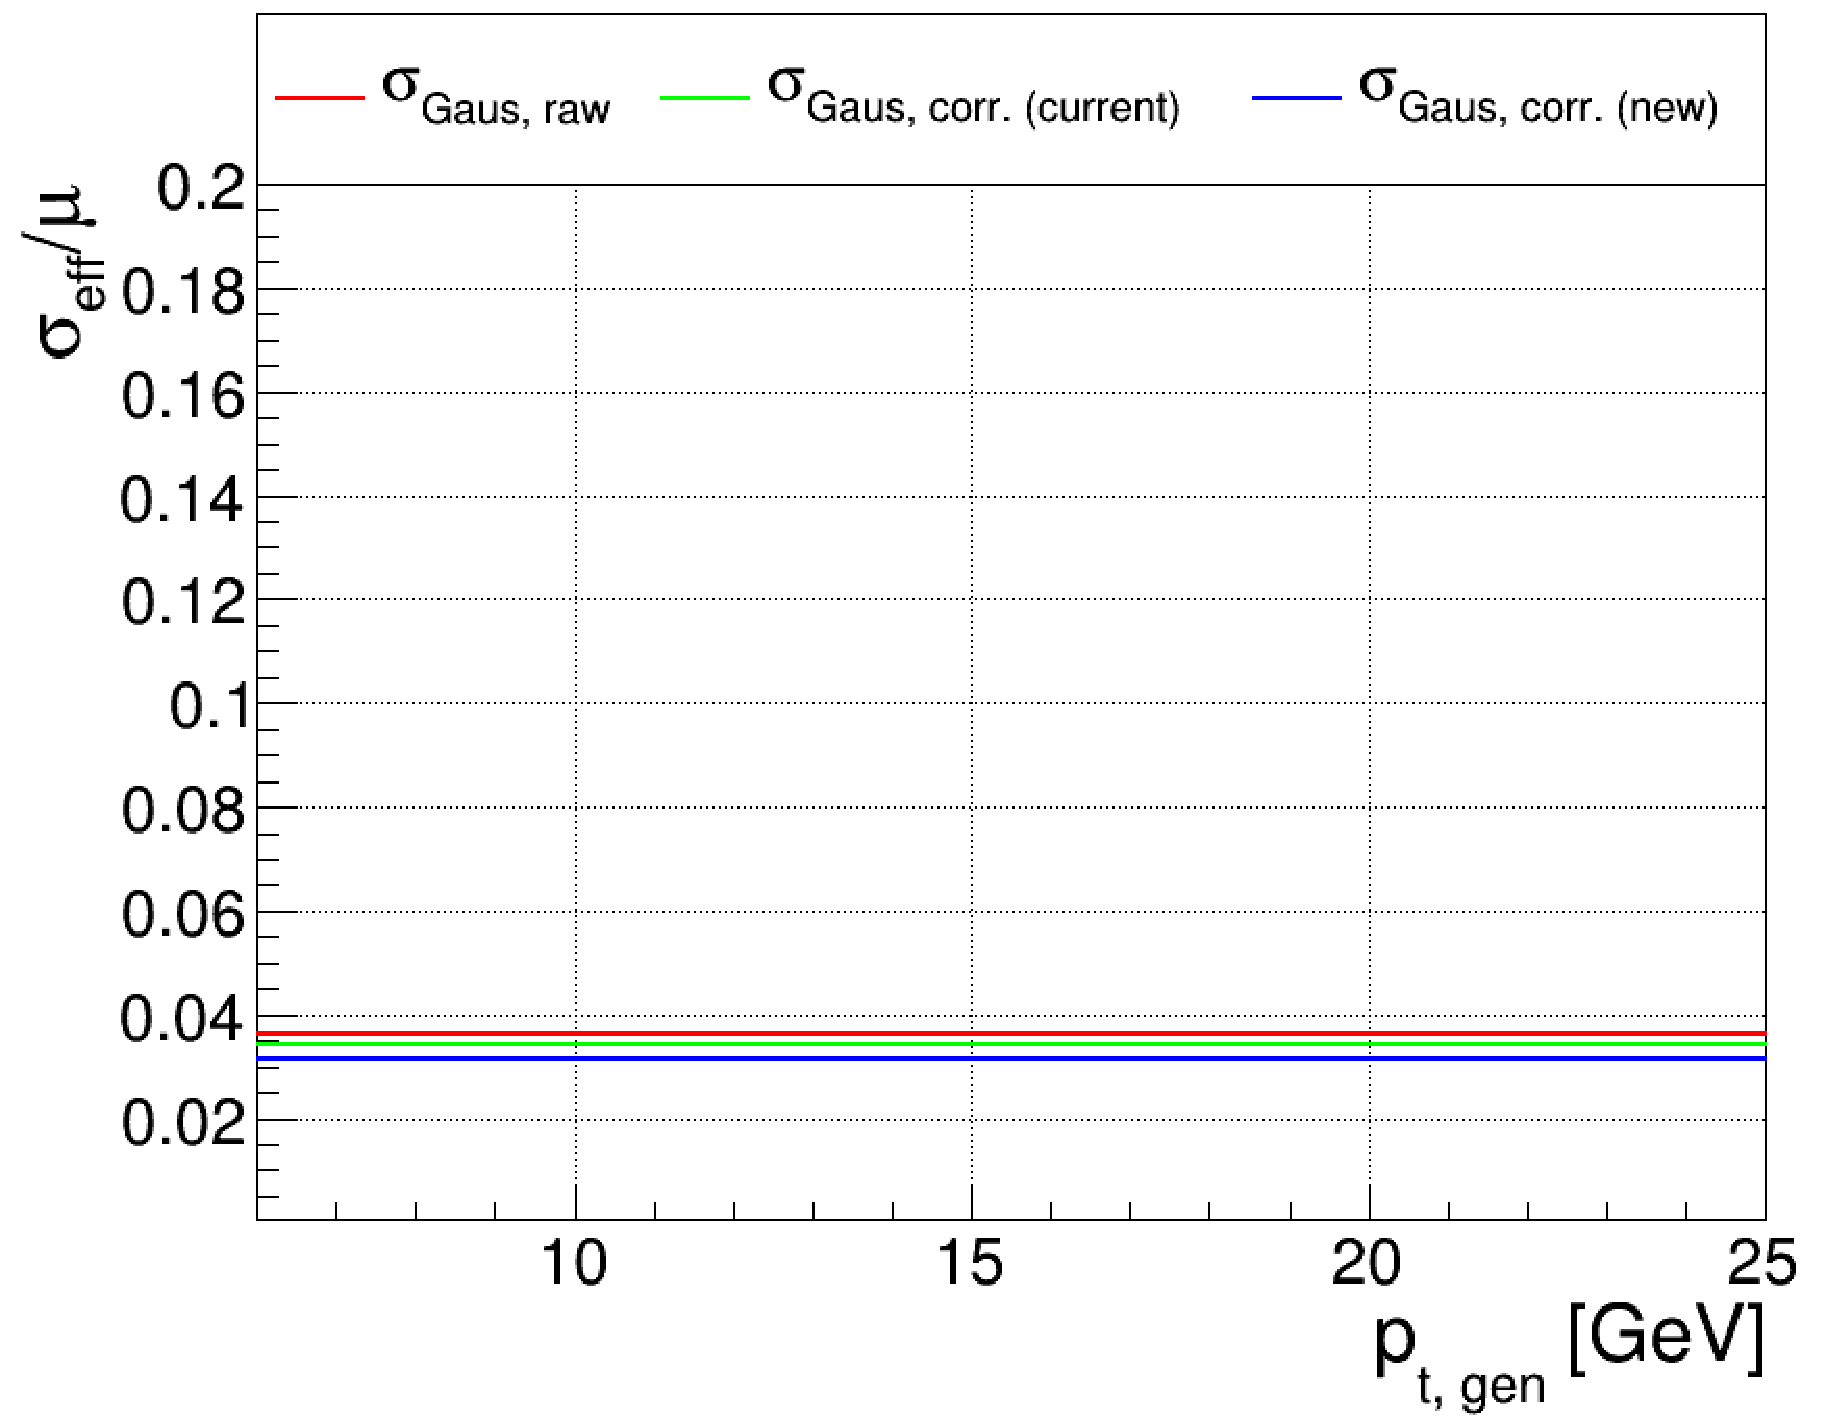
\includegraphics[width=0.495\textwidth]{./plots_pdf/ECAL_plots/plotsPU/EB/ZS/pdf/GENPT/EBZS_GENPT_0006_0025_EffSigmaOverBins.pdf}
%% %\caption{EB - ZS Readout pt 6-25}
%% %\end{figure}
%% %\begin{figure}
%% 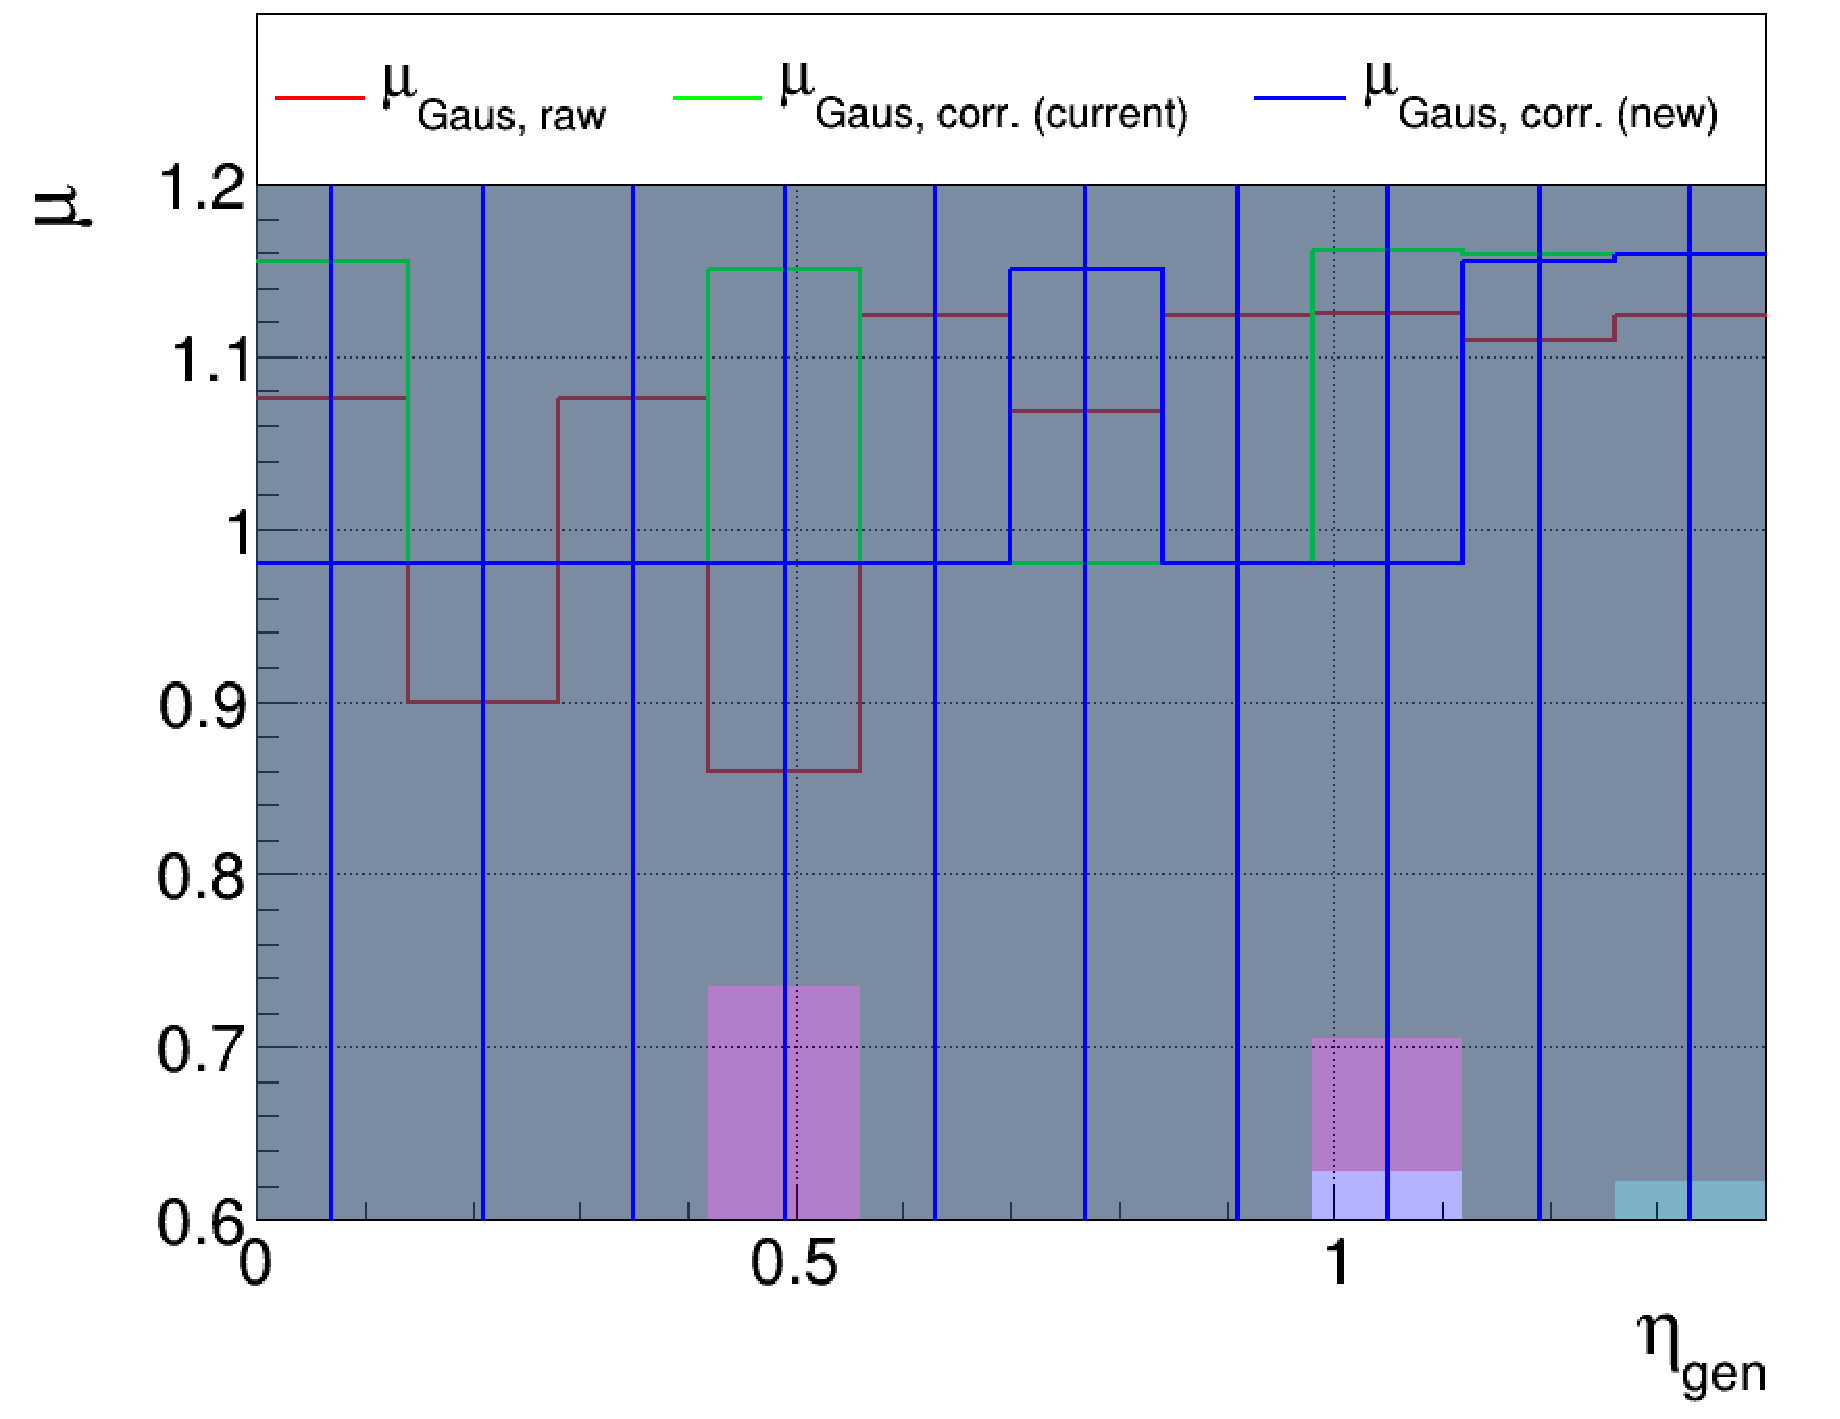
\includegraphics[width=0.495\textwidth]{./plots_pdf/ECAL_plots/plotsPU/EB/ZS/pdf/GENETA/EBZS_GENETA_0006_0025_MuOverBins.pdf}
%% 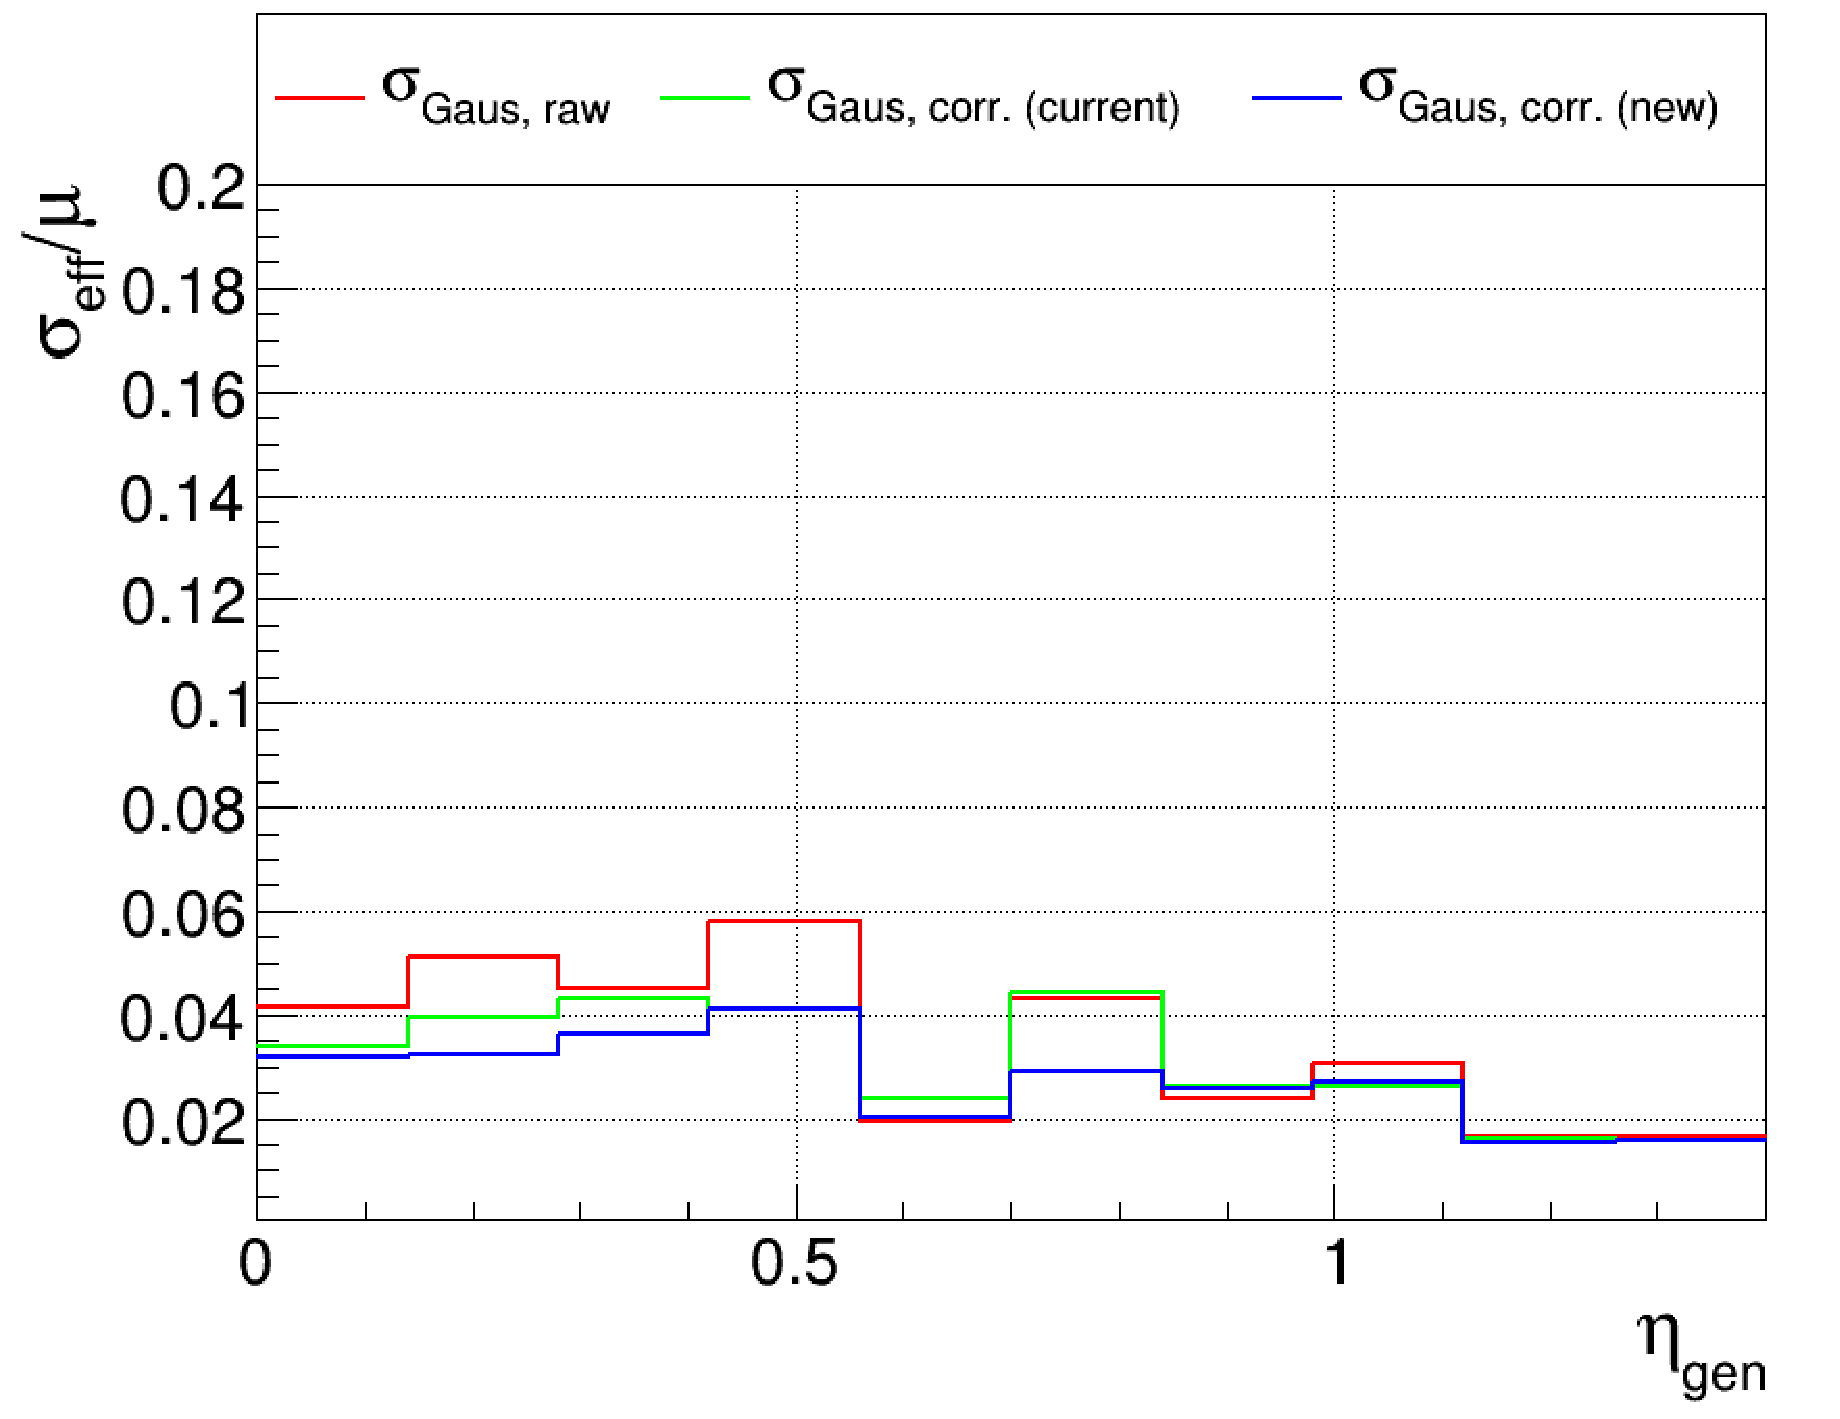
\includegraphics[width=0.495\textwidth]{./plots_pdf/ECAL_plots/plotsPU/EB/ZS/pdf/GENETA/EBZS_GENETA_0006_0025_EffSigmaOverBins.pdf}
%% \caption{EB - ZS Readout \pt 6-25}
%% \end{figure}







\begin{figure}
  %5-20 pt 
\includegraphics[width=0.335\textwidth]{./plots_pdf/ECAL_plots/plotsNOPU/EB/FULL/pdf/GENPT/EBFULL_GENPT_0005_0020_MuOverBins.pdf}
\includegraphics[width=0.3355\textwidth]{./plots_pdf/ECAL_plots/plotsNOPU/EB/FULL/pdf/GENPT/EBFULL_GENPT_0005_0020_EffSigmaOverBins.pdf}

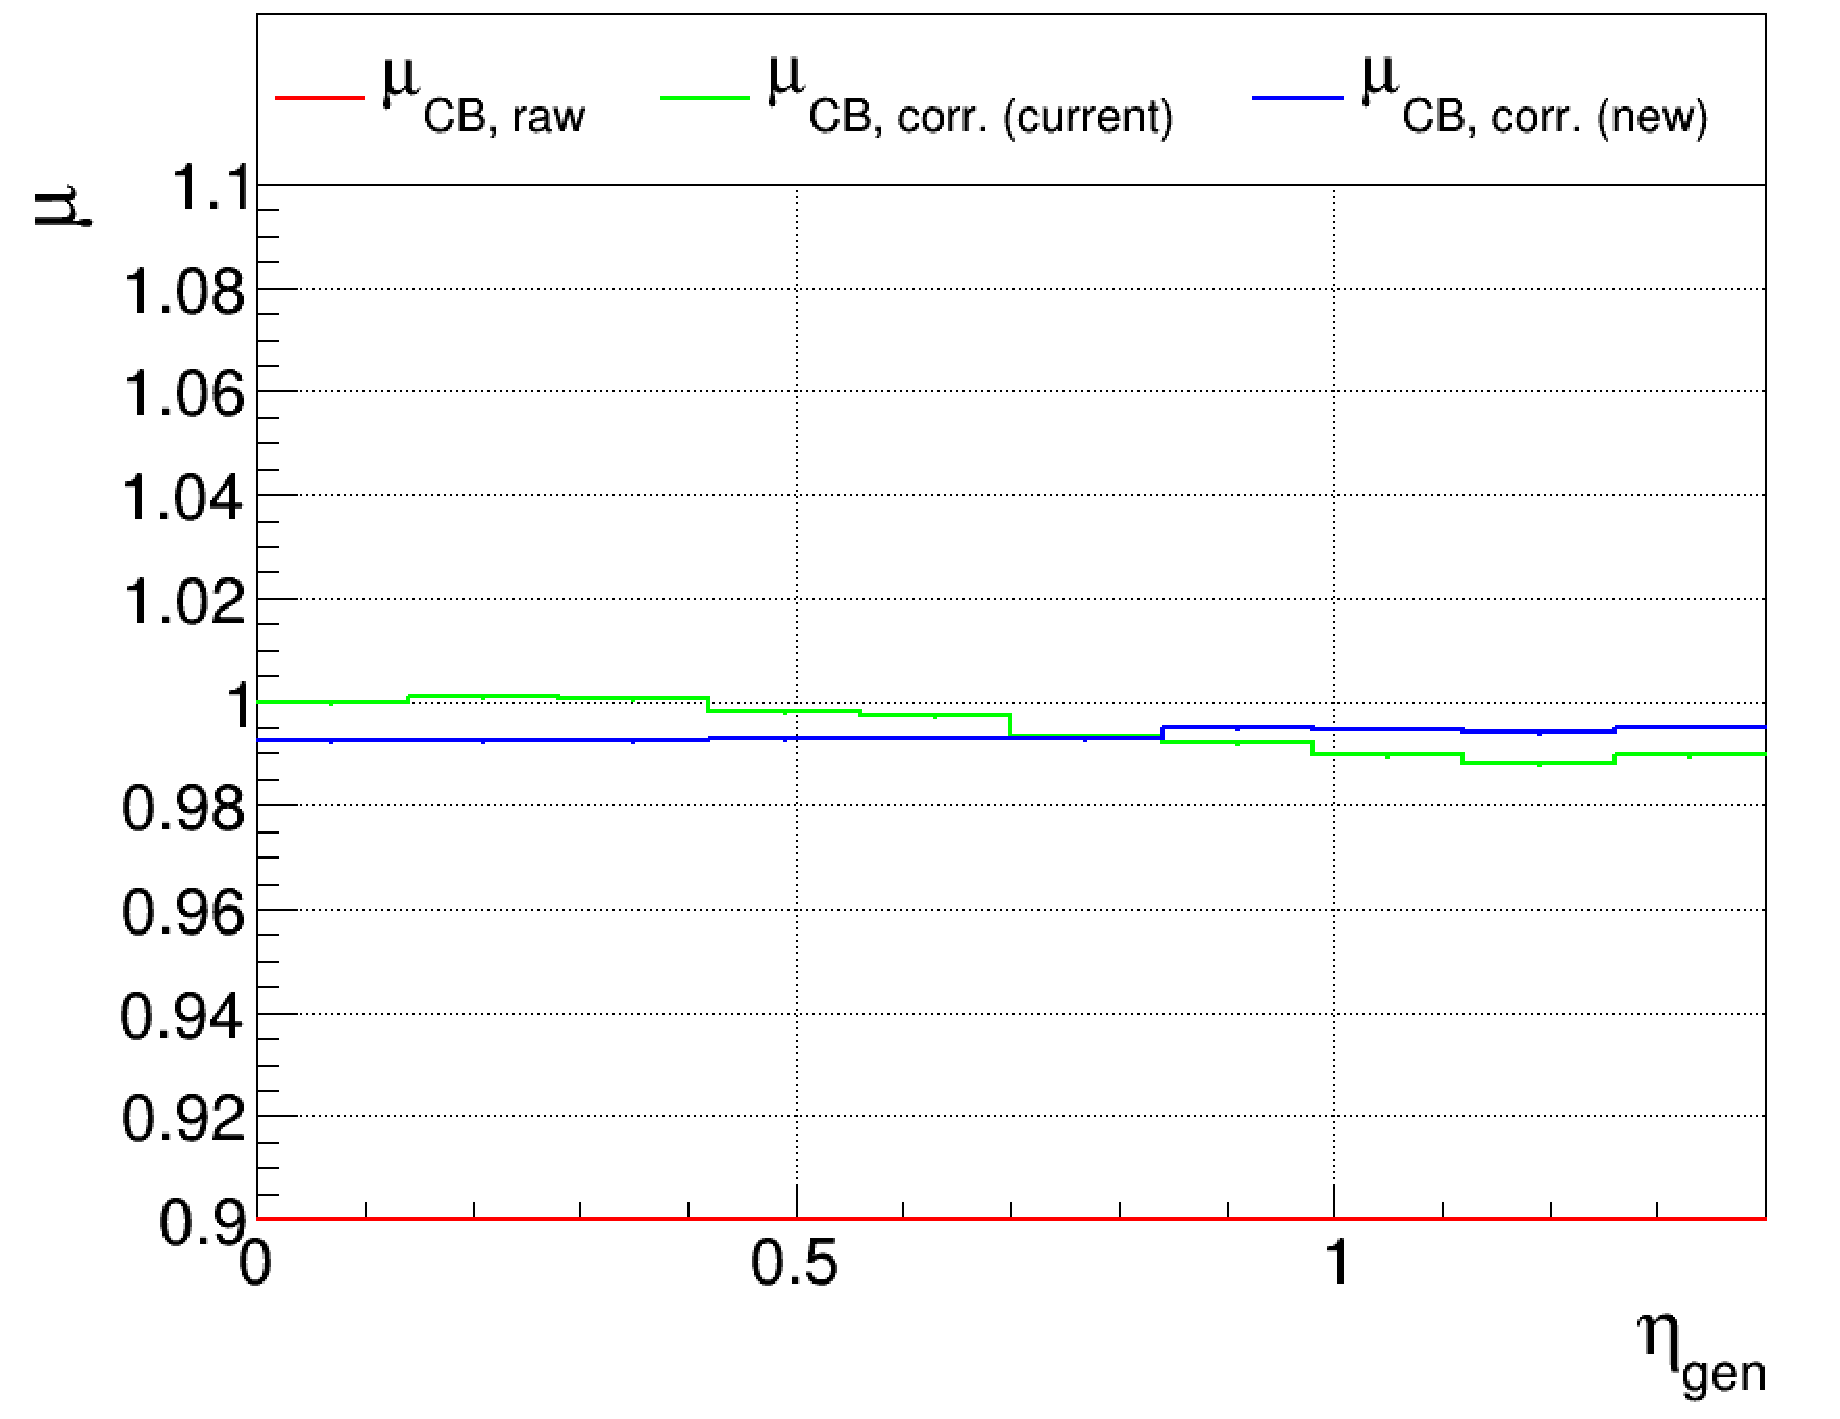
\includegraphics[width=0.495\textwidth]{./plots_pdf/ECAL_plots/plotsNOPU/EB/FULL/pdf/GENETA/EBFULL_GENETA_0005_0020_MuOverBins.pdf}
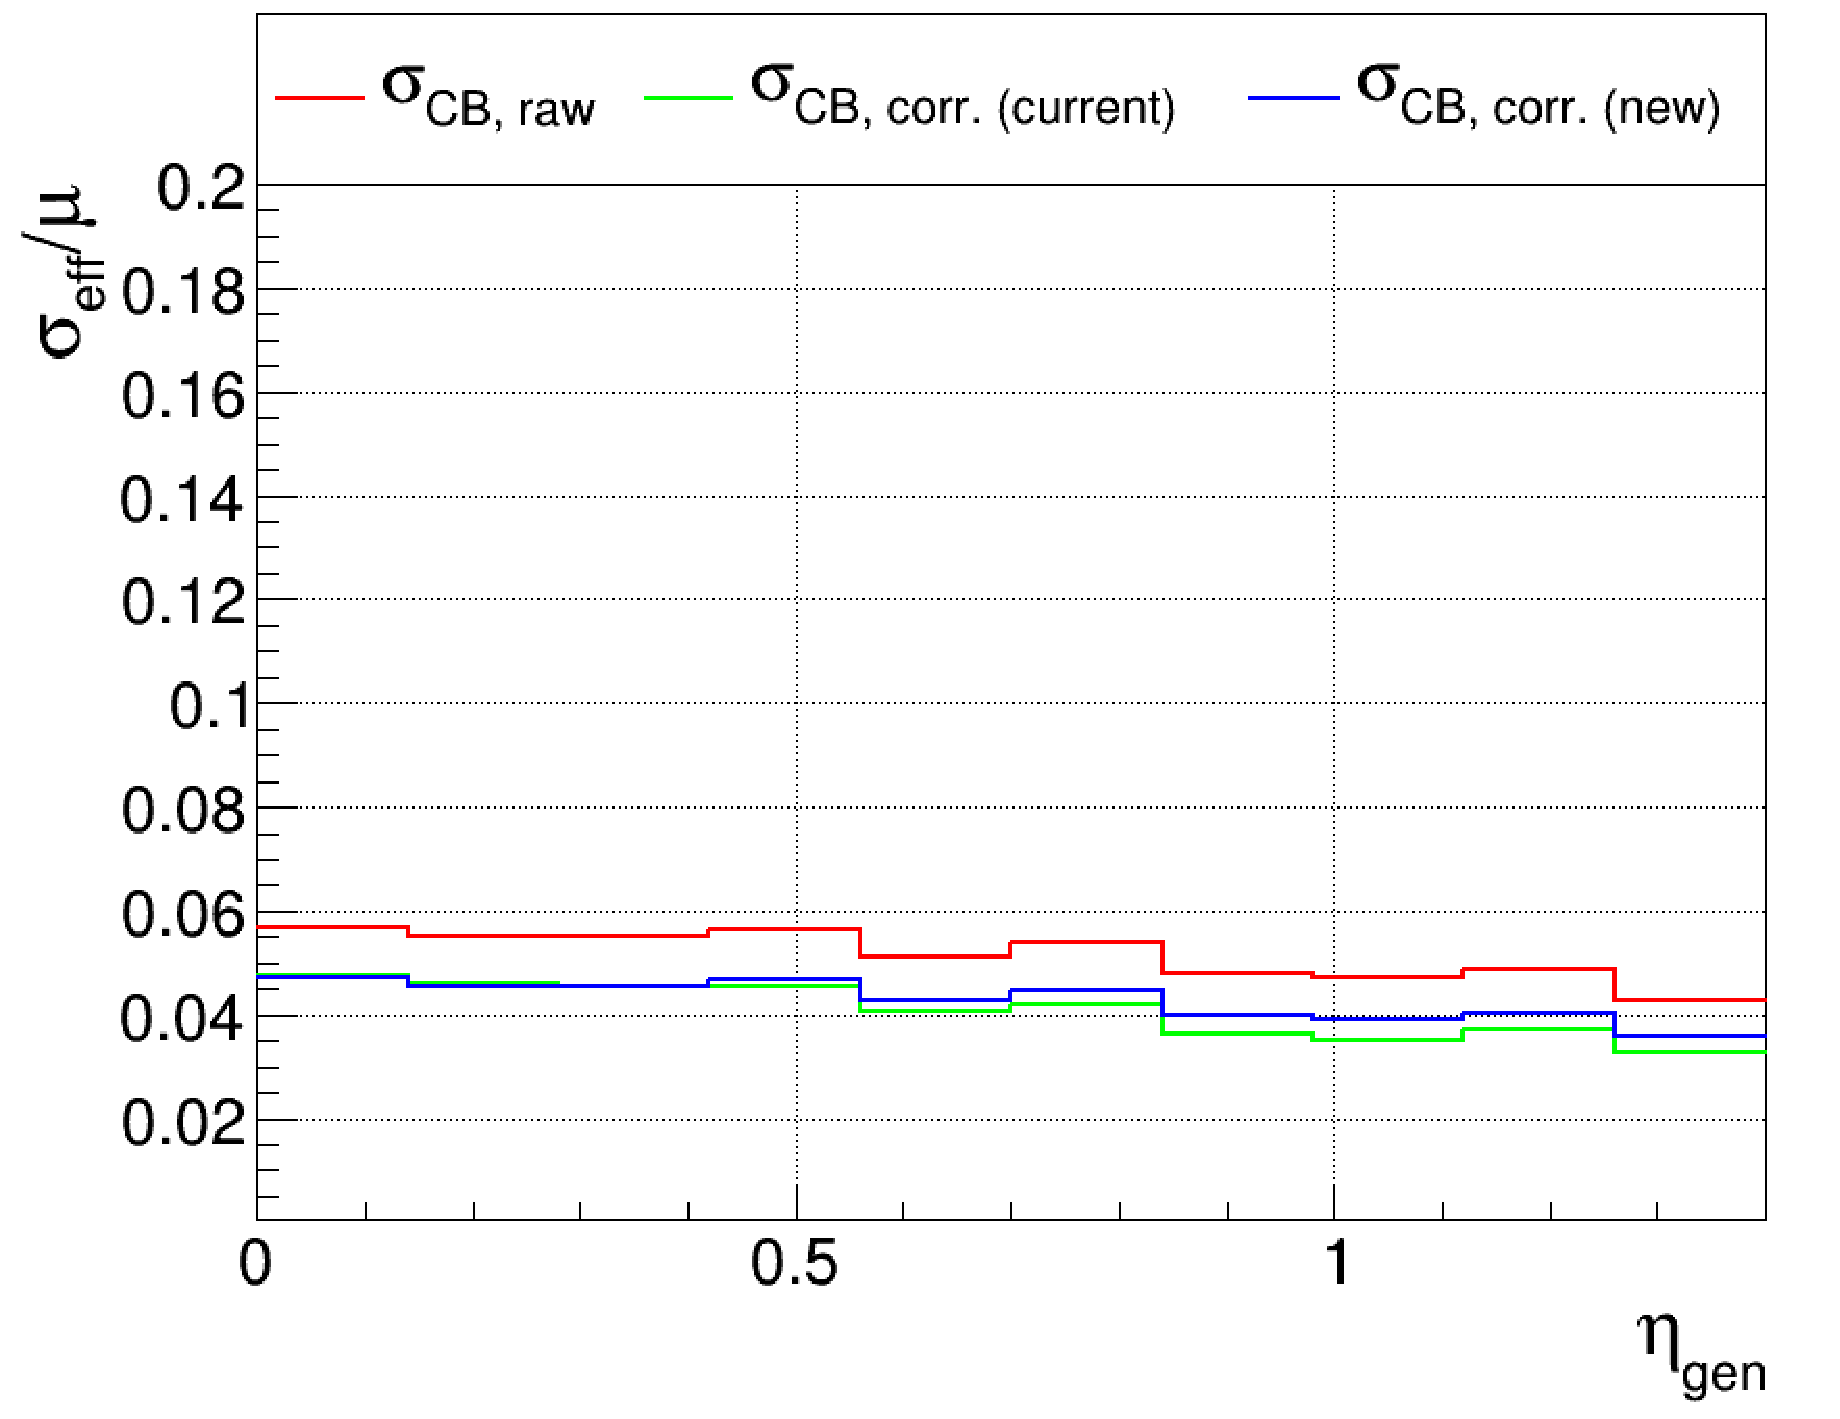
\includegraphics[width=0.495\textwidth]{./plots_pdf/ECAL_plots/plotsPU/EB/FULL/pdf/GENETA/EBFULL_GENETA_0005_0020_EffSigmaOverBins.pdf}
\caption{EB - Full Readout \pt 5-20}

%\begin{figure}
\includegraphics[width=0.495\textwidth]{./plots_pdf/ECAL_plots/plotsNOPU/EB/FULL/pdf/GENPT/EBFULL_GENPT_0020_0100_MuOverBins.pdf}
\includegraphics[width=0.495\textwidth]{./plots_pdf/ECAL_plots/plotsNOPU/EB/FULL/pdf/GENPT/EBFULL_GENPT_0020_0100_EffSigmaOverBins.pdf}

\includegraphics[width=0.495\textwidth]{./plots_pdf/ECAL_plots/plotsNOPU/EB/FULL/pdf/GENETA/EBFULL_GENETA_0020_0100_MuOverBins.pdf}
\includegraphics[width=0.495\textwidth]{./plots_pdf/ECAL_plots/plotsPU/EB/FULL/pdf/GENETA/EBFULL_GENETA_0020_0100_EffSigmaOverBins.pdf}
\caption{EB - Full Readout \pt 20-100}
\end{figure}


\begin{figure}
\includegraphics[width=0.495\textwidth]{./plots_pdf/ECAL_plots/plotsNOPU/EB/FULL/pdf/GENPT/EBFULL_GENPT_0100_0300_MuOverBins.pdf}
\includegraphics[width=0.495\textwidth]{./plots_pdf/ECAL_plots/plotsPU/EB/FULL/pdf/GENPT/EBFULL_GENPT_0100_0300_EffSigmaOverBins.pdf}


\includegraphics[width=0.495\textwidth]{./plots_pdf/ECAL_plots/plotsNOPU/EB/FULL/pdf/GENETA/EBFULL_GENETA_0100_0300_MuOverBins.pdf}
\includegraphics[width=0.495\textwidth]{./plots_pdf/ECAL_plots/plotsNOPU/EB/FULL/pdf/GENETA/EBFULL_GENETA_0100_0300_EffSigmaOverBins.pdf}
\caption{EB - Full Readout \pt 100-300}
\end{figure}




\begin{figure}
\includegraphics[width=0.495\textwidth]{./plots_pdf/ECAL_plots/plotsNOPU/EB/ZS/pdf/GENPT/EBZS_GENPT_0000_0006_MuOverBins.pdf}
\includegraphics[width=0.495\textwidth]{./plots_pdf/ECAL_plots/plotsNOPU/EB/ZS/pdf/GENPT/EBZS_GENPT_0000_0006_EffSigmaOverBins.pdf}

\includegraphics[width=0.495\textwidth]{./plots_pdf/ECAL_plots/plotsNOPU/EB/ZS/pdf/GENETA/EBZS_GENETA_0000_0006_MuOverBins.pdf}
\includegraphics[width=0.495\textwidth]{./plots_pdf/ECAL_plots/plotsNOPU/EB/ZS/pdf/GENETA/EBZS_GENETA_0000_0006_EffSigmaOverBins.pdf}
\caption[]{EB - ZS Readout \pt 0--6\GeV.}
\end{figure}

%% \begin{figure}
%% \includegraphics[width=0.495\textwidth]{./plots_pdf/ECAL_plots/plotsNOPU/EB/ZS/pdf/GENPT/EBZS_GENPT_0006_0025_MuOverBins.pdf}
%% \includegraphics[width=0.495\textwidth]{./plots_pdf/ECAL_plots/plotsNOPU/EB/ZS/pdf/GENPT/EBZS_GENPT_0006_0025_EffSigmaOverBins.pdf}

%% \includegraphics[width=0.495\textwidth]{./plots_pdf/ECAL_plots/plotsNOPU/EB/ZS/pdf/GENETA/EBZS_GENETA_0006_0025_MuOverBins.pdf}
%% \includegraphics[width=0.495\textwidth]{./plots_pdf/ECAL_plots/plotsNOPU/EB/ZS/pdf/GENETA/EBZS_GENETA_0006_0025_EffSigmaOverBins.pdf}
%% \caption[]{EB - ZS Readout \pt 6-25\GeV}
%% \end{figure}






%\subsubsection{ECAL Endcap}

in EE region:
\begin{figure}
\includegraphics[width=0.495\textwidth]{./plots_pdf/ECAL_plots/plotsNoPU/EE/pdf/FULL/GENPT/EEFULL_GENPT_0005_0020_MuOverBins.pdf}
\includegraphics[width=0.495\textwidth]{./plots_pdf/ECAL_plots/plotsNoPU/EE/pdf/FULL/GENPT/EEFULL_GENPT_0005_0020_EffSigmaOverBins.pdf}

\includegraphics[width=0.495\textwidth]{./plots_pdf/ECAL_plots/plotsNoPU/EE/pdf/FULL/GENETA/EEFULL_GENETA_0005_0020_MuOverBins.pdf}
\includegraphics[width=0.495\textwidth]{./plots_pdf/ECAL_plots/plotsNoPU/EE/pdf/FULL/GENETA/EEFULL_GENETA_0005_0020_EffSigmaOverBins.pdf}
\caption{EE - Full Readout \pt 5-20}
%\end{figure}


%\begin{figure}
\includegraphics[width=0.495\textwidth]{./plots_pdf/ECAL_plots/plotsNoPU/EE/pdf/FULL/GENPT/EEFULL_GENPT_0020_0100_MuOverBins.pdf}
\includegraphics[width=0.495\textwidth]{./plots_pdf/ECAL_plots/plotsNoPU/EE/pdf/FULL/GENPT/EEFULL_GENPT_0020_0100_EffSigmaOverBins.pdf}

\includegraphics[width=0.495\textwidth]{./plots_pdf/ECAL_plots/plotsNoPU/EE/pdf/FULL/GENETA/EEFULL_GENETA_0020_0100_MuOverBins.pdf}
\includegraphics[width=0.495\textwidth]{./plots_pdf/ECAL_plots/plotsNoPU/EE/pdf/FULL/GENETA/EEFULL_GENETA_0020_0100_EffSigmaOverBins.pdf}
\caption{EE - Full Readout \pt 20-100}
\end{figure}


\begin{figure}
\includegraphics[width=0.495\textwidth]{./plots_pdf/ECAL_plots/plotsNoPU/EE/pdf/FULL/GENPT/EEFULL_GENPT_0100_0300_MuOverBins.pdf}
\includegraphics[width=0.495\textwidth]{./plots_pdf/ECAL_plots/plotsNoPU/EE/pdf/FULL/GENPT/EEFULL_GENPT_0100_0300_EffSigmaOverBins.pdf}
%\caption{EE - Full Readout pt 100-300}
%\end{figure}
%\begin{figure}
\includegraphics[width=0.495\textwidth]{./plots_pdf/ECAL_plots/plotsNoPU/EE/pdf/FULL/GENETA/EEFULL_GENETA_0100_0300_MuOverBins.pdf}
\includegraphics[width=0.495\textwidth]{.plots_pdf/ECAL_plots/plotsNoPU/EE/pdf/FULL/GENETA/EEFULL_GENETA_0100_0300_EffSigmaOverBins.pdf}
\caption{EE - Full Readout \pt 100-300}
\end{figure}





\begin{figure}
\includegraphics[width=0.495\textwidth]{./plots_pdf/ECAL_plots/plotsNoPU/EE/pdf/ZS/GENPT/EEZS_GENPT_0000_0006_MuOverBins.pdf}
\includegraphics[width=0.495\textwidth]{./plots_pdf/ECAL_plots/plotsNoPU/EE/pdf/ZS/GENPT/EEZS_GENPT_0000_0006_EffSigmaOverBins.pdf}

\includegraphics[width=0.495\textwidth]{./plots_pdf/ECAL_plots/plotsNoPU/EE/pdf/ZS/GENETA/EEZS_GENETA_0000_0006_MuOverBins.pdf}
\includegraphics[width=0.495\textwidth]{./plots_pdf/ECAL_plots/plotsNoPU/EE/pdf/ZS/GENETA/EEZS_GENETA_0000_0006_EffSigmaOverBins.pdf}
\caption[$\mu$ ($\sigma_\mathrm{eff}$) vs \pt of PF ECAL cluster - EE ZS readout NoPU scenario]{Mean response (resolution) defined by Raw PF ECAL clusters (red), the calibration derived earlier in Ru\
n3 based on 126X (green), and the new correction from 2024 simulation sample based on 133X (blue).\pt 0--6\GeV in EE region ZS Readout NOPU scenario.}
\end{figure}

%% %\begin{figure}
%% \includegraphics[width=0.495\textwidth]{./plots_pdf/ECAL_plots/plotsNoPU/EE/pdf/ZS/GENPT/EEZS_GENPT_0006_0025_MuOverBins.pdf}
%% \includegraphics[width=0.495\textwidth]{./plots_pdf/ECAL_plots/plotsNoPU/EE/pdf/ZS/GENPT/EEZS_GENPT_0006_0025_EffSigmaOverBins.pdf}
%% %\caption{EE - ZS Readout pt 6-25}
%% %\end{figure}
%% %\begin{figure}
%% \includegraphics[width=0.495\textwidth]{./plots_pdf/ECAL_plots/plotsNoPU/EE/pdf/ZS/GENETA/EEZS_GENETA_0006_0025_MuOverBins.pdf}
%% %\includegraphics[width=0.495\textwidth]{./ECAL_plots/plotsNoPU/EE/pdf/ZS/GENETA/EEZS_GENETA_0006_0025_EffSigmaOverBins.pdf}
%% \caption{EE - ZS Readout \pt 6-25}
%% \end{figure}




\begin{figure}
\includegraphics[width=0.495\textwidth]{./plots_pdf/ECAL_plots/plotsPU/EE/FULL/pdf/GENPT/EEFULL_GENPT_0005_0020_MuOverBins.pdf}
\includegraphics[width=0.495\textwidth]{./plots_pdf/ECAL_plots/plotsPU/EE/FULL/pdf/GENPT/EEFULL_GENPT_0005_0020_EffSigmaOverBins.pdf}
\includegraphics[width=0.495\textwidth]{./plots_pdf/ECAL_plots/plotsPU/EE/FULL/pdf/GENPT/EEFULL_GENPT_0020_0100_MuOverBins.pdf}
\includegraphics[width=0.495\textwidth]{./plots_pdf/ECAL_plots/plotsPU/EE/FULL/pdf/GENPT/EEFULL_GENPT_0020_0100_EffSigmaOverBins.pdf}
\includegraphics[width=0.495\textwidth]{./plots_pdf/ECAL_plots/plotsPU/EE/FULL/pdf/GENPT/EEFULL_GENPT_0100_0300_MuOverBins.pdf}
\includegraphics[width=0.495\textwidth]{./plots_pdf/ECAL_plots/plotsPU/EE/FULL/pdf/GENPT/EEFULL_GENPT_0100_0300_EffSigmaOverBins.pdf}

\caption [$\mu$ ($\sigma_\mathrm{eff}$) vs \pt of PF ECAL cluster - EE full readout PU scenario]{Mean response (resolution) defined by Raw PF ECAL clusters (red), the calibration derived earlier in Ru\
n3 based on 126X (green), and the new correction from 2024 simulation sample based on 133X (blue). (top) low \pt, (middle) mid \pt, (bottom) high \pt in EE region full readout PU scenario.}
\label{fig:PU_EEFULL_pt}
\end{figure}


\begin{figure}
\includegraphics[width=0.495\textwidth]{./plots_pdf/ECAL_plots/plotsPU/EE/FULL/pdf/GENETA/EEFULL_GENETA_0005_0020_MuOverBins.pdf}
\includegraphics[width=0.495\textwidth]{./plots_pdf/ECAL_plots/plotsPU/EE/FULL/pdf/GENETA/EEFULL_GENETA_0005_0020_EffSigmaOverBins.pdf}
\includegraphics[width=0.495\textwidth]{./plots_pdf/ECAL_plots/plotsPU/EE/FULL/pdf/GENETA/EEFULL_GENETA_0020_0100_MuOverBins.pdf}
\includegraphics[width=0.495\textwidth]{./plots_pdf/ECAL_plots/plotsPU/EE/FULL/pdf/GENETA/EEFULL_GENETA_0020_0100_EffSigmaOverBins.pdf}
\includegraphics[width=0.495\textwidth]{./plots_pdf/ECAL_plots/plotsPU/EE/FULL/pdf/GENETA/EEFULL_GENETA_0100_0300_MuOverBins.pdf}
\includegraphics[width=0.495\textwidth]{./plots_pdf/ECAL_plots/plotsPU/EE/FULL/pdf/GENETA/EEFULL_GENETA_0100_0300_EffSigmaOverBins.pdf}


\caption [$\mu$ ($\sigma_\mathrm{eff}$) vs $\eta$ of PF ECAL cluster - EE Full readout PU scenario]{Mean response (resolution) defined by Raw PF ECAL clusters (red), the calibration derived earlier in\
 Run3 based on 126X (green), and the new correction from 2024 simulation sample based on 133X (blue). (top) low $\eta$, (middle) mid $\eta$, (bottom) high $\eta$ in EE region Full readout PU scenario.}
\label{fig:PU_EEFULL_eta}
\end{figure}

\begin{figure}
\includegraphics[width=0.495\textwidth]{./plots_pdf/ECAL_plots/plotsPU/EE/ZS/pdf/GENPT/EEZS_GENPT_0000_0006_MuOverBins.pdf}
\includegraphics[width=0.495\textwidth]{./plots_pdf/ECAL_plots/plotsPU/EE/ZS/pdf/GENPT/EEZS_GENPT_0000_0006_EffSigmaOverBins.pdf}

\includegraphics[width=0.495\textwidth]{./plots_pdf/ECAL_plots/plotsPU/EE/ZS/pdf/GENETA/EEZS_GENETA_0000_0006_MuOverBins.pdf}
\includegraphics[width=0.495\textwidth]{./plots_pdf/ECAL_plots/plotsPU/EE/ZS/pdf/GENETA/EEZS_GENETA_0000_0006_EffSigmaOverBins.pdf}

\caption[$\mu$ ($\sigma_\mathrm{eff}$) vs. \pt of PF ECAL cluster - EE ZS readout PU scenario]{Mean response (resolution) defined by raw PF ECAL clusters (red), the calibration derived earlier in Run~3 based on 126X (green), and the new correction from the 2024 simulation sample based on 133X (blue).\pt 0--6\GeV in EE region ZS readout PU scenario.}
\label{fig:PU_EEZS}
\end{figure}

%% %\begin{figure}
%% \includegraphics[width=0.495\textwidth]{./plots_pdf/ECAL_plots/plotsPU/EE/ZS/pdf/GENPT/EEZS_GENPT_0006_0025_MuOverBins.pdf}
%% \includegraphics[width=0.495\textwidth]{./plots_pdf/ECAL_plots/plotsPU/EE/ZS/pdf/GENPT/EEZS_GENPT_0006_0025_EffSigmaOverBins.pdf}
%% %\caption{EE - ZS Readout pt 6-25}
%% %\end{figure}
%% %\begin{figure}
%% \includegraphics[width=0.495\textwidth]{./plots_pdf/ECAL_plots/plotsPU/EE/ZS/pdf/GENETA/EEZS_GENETA_0006_0025_MuOverBins.pdf}
%% \caption{EE - ZS Readout \pt 6-25}
%% \end{figure}








\subsection{HLT vs offline PF ECAL cluster}

(connect to PF chapter where where we mentioned offline PF)
(also mention the procution of a new ntuple that containes HLT information) 

first for NoPU samples

\begin{figure}
\includegraphics[width=0.495\textwidth]{./plots_pdf/ECAL_plots/Prod6/NoPU/H_GenPi_Pt_vs_RespE.pdf}
\includegraphics[width=0.495\textwidth]{./plots_pdf/ECAL_plots/Prod6/NoPU/H_GenPi_Eta_vs_RespE.pdf}
\caption [HLT vs offline PF ECAL cluster - NoPU scenario]{(left) ratio of the offline to the online PF ECAL cluster vs $\pt$ in GeV. (right) ratio of the offline PF ECAL cluster to the online PF ECAL cluster vs $\eta$. NoPU scenario.}
\label{fig:NoPU_ECAL_Offline_vs_Online_E}
\end{figure}

\begin{figure}
\includegraphics[width=0.495\textwidth]{./plots_pdf/ECAL_plots/Prod6/NoPU/H_GenPi_Pt_vs_RespCE.pdf}
\includegraphics[width=0.495\textwidth]{./plots_pdf/ECAL_plots/Prod6/NoPU/H_GenPi_Eta_vs_RespCE.pdf}
\caption[HLT vs offline calibrated PF ECAL cluster - NoPU scenario]{(left) ratio of the offline to the online calibrated PF ECAL cluster vs $\pt$ in GeV. (right) ratio of the offline PF ECAL cluster to the online calibrated PF ECAL cluster vs $\eta$. NoPU scenario.}
\label{fig:NoPU_ECAL_Offline_vs_Online_CE}
\end{figure}                                                                                                                                                                       



Second for PUU samples
\begin{figure}
\includegraphics[width=0.495\textwidth]{./plots_pdf/ECAL_plots/Prod6/PU/H_GenPi_Pt_vs_RespE.pdf}
%\caption{(PF cluster offline E / PFC online E) vs pt}                                                                 
\includegraphics[width=0.495\textwidth]{./plots_pdf/ECAL_plots/Prod6/PU/H_GenPi_Eta_vs_RespE.pdf}
\caption{(PF cluster offline E / PFC online E)}
\label{fig:PU_ECAL_Offline_vs_Online_E}
\end{figure}

\begin{figure}
\includegraphics[width=0.495\textwidth]{./plots_pdf/ECAL_plots/Prod6/PU/H_GenPi_Pt_vs_RespCE.pdf}
%\caption{(PF cluster offline E corrected / PFC online E corrected) vs pt}                                             
\includegraphics[width=0.495\textwidth]{./plots_pdf/ECAL_plots/Prod6/PU/H_GenPi_Eta_vs_RespCE.pdf}
\caption{(PF cluster offline E corrected / PFC online E corrected)}
\label{fig:PU_ECAL_Offline_vs_Online_CE}
\end{figure}       


%=====================================
\chapter{Hadronic Cluster Calibration} 
%\chapter{Hadronic Cluster Calibration Using Graph Neural Network}
%\label{chapter:ch4}
%%% Ch4:Hadronic Cluster Calibration UsinAg Graph Neural Network%% 

\section{Introduction to Graph Neural Network}
GNN is a type of NN that is used to process data that can be represented as graphs.
% https://en.wikipedia.org/wiki/Graph_neural_network
% check: A Gentle Introduction to Graph Neural Networks https://distill.pub/2021/gnn-intro/
% check: Basic Understanding of Neural Network Structure https://medium.com/@sarita_68521/basic-understanding-of-neural-network-structure-eecc8f149a23
% check: Epochs, Batch Size, Iterations https://www.sabrepc.com/blog/Deep-Learning-and-AI/Epochs-Batch-Size-Iterations
%=================================================

% Where GNN's are used in CMS?
%% For Calorimetry, In both ECAL & HCAL.

% what are NN?
% what are GNN?

% where GNN can be used in ECAL?
%% for superclustering "Particle reconstruction", particle identification (identify the flavor of the particle), energy regression. 

% when do we perform energy correction?
%% after superclusters are formed, energy corrections are applied.
%% this correction account for the energy lost in gaps and upstream material .. etc
%% currently this calibration is done using BDT with semiparametric regression. (this work is covered in previous chapter)
%% new ML algorithm developed DRN (to use low level inputs (rechits) instead of high level inputs (describe EM showers))

% Energy corrections using Dynamic Reduction Network?
%% input features (rechits) are transformed into high dimensional latent space.
%% Then graphs are dynamically generated in the latent space.
%% the graph convolution are performed (includes message passing)
%% the info is aggregated over the graph using clustering and pooling.
%% => input: Rechit features (E,x,y,z) => output: Predict probability density of energy correction value.
%% slide 16 has resolution plot that compare BDT to DRN calibration. (using photon gun simulation with ideal detector calibration)

% source: ML for calorimetry by Polina simkina

%================================================

% DRN architecture overview:
%..........................
%% 1. input: Rechits => inputNet (FCNN) *Fully Convolutional Network?*
%% 2. => Graph Generation (KNN) => EdgeConv => calculate edge weights => graph clustering (Graclus) => graph pooling (add)
%% 3. Global pool (max)
%% 4. outputNet => output (E pred)

% Training target?
%% minimize loss - [(E true- E pre)^/E true]

% DRN training parapmeters?
%% Input layers: 3
%% aggregation layers: 2
%=> *An aggregation layer is a crucial part of network architecture that connects the access layer to the core layer.
%=> It's also known as the distribution layer.
%=> The aggregation layer's main purpose is to increase network scalability and manage traffic*
%=> source: https://www.sciencedirect.com/topics/computer-science/aggregation-layer#:~:text=The%20aggregation%20layer%20is%20defined,with%20vPC%20in%20computer%20networks.
%% message passing layers:3
%=> *Message passing layers are permutation-equivariant layers mapping a graph into an updated representation of the same graph.
%=> Formally, they can be expressed as message passing neural networks (MPNNs)* source: https://en.wikipedia.org/wiki/Graph_neural_network#Message_passing_layers
%% output layers: 2, *why 2 instead of 1??*
%% hidden dimension: 64
%% batch size: 100
%=> Batch Size is among the important hyperparameters in Machine Learning.
%=> It is the hyperparameter that defines the number of samples to work through before updating the internal model parameters.
%=> source: https://medium.com/geekculture/how-does-batch-size-impact-your-model-learning-2dd34d9fb1fa
%% optimizer w/ constant learning reate of 0.001 AdamW
%=> check video https://www.youtube.com/watch?v=oWZbcq_figk to learn more about AdamW
%% model parameters: 62405
%% total events # training, # validation. 

% Rechits (input): slide 11
%.................
% where do we get the PF Rechits? 
%% for each event we get the desired PF candidate. then we get the corresponding elements in its PFBlock (tracks/cluster).
%% then we collect all the PFElemnets of pfc which formed form eithr ECAL or HCAL.
%% then from each element we get the corresponding cluster reference & associated "hitAndFractions" = RecHits => input in ML algo.
% what are the input features?
%% Rechit position (x vs y) (z, Energy)

% note: for diagnostic checks we compare total rechit energy
% Raw energy (total raw pf)  , Gen level energy (total true pf) - X axis
% ?? - Y axis (slide 13) ?? frequency ?
% ** still don't understand plots in slide 14 ( is it corrected vs True? , color? frequency?)

% Summary
%........
%% Hadron Calibration is challenging.
%% The used input for ML modle is Rechits which are a PF element.
%% Calibration for (charged PF hadrons) using DRN & Chi squar method is done.
%% more improvement in the response for EH tha  H. 

% source: PF hadron cluster calibration 26/2/2024
%================================================

% What are the technical details of the calibration data,
%........................................................
%% centrally generated (true, raw) and reconstructed single pion (- charged hadron) samples.
%% In CMSSW version 12_6_4 (We used) , GT (global target) 126X_mcRun3_2023_forPU65_v4 (after ECAL corrections)
%% E range (2-200) (200-500) GeV (FlatRandomEGunProducer ) + |eta|<3  & |Phi| < 3.14 range 
%%%*This Particle Gun will generate one or more particles,
%%%all coming from the same vertex (0,0,0) and uniformly distributed in the user-specified phi-, eta- and energy-range*
% source: https://twiki.cern.ch/twiki/bin/view/CMSPublic/SWGuideParticleGuns

% How calibration using chi squre method is done?
%................................................

% How is it done using DRN?
%.........................

% what is the motivation for offline calibration?
%...............................................
% when plotting the resolution vs true energy for EH hadrons we can see that
%% the resolution is non linear
%%%* A "non-linear resolution" in calorimetry calibration refers to a method where the calibration constants applied to a calorimeter's signal
%%% are not a simple linear function of energy, meaning the relationship between the measured signal and the actual deposited energy is not a straight line,
%%% but instead exhibits curvature, requiring a more complex mathematical model to accurately convert signals to energy values;
%%% this is often necessary to account for inherent non-linearities in the calorimeter response,
%%% like variations in shower development at different energy levels or non-uniformities within the detector itself. (AI answer google)

%%%*a "calorimeter response" refers to the measurable signal produced by a calorimeter when a particle is completely absorbed within it,
%%% essentially representing the energy of the incident particle as a detectable output,
%%% typically in the form of light or electrical charge generated by the secondary particles produced in the particle shower;
%%% it is essentially how much signal is generated per unit of energy deposited in the calorimeter, and can vary depending on the type of particle being absorbed.*

% => check more general info about calorimeters see talk Calorimeters Energy measurement

% using  Chi square method, what are the energy/ Pseudorapidity dependent calibrationss?
% .........................................................................
%%%* In statistics, minimum chi-square estimation is a method of estimation of unobserved quantities based on observed data.
% => source: https://en.wikipedia.org/wiki/Minimum_chi-square_estimation
%% Energy dependent calibration: slide 5 
%% EH hadrons: E(corrected):a* E(raw Ecal) + b*E(raw Hcal) + O(EH) 
%% H hadrons: E(corrected): c*E(raw Hcal) + O(H)
%%% * coeffiecent O: accounts for the energy lost beacuse of the energy thresholds of the clustering algorithm.
%%% * coeffiecent a,b,c could be estimated using a large sample of simulated particles
%%% after getting the coeffiecents we can apply the corrections on the raw ECAL & HCAL energies. 


% types of calibration?
%.....................
% => check pg 47 Source: calorimetry for particle physics

%%%* Absolute calibration of a calorimeter is a process that determines the constants needed to convert raw ADC codes into energy depositions
%%% in the calorimeter counters. The goal is to ensure accurate measurements of heat changes in chemical reactions or physical processes. (AI answer google)


%%%%%%%%%%%%%%%%%%%%%%%%%%%%%%%%%%%%%%%%%%%%%%%%%%% 
\section{HCAL Cluster Calibration using GNN}

Hadronic showers in the CMS detector have both electromagnetic and hadronic components.

These showers are not dully contained in the ECAL but extend to HCAL.

The detector response is different for EM and HAD componenets which lead to non linear energy response.

The reconstructed energy of hadrons is the sum if all reconstructed hits (offline, PF reconstruct the RAW data) from the ECAL and HCAL.

For a given bin of ture energy (PF also reconstruct generated data or MC data):

by fitting the distribution of total RAW energy with Gaussian we obtain mu and std deviation then use them to get:

Resolution (std/mu) : which is a measure of accuracy

and Response [(mu/E true) -1] : which is measurement of precision. (we can see that is not linear)

Energy Reconstruction using conventional method (chi square) vs DRN (based on GNN).

The work in this thesis is done for Run3 data. 


\subsection{Strategy}


\subsection{Samples used and Training Details}

Include DRN architecture overview here. We could include the Training target.  

DRN training parameters. this include: Inpute layers (3) .. etc.

Sample details: centrally produced GEN-SIM-RAW (two momentum range) and privately reconstructed in CMSSW.

Rechits used as input. (we could expand more on this detail)

\subsection{Validation}

80\% of the dataset used for taining and 20\% for validation.  

% source: Chirayu talk 26/2 % 
%%%%%%%%%%%%%%%%%%%%%%%%%%%%%%%%%%%%%%%%%%%%%%%%%%% 
\section{Results and Discussion}

we present the results of response and resolution (from DRN vs Chi2) in  both Barrel region and endcap region.  
  \subsection{EH Hadrons}
  \subsection{H hadrons} 

%%%%%%%%%%%%%%%%%%%%%%%%%%%%%%%%%%%%%%%%%%%%%%%%%%%
  % side notes: reviewing other materials

  % How is physics analysis is done at the LHC?
  %% to study particles like Higgs boson, we need to be able to reconstruct such an event from inside the detector.
  %% this means we need to reconstruct the possible final products of Higgs decay: photon & pair of muon (decay products of Z)
  %% other things we need to reconstruct to do other analysis: electrons, hadrons.

  % How can we reconstruct collision events from the detector signals?
  %% By using Particle flow algorithm we can get an event description.
  %% PF uses info from each cms sub detector to identify and reconstruct the final products that have interacted with the detector. (5 types of particles)
  %% PF uses different algorithms to first reconstruct the elements: tracks, clusters and then to link them to form the PF blocks.
  %% from these blocks we can get the list of the PF particle candidates that could be analyized further
  %to get Hight level objects that should look similar to the event initial products ex: jets, MET.

  % How hadrons deposit energy in the CMS?
  % Why the calibration of hadrons clusters is important?
  % What methods are used in calibrating the energy of hadrons clusters?
  % What architecture used in GNN?
  % How can we imporve the GNN method?
  % How can we validate the results of the GNN training?

  % summary:
  %% this work shows the promising imporvment in hadron cluster calibration by using GNN.
  %% Note: check the PF meetings to see the latest updates related to this work 2023-2024
  
  %=====================================================

  % hadronic showers?
  %% First hadron calorimetry was used in studying the cosmic ray spectrum 1950s.
  %% Hadronic showers are more complicated than EM showers. they are deeper and they extend to HCAL. 
  %% Large number of nuclear processes involved in generating these showers.
  %% HAD showers have electromagentic and hadronic components.
  %% some hadrons start showering in ECAL while others in HCAL.

  % How the energy of the hadron is estimated?
  %% to be continue: source chirayu talk

  
























%%%%%%%%%%%%%%%%%%%%%%%%%%%%%%%%%%%%%%%%%%%%%%%%%%%
%\section{Captions}
%Figures are funny. They are notably different from tables and therefore requires some explanation. Here are the rules:
%\begin{enumerate}
%\item The caption is below the image
%\item The caption is centered if it's short, ie one line. 
%\item But if the text spans multiple lines, then it's left-justified. 
%\end{enumerate}

%Figure~\ref{figure_example1} has a short caption, and
%Figure~\ref{figure_example2} has a longer caption, demonstrating the required
%single-spacing.

%\begin{figure}[ht]
%\centering
%\includegraphics[width=1in]{baylor}
%\caption{This is a caption for this figure}
%\label{figure_example1}
%\end{figure}

%Figures like tables are floats and can be positioned anywhere. 
%This author favors placing images at the top. 
%But to illustrate, figure~\ref{figure_example2} is placed at the bottom. 

%\begin{figure}[b]
%\centering
%\includegraphics[width=0.2\textwidth]{baylor}
%\caption[The short table of contents version]{An example of a longer figure
%caption that spans multiple lines and has a corresponding short version for the
%table of contents.}
%\label{figure_example2}
%\end{figure}

%\section{Tables}

%Table~\ref{table_fruit} and Table~\ref{table_silly} demonstrate tables. Table
%captions differ slightly from figure captions, in that they are \textit{always}
%supposed to be centered, even if they use multiple lines.

%\begin{table}[h]
%\centering
%\caption[Fruits by color]{\centering Fruits listed by their color. Note that
%captions differ from figure captions in that they are \textit{always} supposed
%to be centered, even if they use multiple lines.}
%\label{table_fruit}
%\begin{tabular}{rl}
%    \hline
%    Fruit & Color  \\  \hline
%    Orange & Orange \\
%    Blue & Blueberry \\
%    Red & Cherry \\
%    Green & Apple \\
%    Yellow & Banana \\
%    Purple & Eggplant \\
%    \hline
%\end{tabular}
%\end{table}

%Tables can be anywhere in the text. They should be referred to \textbf{before} they make an appearance. 
%Tables can be placed between text, top of page, or bottom of page. This author personally prefers bottom of page. 
%There has to be triple space before the table captions, double space between caption and table, and triple space after the table. 

%The intext table (table~\ref{table_silly}) might look like it has more space after the table and before the text
%But that's just because the last item on the table is a horizontal line. 

%At the bottom of this page, is an example of a table set to [b]. This demonstrates the prettiness available to us by using tables at the bottom. 
%Bottom tables rock. As do top tables. 
%\begin{table}[b]
%\centering
%\caption[A bottom table]{A botom table illustrated}
%\label{table_silly}
%\begin{tabular}{ccc}
%    \hline
%    A & B & C \\  \hline
%    1 & 2 & 3 \\
%    4 & 5 & 6 \\
%    7 & 8 & 9 \\
%    \hline
%\end{tabular}
%\end{table}

%Nam dui ligula, fringilla a, euismod sodales, sollicitudin vel, wisi. Morbi auc-
%tor lorem non justo. Nam lacus libero, pretium at, lobortis vitae, ultricies et, tellus.
%Donec aliquet, tortor sed accumsan bibendum, erat ligula aliquet magna, vitae ornare
%odio metus a mi. Morbi ac orci et nisl hendrerit mollis. Suspendisse ut massa. Cras
%nec ante. Pellentesque a nulla. Cum sociis natoque penatibus et magnis dis par-
%turient montes, nascetur ridiculus mus. Aliquam tincidunt urna. Nulla ullamcorper
%vestibulum turpis. Pellentesque cursus luctus mauris.

%\begin{table}[!t]
%  \centering
%  \caption{This is a Top Positioned Table}
%  \begin{tabular}{ l c c c c }
%    \hline
%    \multirow{2}{*}{Interface} &
%    \multicolumn{2}{c}{Completion Time} &
%    \multicolumn{2}{c}{Throughput} \\
    
%    {} & Mean & Stdev & Mean & Stdev \\ 
%    \hline
%    Mouse only & 74s & 5.19 & 4.33bps & 0.35 \\
%    Mouse \& speech & 114s & 9.74 & 4.58bps & 0.46 \\
%    Gestures only & 116s & 14.76 & 2.66bps & 0.40\\
%    Gestures \& Speech & 136s & 14.82 & 2.83bps & 0.49\\
%    \hline
%  \end{tabular}
%  \label{tab:ranking}
%\end{table}


%Nam dui ligula, fringilla a, euismod sodales, sollicitudin vel, wisi. Morbi auc-
%tor lorem non justo. Nam lacus libero, pretium at, lobortis vitae, ultricies et, tellus.
%Donec aliquet, tortor sed accumsan bibendum, erat ligula aliquet magna, vitae ornare
%odio metus a mi. Morbi ac orci et nisl hendrerit mollis. Suspendisse ut massa. Cras
%nec ante. Pellentesque a nulla. Cum sociis natoque penatibus et magnis dis par-
%turient montes, nascetur ridiculus mus. Aliquam tincidunt urna. Nulla ullamcorper
%vestibulum turpis. Pellentesque cursus luctus mauris.

\label{chapter:ch5}
\section{Introduction}
The last PF candidates to be identified and reconstructed are hadrons. Hadrons are made up of quarks and gluons that are stopped by the HCAL. Some hadrons start showering in ECAL, however as seen in the previous chapter that ECAL is well calibrated for EM particles (electrons and photons), but not for hadrons.

Hadronic showers are more complicated thank EM showers because of the strong interaction with detector material. A key feature of the hadronic showers are the fluctuations in showers generated by the same incident particle. These fluctuations could be in the fraction of the energy lost (absorbed) as binding energy, particle type (pi/eta->EM showers, hadronic), particle multiplicity (secondary particles produced due to a nuclear interaction/collision). %source

To accurately reconstruct hadron (for neutral is the only way) candidates, a correction for HCAL cluster energy needs to be applied after ECAL cluster calibration. This step is important for physics analysis since as mentioned before the PF candidates will be used in reconstructing higher level physics objects.

This chapter similarly to the previous one introduced the ML method and datasets used in performing the PF HCAL cluster energy regression.

\section{Graph Neural Network} %source
Graph neural network (GNN) is a type of NN that is used to process data that can be represented as graphs. Comparing to other kinds of NN, GNN can be applied on sparse data, thinly scattered data.

A graph in general consists of nodes and edges. Nodes represent the objects in our case rechits. Edges reflect the relationship between the nodes, how rechits are connected in a cluster which represent one particle.

Information in GNN can be shared between neighbors (rechits). The features’ vector of each node can be transformed into messages using dense layers which are shared between the neighbors through message passing. In this way each node learns about its neighbors and itself. (Insert here related figure %source)

\section{Datasets Description}
The second part of this thesis focuses on the correction of charged hadrons PF clusters for Run3. The samples used for this calibration are single Pion gun Monte Carlo (MC) samples. The datasets are centrally produced, and reconstructed under in CMSSW 12.6.4 (126X) under 23 conditions. These samples are also available through DAS web page and cover ranges of energy 2-200 GeV,200-500 GeV.

Before training the ML model, the training need to divided according to the types of hadronic showers. EH-hadrons start showering in ECAL and continue to HCAL. H-hadrons starts showering in HCAL meaning the particles do not have a nuclear interaction in ECAL. (Add figure shows EH.H location in CMS)

\section{PF cluster regression using DRN}
The ML used for charged hadron is done using a dynamic reduction network (DRN) which is based on GNN. %(Paper source , talk source).

The DRN model maps the input features onto a higher dimensional latent space and adds clustering, pooling steps to aggregate information. An overview architecture can be seen in this figure (insert here the relate figure). Summary of the steps taken during DRN training: 
step1: (Rechits) are the input for inputNet (FCNN - Fully Connected Network). 
step2: Graph Generation (KNN), EdgeConv, calculate edge weights, graph clustering (Graclus), graph pooling (add). 
Step3: Global pool (max).  
step 4: output of outputNet is (E pred, the energy reconstructed using DRN weights).

The input features used in the training are the energy (E) and (x,y,z) coordinates of individual rechits (cell, rechit are selected after dR matching). The target used for training the model is correction factor:  true energy of the generated / raw pf cluster energy that is reconstructed using detector level calibration.

Other details used for the training are:  (maybe summarize in a table, and definitions).  
the number of layers for: input 3, aggregation 2, output 2, message passing 2.  
batch size: 400. 
number of epochs trained 100. 
constant learning rate of 0.0001.  
The Loss functions used during training is defined as: (target-prediction) ^2 / target.  
The performance of the DRN training can be checked by plotting: loss vs epoch.

To test the DRN model results we calculate two quantities using the output of the DRN model (calibrated energy): energy response, energy resolution.  
Where the response = [ true energy (E true) - calibrated energy (E pre)] / E true in GeV for different true energy bins. Energy resolution = standard deviation of (E pre) / E true.  
These quantities are calculated for different regions (with different eta range): Barrel region. Endcap within the tracker region. Endcap outside the tracker region. (pt range from 1-300 GeV)

\section{Results}
we present the results of response and resolution (from DRN vs Chi2) in  both Barrel region and endcap region.

\subsection{EH Hadrons}
The presented results are for the training target ratioflip

\begin{figure}
\includegraphics[width=0.495\textwidth]{./plots_pdf/HCAL_plots/Trained_target_ratioflip_0_500_10/pdf/EH_barrel/barrel_corrEtaBarrelEcalHcal.png}
\includegraphics[width=0.495\textwidth]{./plots_pdf/HCAL_plots/Trained_target_ratioflip_0_500_10/pdf/EH_barrel/barrel_corrEtaBarrelEcalHcal_reso.png}
\caption{EH - barrel - target ratioflip}                                                                                                                                               
\end{figure}                                                                                                                                                                      

\begin{figure}                                                                                                                                                                   
\includegraphics[width=0.495\textwidth]{./plots_pdf/HCAL_plots/Trained_target_ratioflip_0_500_10/pdf/EH_ec_in/EC_within_tracker_corrEtaEndcapEcalHcal.png}
\includegraphics[width=0.495\textwidth]{./plots_pdf/HCAL_plots/Trained_target_ratioflip_0_500_10/pdf/EH_ec_in/EC_within_tracker_corrEtaEndcapEcalHcal_reso.png}
\caption{EH - endcap within tracker - target ratioflip}
\end{figure}


\begin{figure}
\includegraphics[width=0.495\textwidth]{./plots_pdf/HCAL_plots/Trained_target_ratioflip_0_500_10/pdf/EH_ec_out/EC_outside_tracker_corrEtaEndcapEcalHcal.png}
\includegraphics[width=0.495\textwidth]{./plots_pdf/HCAL_plots/Trained_target_ratioflip_0_500_10/pdf/EH_ec_out/EC_outside_tracker_corrEtaEndcapEcalHcal_reso.png}
\caption{EH - endcap outside the tracker - target ratioflip}
\end{figure}

\begin{figure}
\includegraphics[width=0.495\textwidth]{./plots_pdf/HCAL_plots/Trained_target_ratioflip_0_500_10/pdf/EH_barrel/barrel_corrEtaBarrelEcalHcal.png}
\includegraphics[width=0.495\textwidth]{./plots_pdf/HCAL_plots/Trained_target_ratioflip_0_500_10/pdf/EH_barrel/barrel_corrEtaBarrelEcalHcal_reso.png}
\caption{EH - barrel - target logratioflip}
\end{figure}

\begin{figure}
\includegraphics[width=0.495\textwidth]{./plots_pdf/HCAL_plots/Trained_target_ratioflip_0_500_10/pdf/EH_ec_in/EC_within_tracker_corrEtaEndcapEcalHcal.png}
\includegraphics[width=0.495\textwidth]{./plots_pdf/HCAL_plots/Trained_target_ratioflip_0_500_10/pdf/EH_ec_in/EC_within_tracker_corrEtaEndcapEcalHcal_reso.png}
\caption{EH - endcap within tracker - target logratioflip}
\end{figure}


\begin{figure}
\includegraphics[width=0.495\textwidth]{./plots_pdf/HCAL_plots/Trained_target_ratioflip_0_500_10/pdf/EH_ec_out/EC_outside_tracker_corrEtaEndcapEcalHcal.png}
\includegraphics[width=0.495\textwidth]{./plots_pdf/HCAL_plots/Trained_target_ratioflip_0_500_10/pdf/EH_ec_out/EC_outside_tracker_corrEtaEndcapEcalHcal_reso.png}
\caption{EH - endcap outside the tracker - target logratioflip}
\end{figure}

\begin{figure}
\includegraphics[width=0.495\textwidth]{./plots_pdf/HCAL_plots/Trained_target_ratioflip_0_500_10/pdf/EH_barrel/barrel_corrEtaBarrelEcalHcal.png}
\includegraphics[width=0.495\textwidth]{./plots_pdf/HCAL_plots/Trained_target_ratioflip_0_500_10/pdf/EH_barrel/barrel_corrEtaBarrelEcalHcal_reso.png}
\caption{EH - barrel - target_ratio}                                                                                                                                               
\end{figure}                                                                                                                                                                      

\begin{figure}                                                                                                                                                                   
\includegraphics[width=0.495\textwidth]{./plots_pdf/HCAL_plots/Trained_target_ratioflip_0_500_10/pdf/EH_ec_in/EC_within_tracker_corrEtaEndcapEcalHcal.png}
\includegraphics[width=0.495\textwidth]{./plots_pdf/HCAL_plots/Trained_target_ratioflip_0_500_10/pdf/EH_ec_in/EC_within_tracker_corrEtaEndcapEcalHcal_reso.png}
\caption{EH - endcap within tracker - target_ratio}
\end{figure}


\begin{figure}
\includegraphics[width=0.495\textwidth]{./plots_pdf/HCAL_plots/Trained_target_ratioflip_0_500_10/pdf/EH_ec_out/EC_outside_tracker_corrEtaEndcapEcalHcal.png}
\includegraphics[width=0.495\textwidth]{./plots_pdf/HCAL_plots/Trained_target_ratioflip_0_500_10/pdf/EH_ec_out/EC_outside_tracker_corrEtaEndcapEcalHcal_reso.png}
\caption{EH - endcap outside the tracker - target_ratio}
\end{figure}

\begin{figure}
\includegraphics[width=0.495\textwidth]{./plots_pdf/HCAL_plots/Trained_target_ratioflip_0_500_10/pdf/EH_barrel/barrel_corrEtaBarrelEcalHcal.png}
\includegraphics[width=0.495\textwidth]{./plots_pdf/HCAL_plots/Trained_target_ratioflip_0_500_10/pdf/EH_barrel/barrel_corrEtaBarrelEcalHcal_reso.png}
%\caption{EH - barrel - target trueE}
%\end{figure}

%\begin{figure}
\includegraphics[width=0.495\textwidth]{./plots_pdf/HCAL_plots/Trained_target_ratioflip_0_500_10/pdf/EH_ec_in/EC_within_tracker_corrEtaEndcapEcalHcal.png}
\includegraphics[width=0.495\textwidth]{./plots_pdf/HCAL_plots/Trained_target_ratioflip_0_500_10/pdf/EH_ec_in/EC_within_tracker_corrEtaEndcapEcalHcal_reso.png}
%\caption{EH - endcap within tracker - target trueE}
%\end{figure}


%\begin{figure}
\includegraphics[width=0.495\textwidth]{./plots_pdf/HCAL_plots/Trained_target_ratioflip_0_500_10/pdf/EH_ec_out/EC_outside_tracker_corrEtaEndcapEcalHcal.png}
\includegraphics[width=0.495\textwidth]{./plots_pdf/HCAL_plots/Trained_target_ratioflip_0_500_10/pdf/EH_ec_out/EC_outside_tracker_corrEtaEndcapEcalHcal_reso.png}
\caption{EH - (top) barrel, (middle) endcap within tracker, (bottom) endcap outside the tracker - target trueE}
\label{fig:EH_trueE}
\end{figure}


\subsection{H hadrons}
\begin{figure}
\includegraphics[width=0.495\textwidth]{./plots_pdf/HCAL_plots/Trained_target_ratioflip_0_500_10/pdf/H_barrel/barrel_corrEtaBarrelHcal.png}
\includegraphics[width=0.495\textwidth]{./plots_pdf/HCAL_plots/Trained_target_ratioflip_0_500_10/pdf/H_barrel/barrel_corrEtaBarrelHcal_reso.png}

\includegraphics[width=0.495\textwidth]{./plots_pdf/HCAL_plots/Trained_target_ratioflip_0_500_10/pdf/H_ec_in/EC_within_tracker_corrEtaEndcapHcal.png}
\includegraphics[width=0.495\textwidth]{./plots_pdf/HCAL_plots/Trained_target_ratioflip_0_500_10/pdf/H_ec_in/EC_within_tracker_corrEtaEndcapHcal_reso.png}

\includegraphics[width=0.495\textwidth]{./plots_pdf/HCAL_plots/Trained_target_ratioflip_0_500_10/pdf/H_ec_out/EC_outside_tracker_corrEtaEndcapHcal.png}
\includegraphics[width=0.495\textwidth]{./plots_pdf/HCAL_plots/Trained_target_ratioflip_0_500_10/pdf/H_ec_out/EC_outside_tracker_corrEtaEndcapHcal_reso.png}

\caption[Energy response (resolution) of the PF H-hadron cluster training traget ratioflip]{H - (top) barrel , (middle) endcap within tracker, (bottom) endcap outside the tracker - target ratioflip}
\label{fig:H_ratioflip}
\end{figure}

\begin{figure}
\includegraphics[width=0.495\textwidth]{./plots_pdf/HCAL_plots/Trained_target_ratioflip_0_500_10/pdf/H_barrel/barrel_corrEtaBarrelHcal.png}
\includegraphics[width=0.495\textwidth]{./plots_pdf/HCAL_plots/Trained_target_ratioflip_0_500_10/pdf/H_barrel/barrel_corrEtaBarrelHcal_reso.png}
\caption{H - barrel - target_logratioflip}                                                                                                                                               
\end{figure}


\begin{figure}                                                                                                                                                               
\includegraphics[width=0.495\textwidth]{./plots_pdf/HCAL_plots/Trained_target_ratioflip_0_500_10/pdf/H_ec_in/EC_within_tracker_corrEtaEndcapHcal.png}
\includegraphics[width=0.495\textwidth]{./plots_pdf/HCAL_plots/Trained_target_ratioflip_0_500_10/pdf/H_ec_in/EC_within_tracker_corrEtaEndcapHcal_reso.png}
\caption{H - endcap within tracker - target_logratioflip}
\end{figure}


\begin{figure}
\includegraphics[width=0.495\textwidth]{./plots_pdf/HCAL_plots/Trained_target_ratioflip_0_500_10/pdf/H_ec_out/EC_outside_tracker_corrEtaEndcapHcal.png}
\includegraphics[width=0.495\textwidth]{./plots_pdf/HCAL_plots/Trained_target_ratioflip_0_500_10/pdf/H_ec_out/EC_outside_tracker_corrEtaEndcapHcal_reso.png}
\caption{H - endcap outside the tracker - target_logratioflip}
\end{figure}

\begin{figure}
\includegraphics[width=0.495\textwidth]{./plots_pdf/HCAL_plots/Trained_target_ratioflip_0_500_10/pdf/H_barrel/barrel_corrEtaBarrelHcal.png}
\includegraphics[width=0.495\textwidth]{./plots_pdf/HCAL_plots/Trained_target_ratioflip_0_500_10/pdf/H_barrel/barrel_corrEtaBarrelHcal_reso.png}
%\caption{H - barrel - target ratio}
%\end{figure}


%\begin{figure}
\includegraphics[width=0.495\textwidth]{./plots_pdf/HCAL_plots/Trained_target_ratioflip_0_500_10/pdf/H_ec_in/EC_within_tracker_corrEtaEndcapHcal.png}
\includegraphics[width=0.495\textwidth]{./plots_pdf/HCAL_plots/Trained_target_ratioflip_0_500_10/pdf/H_ec_in/EC_within_tracker_corrEtaEndcapHcal_reso.png}
%\caption{H - endcap within tracker - target ratio}
%\end{figure}


%\begin{figure}
\includegraphics[width=0.495\textwidth]{./plots_pdf/HCAL_plots/Trained_target_ratioflip_0_500_10/pdf/H_ec_out/EC_outside_tracker_corrEtaEndcapHcal.png}
\includegraphics[width=0.495\textwidth]{./plots_pdf/HCAL_plots/Trained_target_ratioflip_0_500_10/pdf/H_ec_out/EC_outside_tracker_corrEtaEndcapHcal_reso.png}
\caption{H - (top) barrel, (middle) endcap within tracker, (bottom) endcap outside the tracker - target ratio}
\end{figure}

\begin{figure}
\includegraphics[width=0.495\textwidth]{./plots_pdf/HCAL_plots/Trained_target_ratioflip_0_500_10/pdf/H_barrel/barrel_corrEtaBarrelHcal.png}
\includegraphics[width=0.495\textwidth]{./plots_pdf/HCAL_plots/Trained_target_ratioflip_0_500_10/pdf/H_barrel/barrel_corrEtaBarrelHcal_reso.png}
\caption{H - barrel - target_trueE}                                                                                                                                               
\end{figure}


\begin{figure}                                                                                                                                                               
\includegraphics[width=0.495\textwidth]{./plots_pdf/HCAL_plots/Trained_target_ratioflip_0_500_10/pdf/H_ec_in/EC_within_tracker_corrEtaEndcapHcal.png}
\includegraphics[width=0.495\textwidth]{./plots_pdf/HCAL_plots/Trained_target_ratioflip_0_500_10/pdf/H_ec_in/EC_within_tracker_corrEtaEndcapHcal_reso.png}
\caption{H - endcap within tracker - target_trueE}
\end{figure}


\begin{figure}
\includegraphics[width=0.495\textwidth]{./plots_pdf/HCAL_plots/Trained_target_ratioflip_0_500_10/pdf/H_ec_out/EC_outside_tracker_corrEtaEndcapHcal.png}
\includegraphics[width=0.495\textwidth]{./plots_pdf/HCAL_plots/Trained_target_ratioflip_0_500_10/pdf/H_ec_out/EC_outside_tracker_corrEtaEndcapHcal_reso.png}
\caption{H - endcap outside the tracker - target_trueE}
\end{figure}


%=====================================
\chapter{Summary}
\label{chapter:ch6}
The calibration of calorimeter clusters serves as a crucial step in the particle flow algorithm, potentially enhancing particle identification and reducing the likelihood of misreconstructed energy in the CMS experiment at the LHC. With this thesis, we showed that ML techniques offline/online PF cluster calibration can done with high response/ resolution. First, we tested the performance of the ML model derived from an earlier run on 2024 data-taking decisions. These studies showed that the existing correction works well; therefore, the same ML models were used for the 2024 PF ECAL calibration. Next, we compared the offline and online versions of PF clusters in terms of energy response, which showed that the ML-based calibration obtained from the offline clusters can also be applied to online clusters. Lastly, we checked the calibration done by the DRN and compared it to the traditional method. The DRN model generally provides good response, except for the endcap response outside the tracker, where the energy response becomes unstable. However, a significant improvement in energy resolution was observed for EH hadrons. 






%%%%%%%%%%%%%%%%%%%%%%%%%%%%%%%%%%%%%%%%%%%%%%%%%%%%%%%
%\section{Lists}

%Lists have several characteristics:

%\begin{itemize}
%\item Lists can contain items
%\item Lists can contain other lists
%\begin{itemize}
%\item Different depths have different bullets
%\item Different depths have different margins
%\end{itemize}
%\item Lists are easy
%\end{itemize}

%\section{Enumerations}

%A reasonable chapter layout for the thesis might be

%\begin{enumerate}
%\item Introduction
%\item Related Work
%\item Methodology
%\item Results and Analysis
%\item Conclusion
%\end{enumerate}



% Appendices (optional)
%\multipleappendices % Change to \oneappendix if you have only one appendix!

%\begin{appendices}

%\chapter{Tables}
%\label{appendix:appendixA}
%\input{appendices/appendixA}

%\chapter{Diagrams}
%\label{appendix:appendixB}
%\input{appendices/appendixB}

%\chapter{Plots}
%\label{appendix:appendixC}
%\input{appendices/appendixC}

%\end{appendices}

% Bibliography
% Use IEEEtranBaylorPhys; based on IEEEtran, modified by Kenichi Hatakeyama
\bibliographystyle{IEEEtranBaylorPhys}
\bibliography{thesis}

\end{document}
OB
B
